% Plantilla de documento para PFG usando memoriaPFC.cls

\documentclass{memoriaPFC}

%% ---------------------------------------------------
%% Datos del resumen y descriptores (para metadatos y resumen)
%% ---------------------------------------------------

\makeglossaries

%% ---------------------------------------------------
%% Comienzo del documento
%% ---------------------------------------------------

\begin{document}
\newglossaryentry{bovw}{
    name={Bag of Visual Words (BoVW)},
    plural={Bags of Visual Words (BoVWs)},
    description={A computer vision model that represents an image as a histogram of local visual features clustered into a visual vocabulary},
    text={BoVW},
    first={Bag of Visual Words (BoVW)},
    firstplural={Bags of Visual Words (BoVWs)},
}
\newglossaryentry{masterslave}{
    name={master and slave},
    plural={masters and slaves},
    description={A hierarchical communication model where a master device controls the communication and initiates requests, while slave devices respond to those requests},
}
\newglossaryentry{servo}{
    name={Servomotor},
    plural={Servomotors},
    description={A rotary actuator that allows control of angular position},
}

\newglossaryentry{pwm}{
    name={Pulse Width Modulation (PWM)},
    plural={Pulse Width Modulation (PWM)},
    description={Is a technique used to control the amount of power delivered to a device by switching it on and off},
    first={Pulse Width Modulation (PWM)},
    text={PWM},
}

\newglossaryentry{latency}{
    name={Latency},
    plural={Servomotors},
    description={Is the delay, measured in milliseconds},
}

\newglossaryentry{hbridge}{
    name={H-bridge},
    plural={H-bridge},
    description={Is an electronic component design that enables switching of the polarity of a voltage applied},
}

\newglossaryentry{rgbd}{
    name={RGB-D},
    plural={RGB-D},
    description={Is a camera that captures both color (RGB) and depth information of a scene simultaneously},
}

\newglossaryentry{hall}{
    name={Hall encoder},
    plural={Hall encoders},
    description={Is a sensor that uses Hall effect to measure rotation or position},
}
\newglossaryentry{fpu}{
    name={floating point unit (FPU)},
    plural={floating point units (FPU)},
    description={Is a specialized part of a computer's processor that handles floating-point arithmetic operations},
    first={floating-point unit (FPU)},
    text = {FPU},
}


\newglossaryentry{ros}{
    name={Robot Operating system (ROS)},
    description={Is a set of software libraries and tools that help building robot applications},
    first={Robot operating system (ROS)},
    text = {ROS},
}

\newglossaryentry{linux}{
    name={Linux},
    description={Is an open-source operating system that allows low-level access},
}

\newglossaryentry{rasp}{
    name={Raspberry Pi},
    description={Is a low-cost, single-board computer that runs Linux},
}

\newglossaryentry{arm}{
    name={ARM architecture (ARM)},
    description={Is a family of reduced instruction set computing architectures for computer processors},
    first={ARM architecture (ARM)},
    text = {ARM},
}

\newglossaryentry{cube}{
    name={STM32Cube},
    description={Is a complete software solution for STM32 microcontrollers and microprocessors},
    first={STM32Cube},
    text = {STM32Cube},
}

\newglossaryentry{driver}{
    name={driver},
    plural={drivers},
    description={In computer technology, a driver is software that allows the operating system to communicate with and control hardware devices}
}

\newglossaryentry{tfidf}{
    name={TF-IDF},
    plural={TF-IDF},
    description={Is a numerical statistic that reflects the importance of a word in a document relative to a collection of documents}
}

\newglossaryentry{homogeneous}{
    name={homogeneous coordinates},
    plural={homogeneous coordinates},
    description={Is a system of coordinates similar to the cartesian, the conversion is done by adding a dependent term of the original dimensions, it gives some advantages over the cartesian coordinates in image analysis}
}

\newglossaryentry{costmap}{
    name={Costmap},
    plural={Costmaps},
    description={Is a representation of the cost (difficulty) of traversing different areas of the map}
}

\newglossaryentry{tf}{
    name={Transformation},
    plural={Transformations},
    description={Is a way to establish multiple coordinates frames between components, wither static or dynamic}
}

\newglossaryentry{ekf}{
    name={Extended Kalman filter (EKF)},
    plural={Extended Kalman filters (EKF)},
    description={Is an algorithm that estimates the state of a dynamic system from noisy measurements}
    text = {EKF},
}



\newacronym{slam}{SLAM}{Simultaneous Localization and Mapping}
\newacronym{rtab}{RTAB-Map}{Real Time Appearance Based Mapping}
\newacronym{lidar}{LiDAR}{Light Detection and Ranging}
\newacronym{can}{CAN}{Controller Area Network}
\newacronym{mcu}{MCU}{Microcontroller Unit}
\newacronym{bms}{BMS}{Battery Management System}
\newacronym{gpio}{GPIO}{General Purpose Input Output}
\newacronym{pid}{PID Controller}{Proportional-Integral-Derivative Controller}
\newacronym{cpu}{CPU}{Central Processing Unit}
\newacronym{gpu}{GPU}{Graphics Processing Unit}
\newacronym{npu}{NPU}{Neural Processing Unit}
\newacronym{ltm}{LTM}{Long Term Memory}
\newacronym{wm}{WM}{Working Memory}
\newacronym{lts}{LTS}{Long Term Support}
\newacronym{cad}{CAD}{Computer Aided Design}
\newacronym{pcb}{PCB}{Printable Circuit Board}
\newacronym{asic}{ASIC}{Application Specific Integrated Circuit}
\newacronym{imu}{IMU}{Inertial Measurement Unit}
\newacronym{ir}{IR}{Infrared}



%% Selección de idioma del documento
\selectlanguage{english}

%% ----------------------
%% Materia preliminar
%% ----------------------



\frontmatter


\includepdf[pages=1]{PDF/cover.PDF}

\includepdf[pages=1]{PDF/cover.PDF}

\resumenPersonalizado{
  This report presents the design, implementation, and experimental validation of an indoor holonomic mobile robot that integrates Mecanum wheel kinematics with a real time visual \gls{slam} framework under \gls{ros}~2. A custom embedded layer provides precise motor control over \gls{can}, while a computer performs graph based \gls{slam} and navigation path planning. Empirical trials in two representative indoor environments confirm localization accuracy and reliable autonomous navigation. All hardware and software artifacts are available online, offering a reference for future work.
}{Holonomic robot, visual SLAM, ROS 2; autonomous navigation}

%% Índices
\tableofcontents
\listoffigures        
\listoftables       
\listof{algorithm}{\listalgorithmname}

%% ----------------------
%% Contenido principal
%% ----------------------

\mainmatter


\chapter{Introduction}
\label{chap:introduction}

The past three decades have witnessed a progressive transition of mobile robots from constrained factory floors to unstructured human centred environments. At the core of this transition lies the problem of \gls{slam}, the computational process by which an embodied agent constructs a spatial representation of an unknown environment while concurrently inferring its own configuration within that representation. A robust and efficient \gls{slam} pipeline effectively endows the robot with the cartographic equivalent of proprioception, thereby enabling sophisticated behaviors such as navigation, semantic scene understanding and task level autonomy. Although numerous algorithmic and hardware advances have been reported since the early probabilistic formulations of \gls{slam} in the mid 1990s, practical deployments continue to be characterized by a delicate compromise between estimation accuracy, computational demand and energy consumption. In particular, platforms equipped with omnidirectional drive mechanisms pose additional estimation challenges: the weakly constrained lateral dynamics that confer holonomic agility simultaneously exacerbate wheel ground slippage and magnify the drift of dead reckoning odometry. The present dissertation is situated at this intersection of algorithmic rigour, mechatronic design and embedded optimization.

\section{Context \& background}
Contemporary service robots applications ranging from automated inventory movement in warehouses to personalized assistance robots demand navigation systems capable of real-time operation in architecturally diverse, dynamic and partially observable indoor spaces. While the academic literature offers a rich repository of \gls{slam} frameworks, most of them lack the documentation needed and are demanding in terms of hardware, both of which introduce prohibitive economic or infrastructural overheads for deployments.


\section{Objectives}

The project pursues an autonomous indoor mobile robot whose performance is bounded by the following specific objectives:

\begin{enumerate}
  \item \textbf{Holonomic mobility}.
        Implement a mecanum wheel drivetrain that allows motion in any direction at linear speeds up to \SI[per-mode=fraction,fraction-function=\tfrac]{1}{\metre\per\second}.

  \item \textbf{Localization and mapping accuracy}.
        Configure a \gls{slam} system under \gls{ros}~2 so that global localization under \SI{10}{\centi\metre}, and 2D occupancy maps reach \SI{5}{\centi\metre} resolution with at most \SI{5}{\percent} difference between ground truth and measured dimensions.

  \item \textbf{Energy autonomy}.
        Provide a power subsystem capable of sustaining at least \SI{2}{\hour} of continuous operation.

  \item \textbf{Low cost and modularity}.
        Limit total material expenditure to 1500\euro~including all hardware and software, while ensuring that the design is modular enough to allow future upgrades such as additional sensors and actuators.
\end{enumerate}

The following aspects are explicitly excluded from the objectives of this work:

\textbf{Aerodynamics and thermal management:} The design does not include specific provisions for aerodynamics or thermal management, as the robot is intended to be a prototype where these aspects are not critical. The robot is also not designed to operate in extreme environmental conditions.

\textbf{PCBs or ASICs:} Implementation of custom \gls{pcb} or \gls{asic} is not included, as the robot is intended to be a prototype.

\textbf{Remote monitoring and control:} The design does not include provisions for remote monitoring and control, as the implementation of such features is time consuming and left for future work.

\section{Methodological overview}
The inquiry adopts an iterative design-build-test loop grounded in the principles of evidence based engineering, where each component is implemented and tested individually, then a higher-level component is designed and built from tested subcomponents until the integration of the full stack of components.

\section{Organization of the report}
The report is structured as follows: Chapter~\ref{chap:theoretical_foundation} establishes the theoretical foundation for concepts used in the project. Chapter~\ref{chap:system_architecture} presents the system architecture, detailing the logical organization of subsystems, information flow and power distribution. Chapter~\ref{chap:component_selection} describes the component selection process, including the criteria and justification for each choice. Chapter~\ref{design} details the design of the robot, including the mechanical and electrical layout. Chapter~\ref{chap:mcu} focuses on the \gls{mcu} implementation, detailing the software architecture and the algorithms used for motor control and communication. Chapter~\ref{chap:ros2} describes the integration of the \gls{ros} 2 framework, including the setup of nodes, topics and \glspl{tf}. Chapter~\ref{ch:implementation} presents the implementation of the system and discusses the results obtained from the experiments conducted. Finally, Chapter~\ref{ch:future_work} presents potential improvements for the system to enhance its performance and capabilities.\newline
Hereafter, no source code is included in the report, but Pseudocode is provided to illustrate the algorithms and processes implemented. For the complete source code, please refer to the repository at \url{https://github.com/Asilon47/plub_plub}.

%------------------------------------------------


\chapter{Theoretical foundation}\label{chap:theoretical_foundation}

This chapter establishes the theoretical underpinnings that inform the design, perception and control of the autonomous mobile system under study. Beginning by formalizing the problem of \gls{slam}, wherein a robot must concurrently infer its pose and construct a metric representation of an unknown environment. Thereafter, examine the kinematic and dynamic characteristics of omnidirectional locomotion afforded by Mecanum wheels. Then turn to exteroceptor sensing modalities, first exploring the scan aggregation principles of \gls{lidar}, and subsequently explaining the pipeline inherent to stereo vision. Following this, the \gls{can} bus protocol is scrutinized as a real-time communication backbone for distributed embedded devices. Finally, An overview of the \gls{ros} framework, whose publisher/subscriber and service/action abstractions unify sensor data, state estimation, and control within a cohesive computational graph. Collectively, these theoretical constructs furnish a comprehensive foundation for the development of mobile robotic applications.

\section{SLAM}\label{slam}

\gls{slam} is a technique used to allow a mobile robot to map out the surrounding environment and then utilize the built map to derive its position without any prior knowledge; indeed, the process is performed simultaneously as indicated in the name.

\subsection{Problem setup}

Considering a mobile robot navigating in a planar environment and making relative observations of a fixed set of unknown landmarks via an on-board sensor as shown in Figure~\ref{fig:SLAM-modeling}. All quantities are indexed by discrete time steps \(t=0,1,2,\dots\).

\begin{figure}[H]
  \centering
  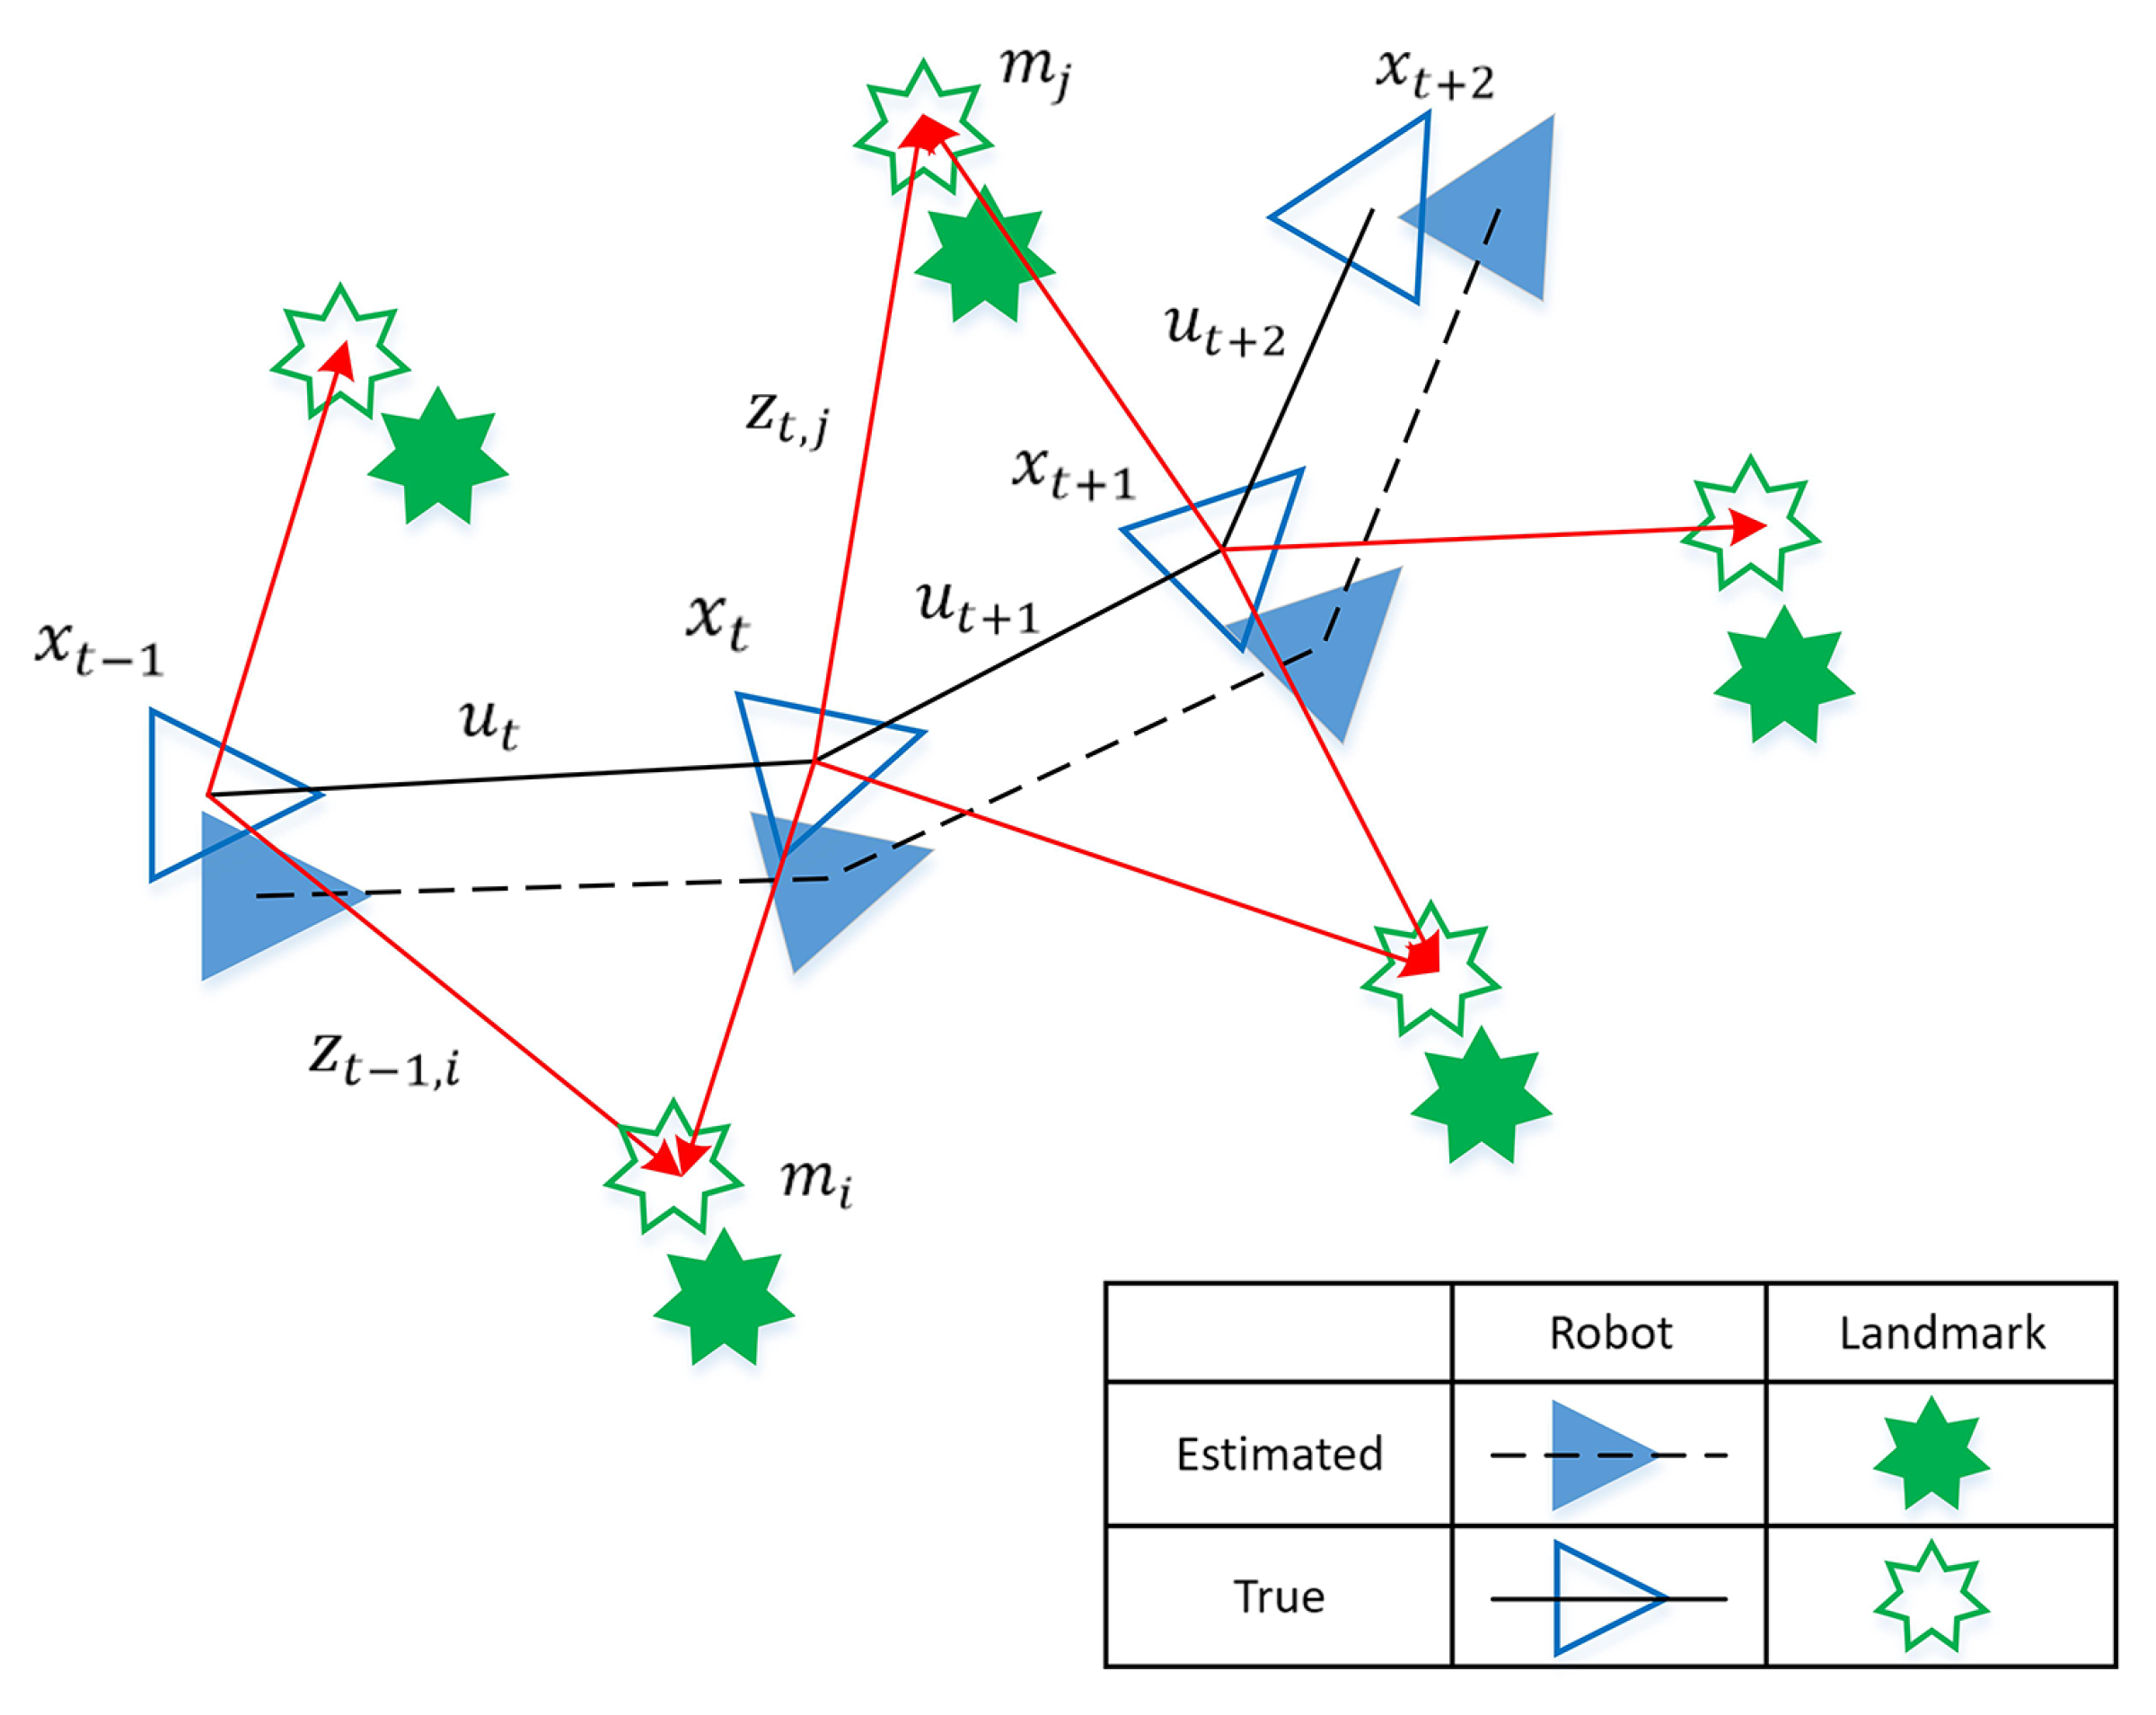
\includegraphics[width=0.4\textwidth]{imgs/SLAM_problrm_modeling.png}
  \caption{SLAM Problem Modeling~\cite{electronics9040695}}
  \label{fig:SLAM-modeling}
\end{figure}

\begin{description}
  \item[Robot state and controls]
        \begin{itemize}
          \item \(\mathbf{x}_t\): the robot's \emph{state vector} at time \(t\), typically \(\bigl[x,y,\theta]\) in ground robots.
          \item \(\mathbf{u}_t\): the \emph{control input} applied between time \(t-1\) and \(t\); by convention \(\mathbf{u}_t\) drives \(\mathbf{x}_{t-1}\to\mathbf{x}_t\).
        \end{itemize}

  \item[Landmarks]
        \begin{itemize}
          \item \(\mathbf{m}_i\): the true position of the \(i-th\) landmark. All landmarks are assumed to be time invariant.
        \end{itemize}

  \item[Observations]
        \begin{itemize}
          \item \(\mathbf{z}_t^i\): the observation of landmark \(i\) taken at time \(t\). When the landmark index is not important, it is written \(\mathbf{z}_t\).
        \end{itemize}

  \item[Histories]
        The full histories of states, controls, and measurements up to time \(t\) are
        \[
          X_{0:t} = \{\mathbf{x}_0,\mathbf{x}_1,\ldots,\mathbf{x}_t\},
          \quad
          U_{0:t} = \{\mathbf{u}_1,\mathbf{u}_2,\ldots,\mathbf{u}_t\},
          \quad
          Z_{0:t} = \{\mathbf{z}_1,\mathbf{z}_2,\ldots,\mathbf{z}_t\}
        \]
        Collect all \(n\) landmarks in the set
        \[
          \mathcal{M} = \{\mathbf{m}_1,\mathbf{m}_2,\dots,\mathbf{m}_n\}
        \]

\end{description}

\subsection{Probabilistic formulation}\label{Probabilisticslam}

In the probabilistic formulation of \gls{slam} the full joint posterior is sought over the robot pose at time $t$ and the map landmarks given all measurements and controls up to $t$:

\begin{equation}
  P\bigl(x_t,\mathcal{M} \mid Z_{0:t},\,U_{0:t},\,x_0\bigr)
  \label{eq:joint-posterior}
\end{equation}

A recursive Bayes filter alternates between prediction (time update) and correction (measurement update) steps:

\paragraph*{Prediction (Time update)}

Assuming a Markovian motion model

\begin{equation}
  P\bigl(x_t\mid x_{t-1},\,u_t\bigr)
  \label{eq:motion-model}
\end{equation}
the prior at time $t$ is
\begin{align}
  P\bigl(x_t,\mathcal{M} \mid Z_{0:t-1},\,U_{0:t},\,x_0\bigr)
   & = \int
  P\bigl(x_t\mid x_{t-1},\,u_t\bigr)\,
  P\bigl(x_{t-1},\mathcal{M} \mid Z_{0:t-1},\,U_{0:t-1},\,x_0\bigr)
  \,\mathrm{d}x_{t-1}
  \label{eq:time-update}
\end{align}

\paragraph*{Correction (Measurement update)}
With the observation model

\begin{equation}
  P\bigl(z_t\mid x_t,\mathcal{M}\bigr)
  \label{eq:obs-model}
\end{equation}

the new measurement $z_t$ is incorporated through

\begin{align}
  P\bigl(x_t,\mathcal{M} \mid Z_{0:t},\,U_{0:t},\,x_0\bigr)
   & = \frac{P\bigl(z_t\mid x_t,\mathcal{M}\bigr)\,
    P\bigl(x_t,\mathcal{M} \mid Z_{0:t-1},\,U_{0:t},\,x_0\bigr)}
  {P\bigl(z_t\mid Z_{0:t-1},\,U_{0:t}\bigr)}
  \label{eq:meas-update}
\end{align}

where the denominator is the normalizing constant~\cite{1638022}.

\subsection{RTAB-Map}\label{subsec:rtabmap}

\gls{rtab} is a graph-based visual \gls{slam} system that leverages loop-closure reasoning.
In \gls{rtab}, image feature extraction is the first step in enabling appearance based localization and loop-closure detection. This process involves transforming a raw sensor image $I_t$ into a descriptive image signature $s_t$ that can be efficiently compared against past images.

\begin{figure}[H]
  \centering
  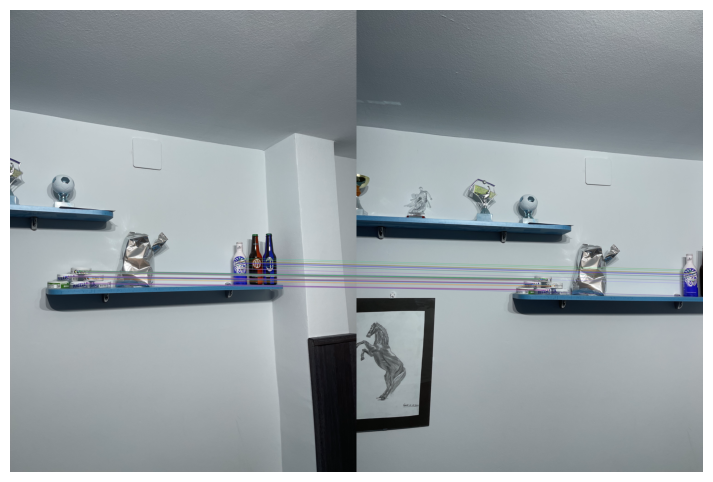
\includegraphics[width=0.5\linewidth]{imgs/image_feature_extraction.png}
  \caption{Feature matching of an image}
  \label{fig:feature_extraction}
\end{figure}

\MakeUppercase{t}hese signatures are constructed in a pipeline of 3 steps (see~\cite{1570189} for more details):

\begin{enumerate}
  \item Saliency Detection
  \item Wide-Baseline Stability
  \item Descriptor Computation
\end{enumerate}

\MakeUppercase{t}hese signatures are mapped into a vector using the \gls{bovw} approach to reduce the high dimensionality, also \gls{tfidf} weighting is adopted to give less importance to low information signatures.

\begin{equation}
  \mathbf{s}_{t,I}=tf_{t,I}\;\log\frac{N}{df_t} \label{eq:tfidf}
\end{equation}

where $N$ is the total number of locations created so far, $df_t$ the locations containing $s_t$ and $tf_{t,I}$ the frequency of $t$ in $I$.

\subsubsection*{Loop-closure detection}

Once a new \gls{tfidf} signature $\mathbf{s}_t$ has been built, \gls{rtab}
searches for a previously created location that visually matches the current
view while respecting real-time constraints~\cite{6459608}.

\begin{enumerate}[label=\alph*)]
  \item \textbf{Similarity scoring}
        For each candidate location $i$ stored in \gls{wm}, a similarity defined as

        \begin{equation}
          S(s_t, s_c) =
          \begin{cases}
            N_{\text{pair}} / N_{s_t}, & \text{if } N_{s_t} \geq N_{s_c} \\
            N_{\text{pair}} / N_{s_c}, & \text{if } N_{s_t} < N_{s_c}
          \end{cases}
        \end{equation}

        measures appearance overlap, where $N_{pair}$ is the number of matched word pairs between
        the compared location signatures, and where $N_{s_t}$ and $N_{s_c}$ are
        the total number of words of signature $s_t$ and the compared
        signature $s_c$ respectively.

  \item \textbf{Bayesian evidence accumulation}
        Denoted by $\mathcal{H}_t$ the hypothesis that the robot is revisiting location $i$.
        Similarities feed a discrete Bayesian filter that updates $P(\mathcal{H}_t)$.


        \begin{equation}
          p(\mathcal{H}_t\!\, \mid L^t) = \eta~\underbrace{p(L_t \mid \mathcal{H}_t\!\,)}_{\text{Observation}}
          \underbrace{\sum_{i=-1}^{t_n}
            \underbrace{p(\mathcal{H}_t\!\, \mid \mathcal{H}_{t-1}\!\, = i)}_{\text{Transition}}
            p(\mathcal{H}_{t-1}\!\, = i \mid L^{t-1})}_{\text{Belief}}
        \end{equation}

        where $L_t$ is a location created with signature $s_t$, $L^t=L_1,\dots,L_t$ and $\eta$ is a normalizing term.

  \item \textbf{Decision rule}
        A loop-closure is declared when the most probable hypothesis exceeds a fixed
        threshold:

        \begin{equation}
          \max_i P(\mathcal{H}_t \mid L^t) \;\ge\; T_{\mathrm{LC}}.
          \label{eq:lc-threshold}
        \end{equation}

        The nodes $L_t$ and $L_i$ are then linked to the pose graph, and any spatial neighbors of $L_i$ that reside in \gls{ltm} are retrieved back into \gls{wm} to improve future detections.

  \item \textbf{Memory management.}
        When the per-frame processing time $t_{\text{proc}}$ exceeds a user defined limit $T_{\text{time}}$, the transfer step removes the oldest of the
        least viewed locations (smallest weight $w_i$) from \gls{wm} to \gls{ltm}, ensuring
        that real-time performance is maintained.
\end{enumerate}

\section{Mecanum wheels}\label{mecanum}

\begin{figure}[H]
  \centering
  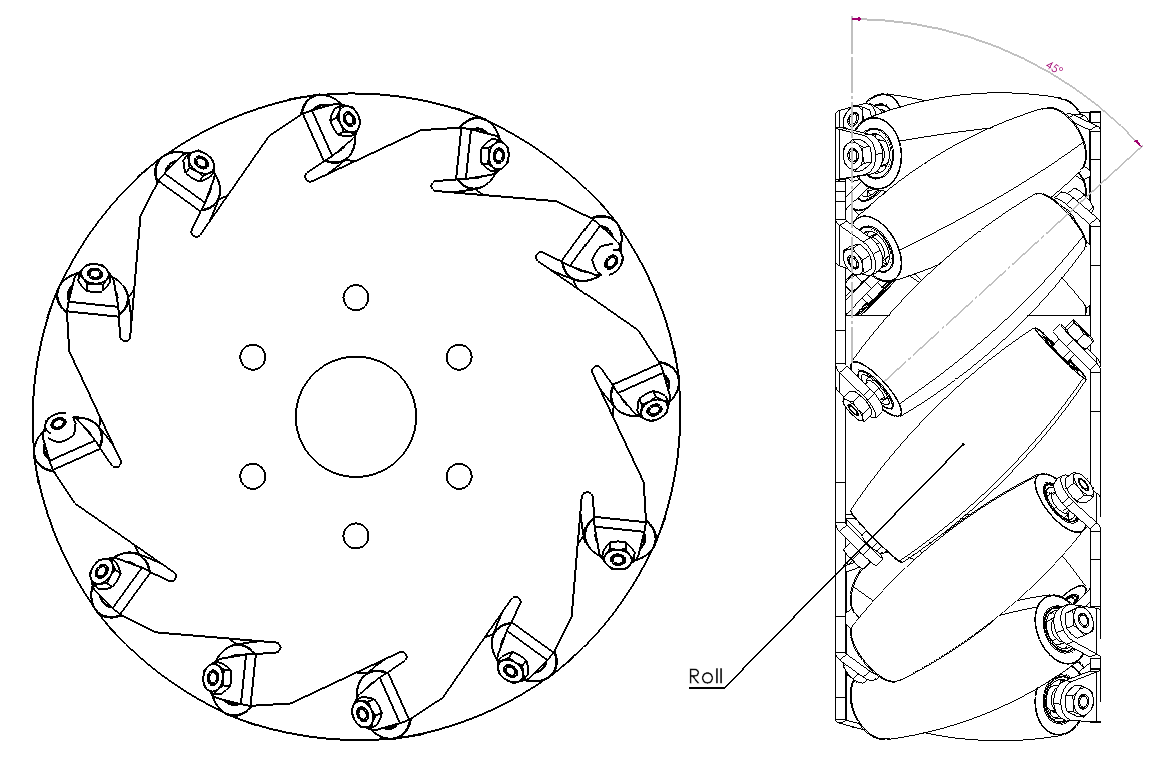
\includegraphics[width=0.5\linewidth]{imgs/mecanum_wheel.png}
  \caption{Mecanum wheel}
  \label{fig:mecanum_wheel}
\end{figure}

Mecanum wheels have been invented to overcome the limitation of maneuverability in robots, especially when navigating complex or tight terrains, their mechanism centers on a uniquely structured wheel designed to facilitate omnidirectional motion while maintaining a high degree of course stability. Each wheel is composed of a central rotating component and a series of ground contacting elements referred to as rolls distributed around its periphery as shown in Figure~\ref{fig:mecanum_wheel}. The key design features include~\cite{US3876255A}:

\begin{enumerate}[label=\textbullet]
  \item \textbf{Roll Configuration:}
        Each ground engaging element is shaped as an elongated roll with a convex surface along its longitudinal axis. These rolls are mounted obliquely to the primary rotational axis of the wheel, usually at an angle between $30\degree$ and $60\degree$.
  \item \textbf{Unbroken Periphery:}
        The geometric arrangement of the rolls ensures a continuous outer wheel surface that allows only one roll to be in contact with the ground at any given moment during standard motion. This structural feature eliminates gaps that could otherwise cause bumping or uneven motion during operation and improves traction, particularly on hard surfaces where multiple point contact could reduce grip.
\end{enumerate}

\begin{figure}[H]
  \centering
  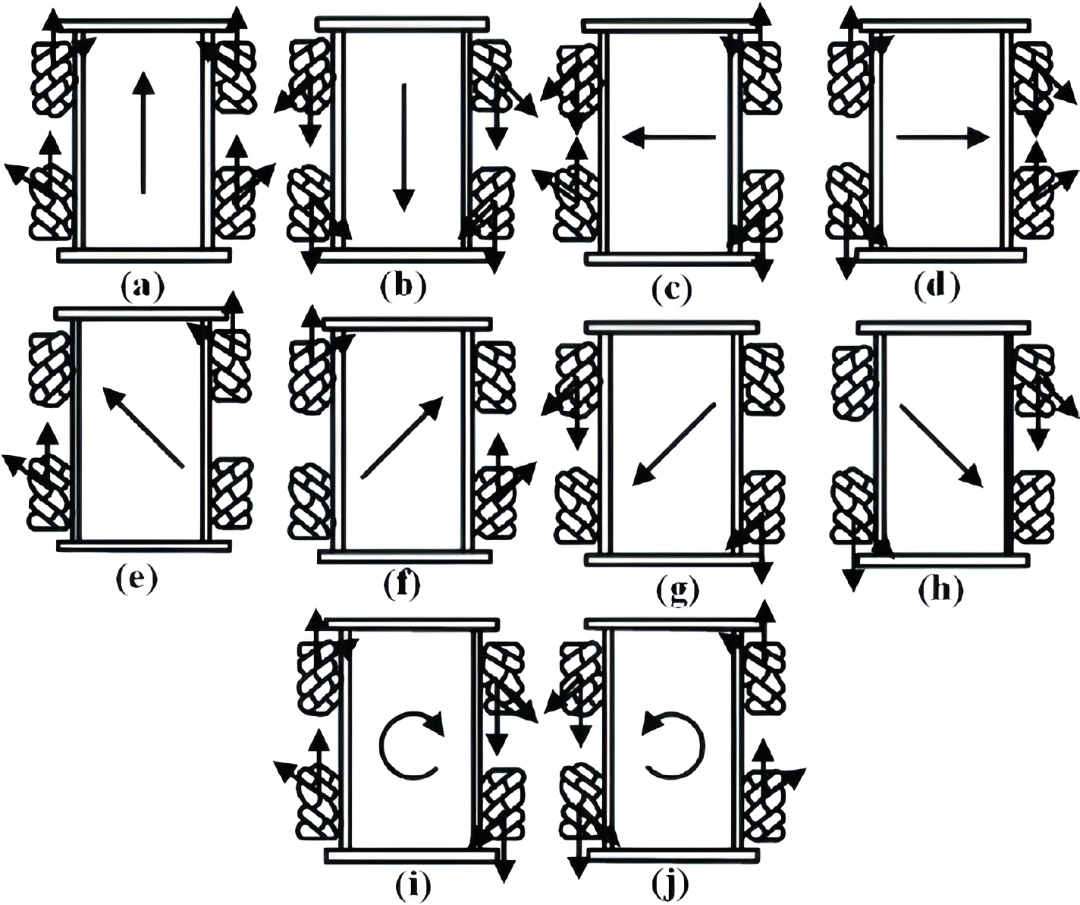
\includegraphics[width=0.3\textwidth]{imgs/mecanum_directions.png}
  \caption{Top view of turning principle of Mecanum wheel~\cite{Shao}}
  \label{fig:mecanum_direction}
\end{figure}

The arrangement depicted in Figure~\ref{fig:mecanum_direction} where each wheel is controlled by a separate motor shows how by varying the direction of rotation and relative speeds of the four wheels, the robot can be moved along any trajectory in the plane and, even more impressively, can simultaneously spin around its vertical axis~\cite{Siegwart2011}.

\section{LiDAR}\label{lidar}

\gls{lidar} is a type of sensor that applies the method of sending laser light on a target and analyzes the light reflected to process its arrival time, it generates a precise mapping of the environment that it scans, and it usually covers $360\degree$ in 2D or 3D where the data it returns is commonly called \emph{pointcloud}~\cite{mehendale2020review}.

\begin{figure}[H]
  \centering
  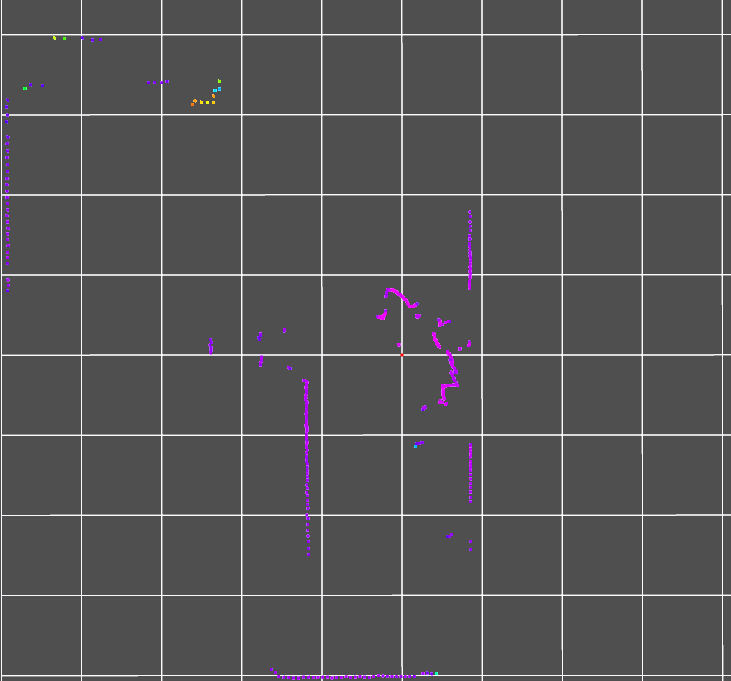
\includegraphics[width=0.3\textwidth]{imgs/pointcloud.png}
  \caption{2D pointcloud generated by a LiDAR sensor}
  \label{fig:pointcloud}
\end{figure}

\subsection{Working principle}

The main idea behind \gls{lidar} is the reflection of light, the \gls{lidar} sends a laser beam to the target and measures the time variation of the reflect light, from these calculations, it calculates the distance to draw the pointcloud of the target. The formula for calculating the distance is

\begin{equation}
  D = \frac{c \cdot \Delta T}{2}
  \label{eq:1}
\end{equation}

\section{Stereo vision}

Stereo vision recovers the 3D structure of a scene by combining two images acquired from different viewpoints. In its simplest form, two cameras are placed with their optical axes parallel and separated by a baseline \(T\). A point \(P=(X,Y,Z)\) in space projects to image coordinates \((x_\ell,y_\ell)\) and \((x_r,y_r)\) in the left and right cameras (Figure~\ref{fig:stereo-rig}), respectively, via

\[
  (x,y) = \bigl(f\,X/Z,\;f\,Y/Z\bigr),
\]

where \(f\) is the focal length.

\begin{figure}[H]
  \centering
  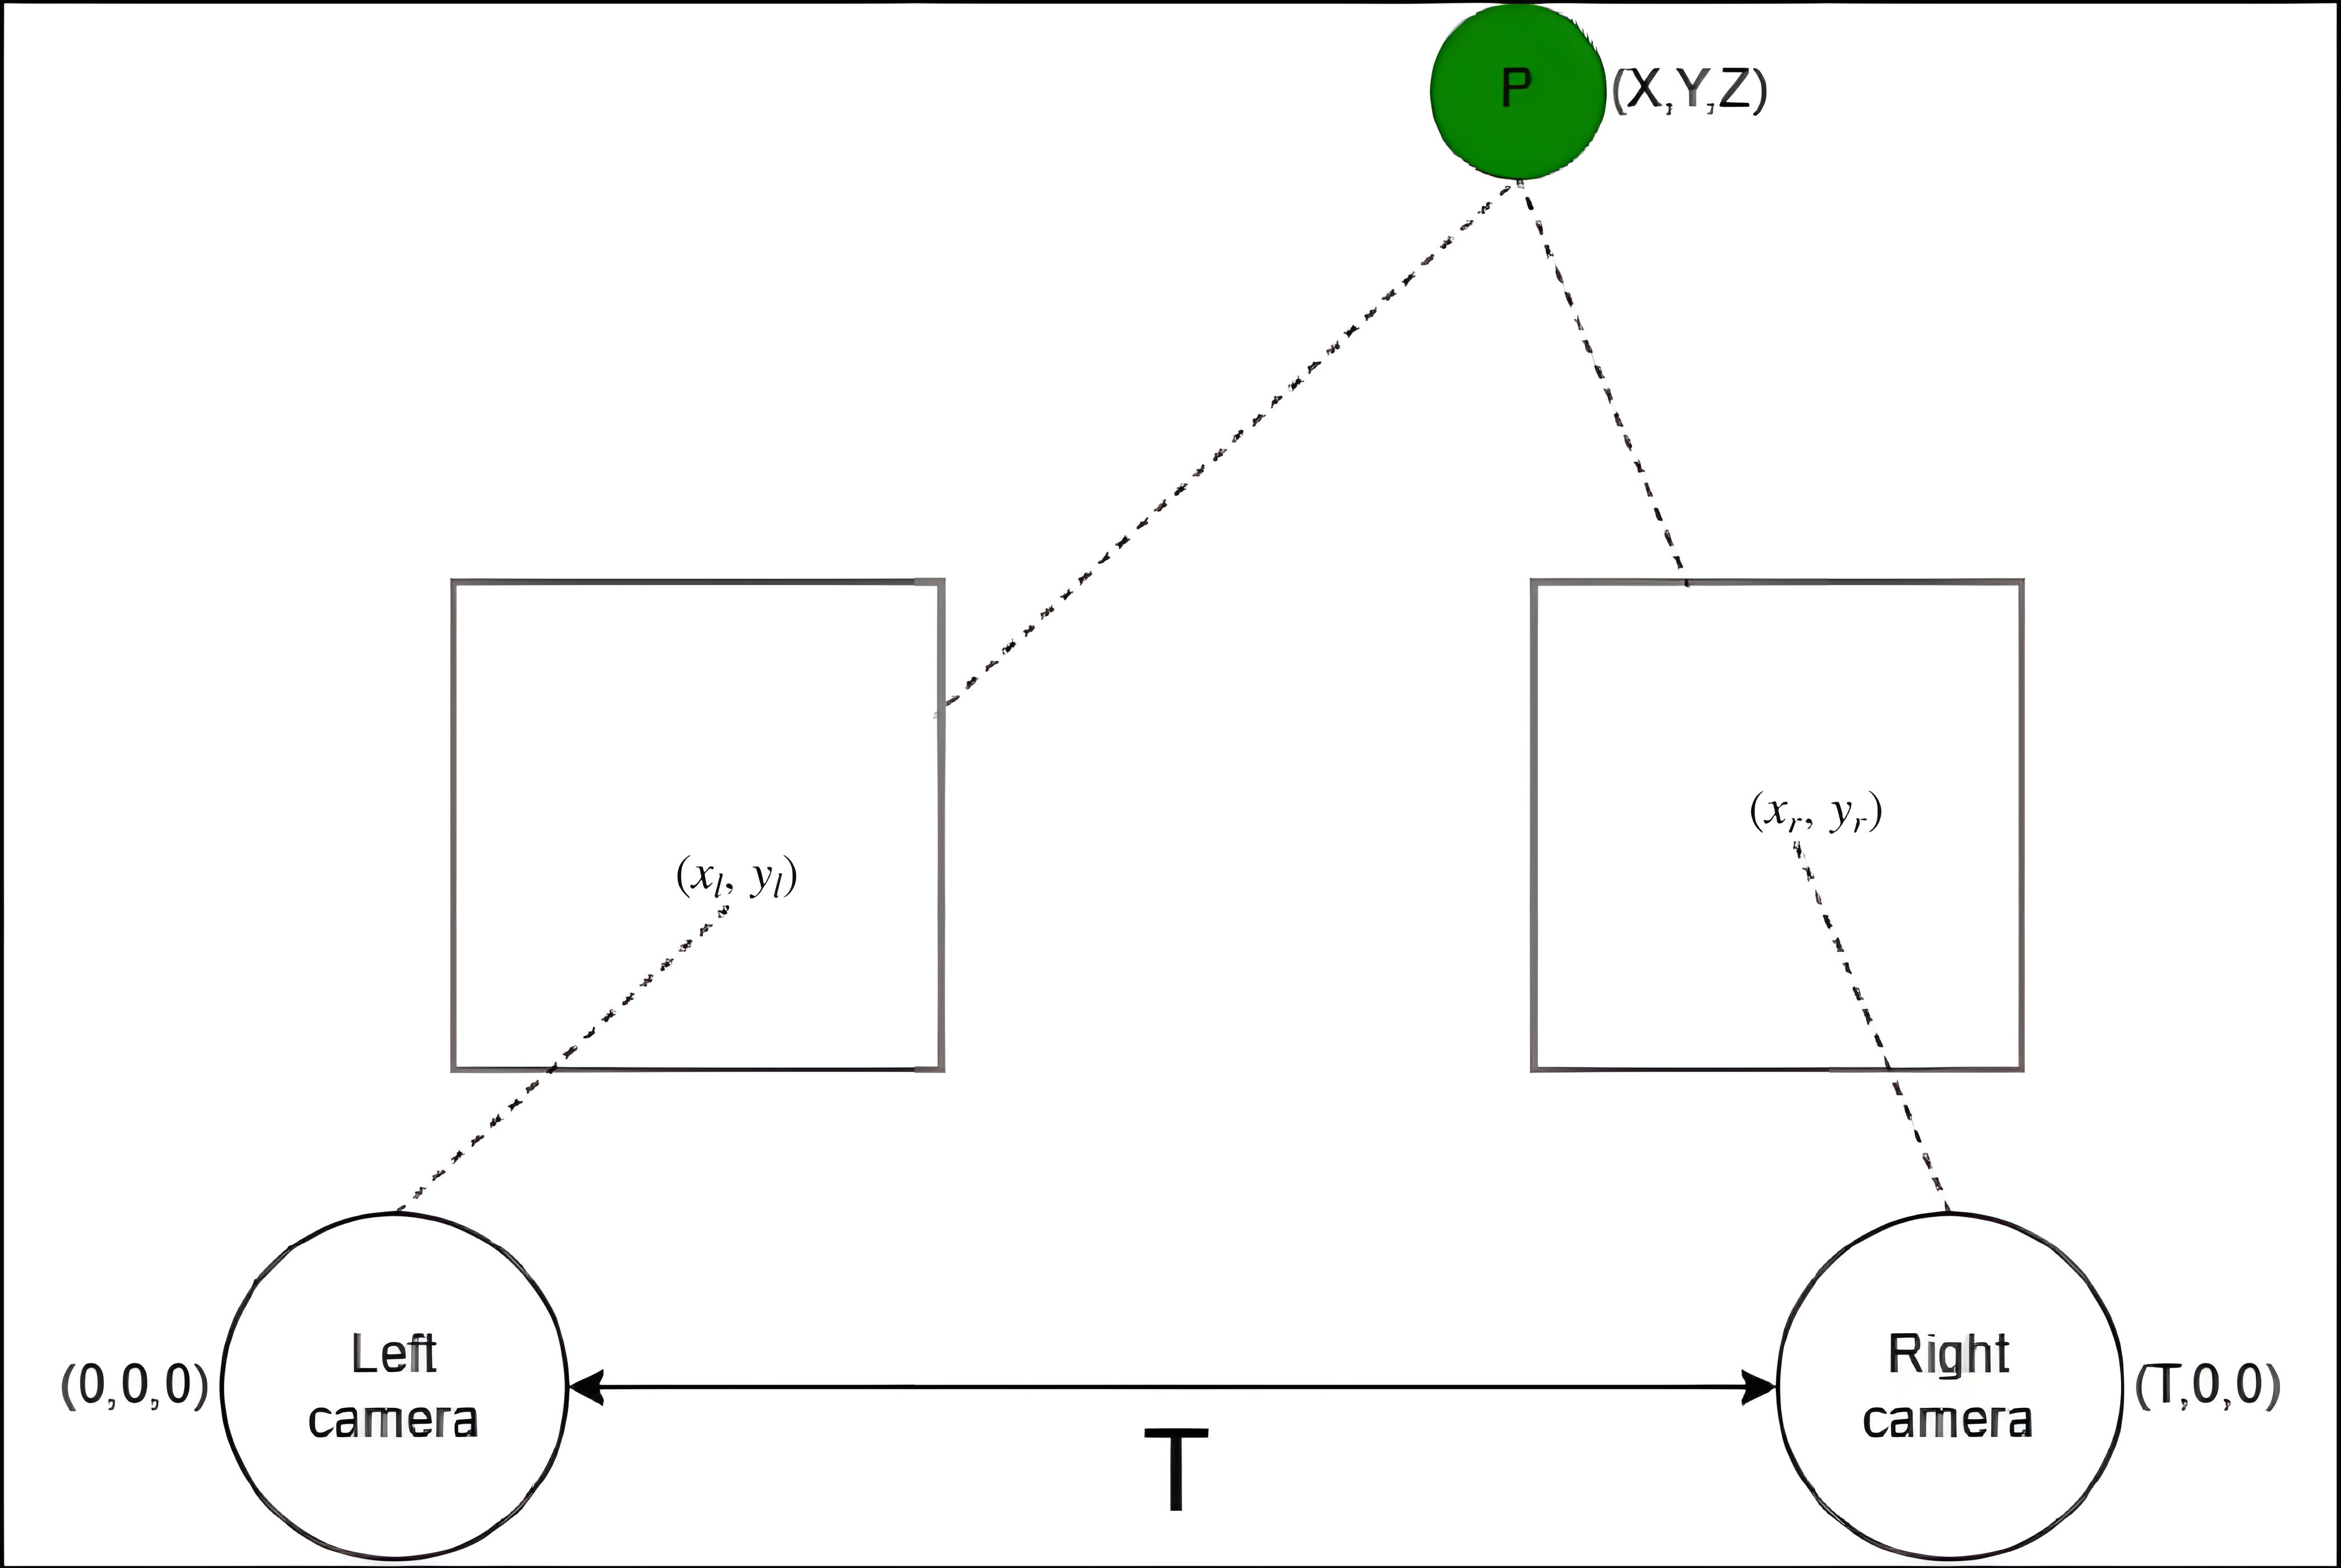
\includegraphics[width=0.6\textwidth]{imgs/rig.png}
  \caption{Side view of a stereo rig: two cameras separated by baseline \(T\), parallel optical axes, and back-projection rays through \(P\)}
  \label{fig:stereo-rig}
\end{figure}

By definition of the rectified configuration, \(y_\ell = y_r\) and the \emph{disparity} \(d = x_\ell - x_r\) encodes depth:
\[
  Z = \frac{f\,T}{d}
\]
Thus nearby points produce large disparities, and distant points small ones.

\begin{figure}[H]
  \centering
  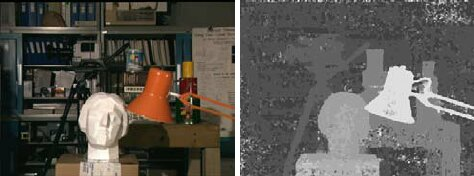
\includegraphics[width=0.6\textwidth]{imgs/A-reference-image-and-its-estimated-disparity-map-The-disparity-map-appears-noisy-since_W640.jpg}
  \caption{Disparity map~\cite{inproceedings}}
  \label{fig:disparity-map}
\end{figure}

A basic computational pipeline for stereo vision is:
\begin{enumerate}
  \item \textbf{Feature Matching:} for each pixel in the left image, search along its scan line in the right image to find the best match.
  \item \textbf{Disparity Refinement:} enforce smoothness priors and left/right consistency to eliminate outliers.
  \item \textbf{Depth Computation:} convert each refined disparity \(d\) to depth \(Z = \frac{f\,T}{d}\).
\end{enumerate}

\section{CAN bus}\label{can}

\gls{can} is a serial, multi \gls{masterslave}, differential communication protocol designed for distributed control in real-time, critical to safety. It enables devices to exchange short messages over a single shared bus.

\begin{figure}[H]
  \centering
  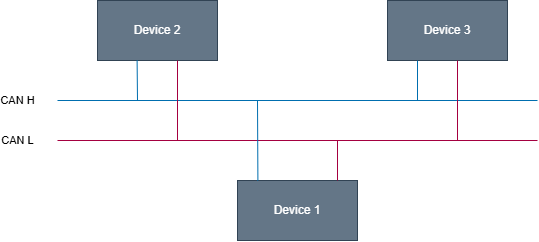
\includegraphics[width=0.5\textwidth]{imgs/canbus.png}
  \caption{Devices in a CAN bus}
  \label{fig:cannet}
\end{figure}

\subsection{Wiring}

Two communication wires are utilized to transmit data simultaneously, referred to as CANH (High) and CANL (Low), each operating at distinct voltage levels recognized by the devices. Typically, CANH operates within a range of \SI{2.5}{\volt} to \SI{3.75}{\volt}, while CANL ranges from \SI{2.5}{\volt} to \SI{1.25}{\volt}. When both wires show a voltage of \SI{2.5}{\volt}, it corresponds to a binary value of 1. Conversely, when CANH reaches \SI{3.75}{\volt} and CANL drops to \SI{1.25}{\volt}, the signal represents a binary value of 0. the protocol prioritizes the detection of 0 values rather than 1 values. Therefore, the driver logic operates inversely compared to standard digital logic interpretation~\cite{bosch1991can}.

\subsection{Message structure \& format}
Every \gls{can} DATA frame consists of

\begin{itemize}
  \item \textbf{Start of Frame:} A single dominant bit marking the start of the frame.
  \item \textbf{Arbitration Field:}
        \begin{itemize}
          \item 11-bit (standard) or 29-bit (extended) identifier.
          \item Remote Transmission Request bit: Indicates whether data is being sent or requested.
        \end{itemize}
  \item \textbf{Control Field:}
        \begin{itemize}
          \item 4-bit Data Length Code: Specifies the number of data bytes (0-8).
          \item Includes 2 reserved bits.
        \end{itemize}
  \item \textbf{Data Field:} Contains 0 to 8 bytes of data.
  \item \textbf{CRC Field:}
        \begin{itemize}
          \item 15-bit Cyclic Redundancy Check sequence for error detection.
          \item 1-bit CRC delimiter (logical 1).
        \end{itemize}
  \item \textbf{ACK Field:}
        \begin{itemize}
          \item ACK Slot: to indicate if an error is detected.
          \item ACK Delimiter (logical 1) so the ACK slot is surrounded by two logical 1 bits.
        \end{itemize}
  \item \textbf{End of Frame:} Seven bits.
\end{itemize}

\begin{figure}[H]
  \centering
  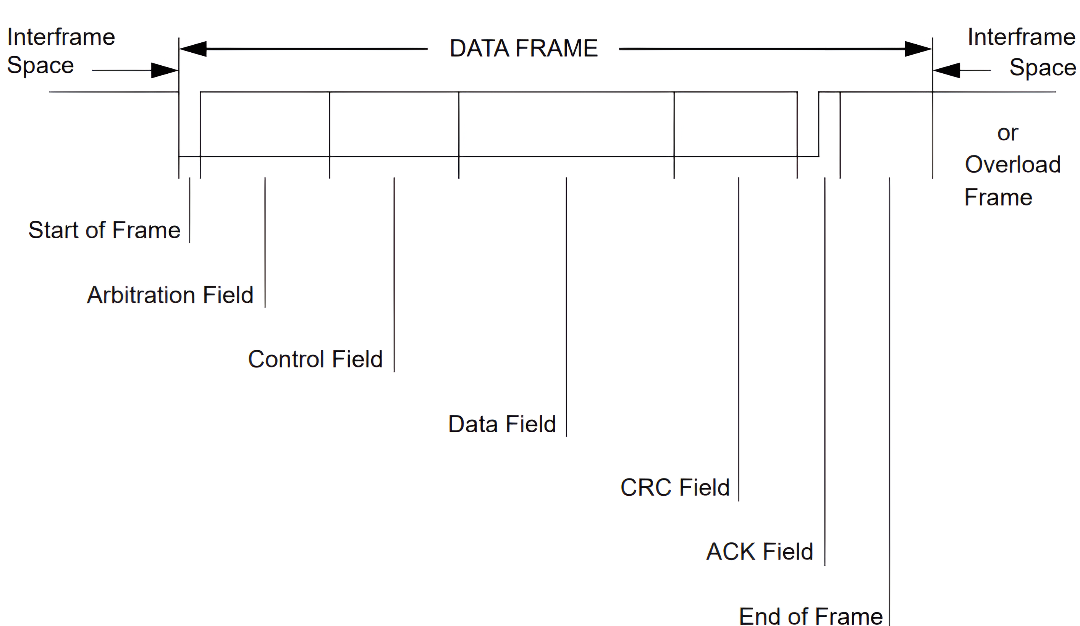
\includegraphics[width=0.7\textwidth]{imgs/can_data_structure.png}
  \caption{CAN data structure~\cite{bosch1991can}}
  \label{fig:candata}
\end{figure}

\section{ROS 2}

\gls{ros} is an open-source middleware that increases the system's capabilities to develop robotics applications, it provides tools and libraries that make it easier to merge sensors and control them.

At runtime, a \gls{ros}~2 system is described by its computation graph. Nodes advertise their functionality by publishing or subscribing to topics, invoking or serving services, or sending and receiving actions. Topics support many-to-many, asynchronous data streams (for example, camera images or laser scans), whereas services and actions enable request/response and long running goal semantics, respectively. Figure~\ref{fig:comp-graph} shows a minimal example in which a camera driver node publishes raw images, a perception node subscribes to those images to detect obstacles, and a control node issues velocity commands to the robot base.

\begin{figure}[H]
  \centering
  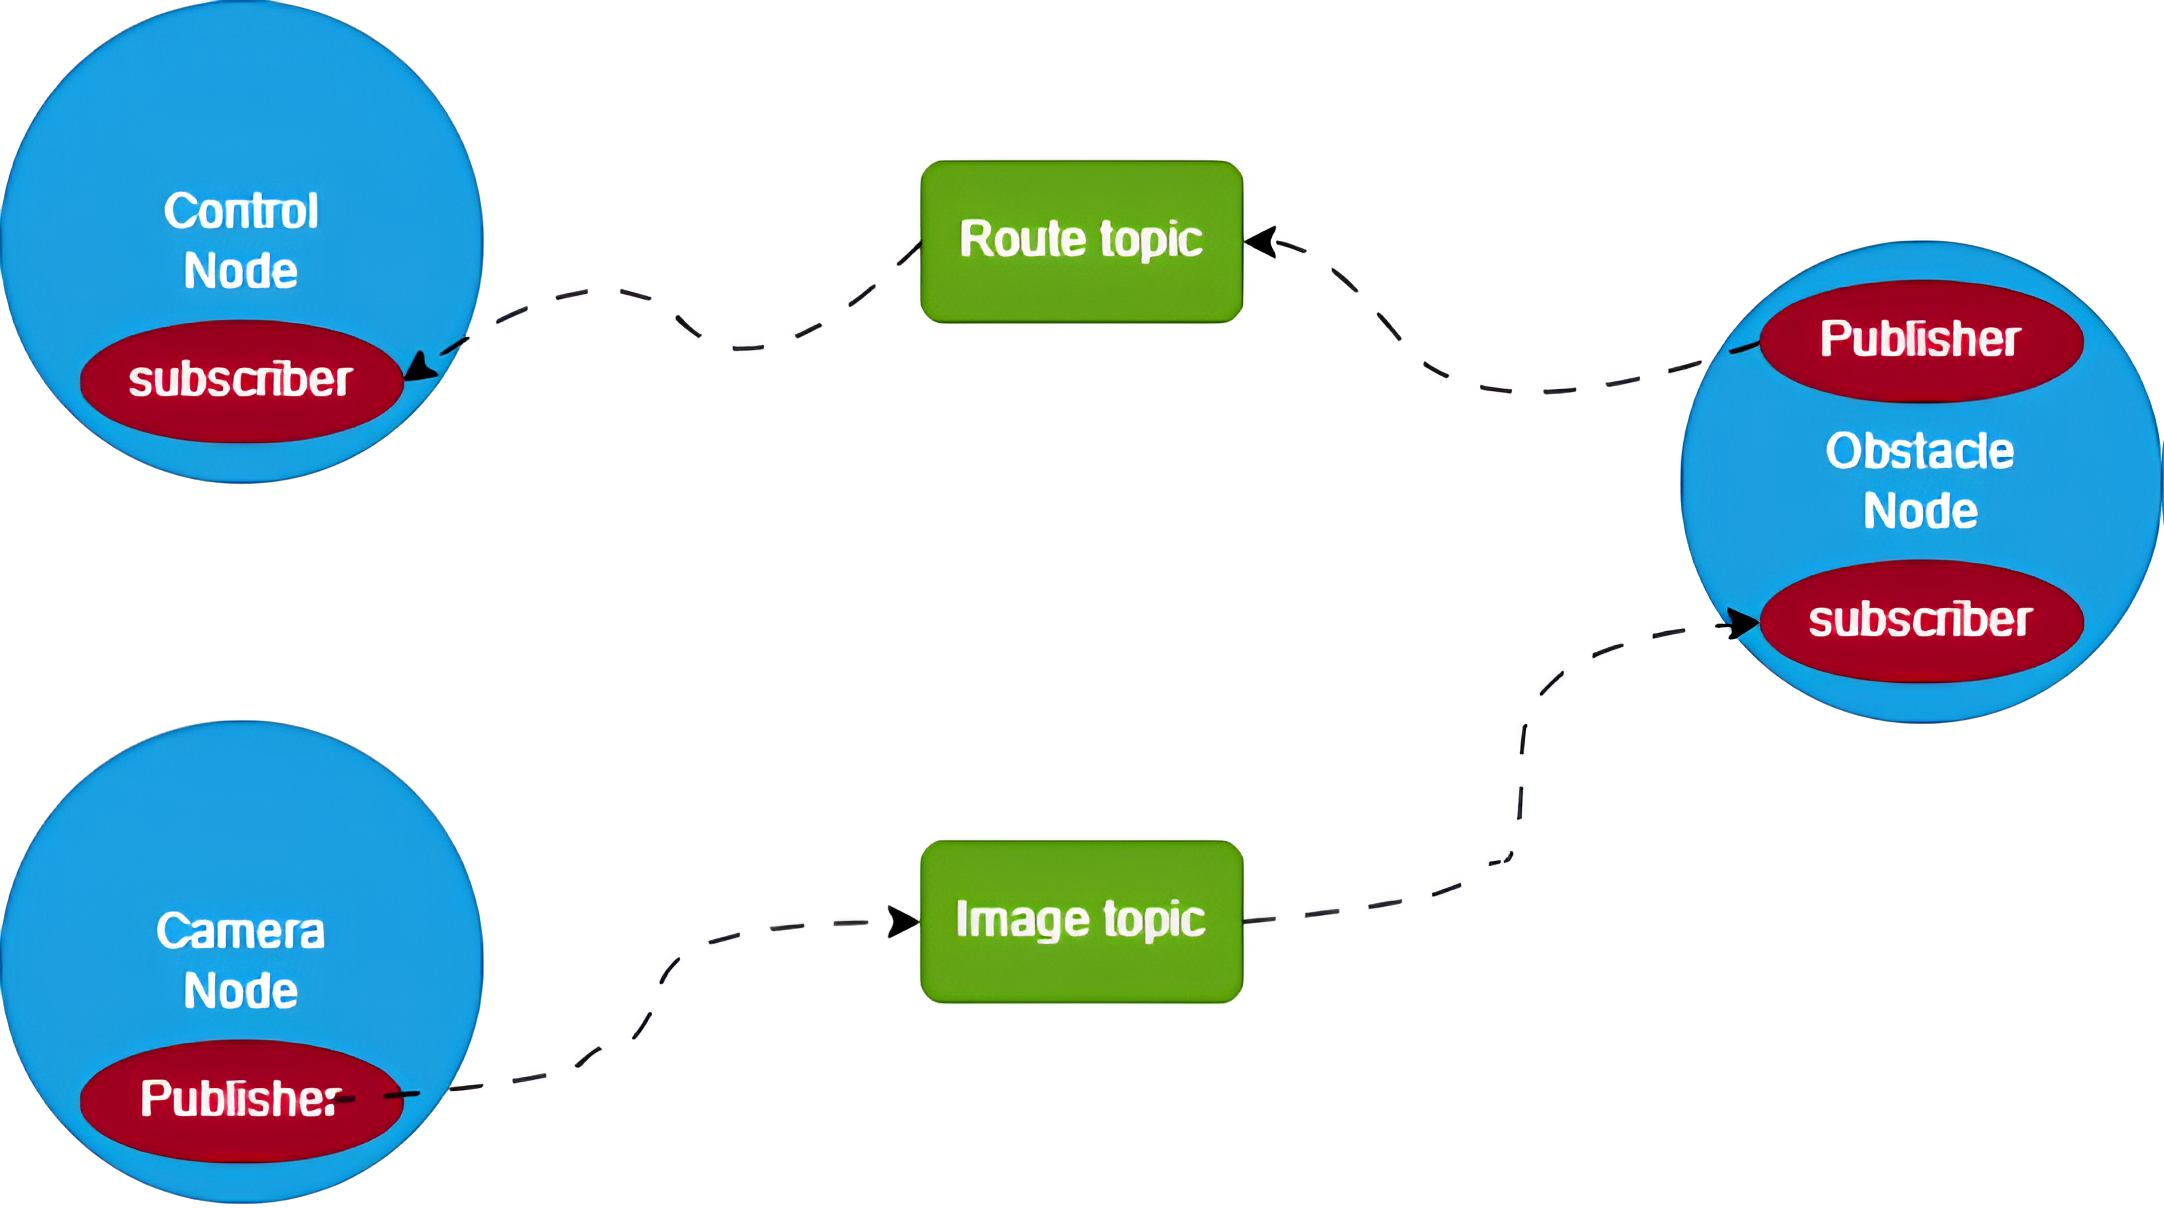
\includegraphics[width=0.8\textwidth]{imgs/ros.png}
  \caption{ROS 2 computation graph}
  \label{fig:comp-graph}
\end{figure}

Developers organize their sources into a \texttt{colcon} workspace. Within this workspace, each \gls{ros}~2 package declares its own build and runtime dependencies, message and service definitions, and executable entry points. A single invocation of \texttt{colcon build} starts compilation, interface generation and installation, resulting in a unified directory structure from which nodes may be launched.

\chapter{System architecture}\label{chap:system_architecture}

This chapter presents a high-level view of the robot. It describes the logical organization of subsystems, the flow of information and power, and the design considerations that drive each interface. By focusing on conceptual elements rather than specific parts, this chapter lays the groundwork for later detailed component selections and implementation.

\section{Mobility overview}

A primary design decision concerns locomotion. The robot is intended to navigate in indoors environments, which suggests tight space implying the use of omnidirectional drive systems.
Here is a comparison of some that were taken into consideration~\cite{Siegwart2011}

\begin{itemize}
  \item \textbf{Spherical wheels}:Based on spherical wheels (usually three), each actuated by a separate motor, The spherical wheels are supported by three contact points: two are achieved through spherical bearings, while the third is provided by a wheel attached to the motor axle. This design offers ease of maneuverability and a straightforward structure. Nevertheless, it is confined to level surfaces and light loads.
  \item \textbf{Mecanum (see chapter~\ref{mecanum}) wheels}
  \item \textbf{Swerve Drive Systems}:Swerve drives are among the best omnidirectional systems. Each wheel is independently mounted on a rotating module that can turn to face any direction, while also being driven to control speed. The downside of this system is the high complexity, being that each wheel is controlled by a motor and a \gls{servo} for the rotation.
\end{itemize}

As the robot is intended to function autonomously with significant weight that discards the first option. The third option implies eight actuators which elevates the complexity of the system a significant amount, therefore, Mecanum wheels were selected as they provide all the necessary mobility with the ease of use.

\section{Conceptual overview}\label{sec:conceptual_overview}

Controlling the four motors precisely, pose estimation, power supply and processing the algorithms is still pending, taking into account two important concepts

\begin{enumerate}
  \item Components' safety:
        Incorporate mechanisms for preventing and detecting failures.
  \item Modularity and Scalability:
        Allow future upgrades such as additional sensors and actuators.
\end{enumerate}

The first step is managing the four motors, speed and direction control is needed, for that an \gls{hbridge} driver can be used, which allows both controls to with logical and \gls{pwm} inputs. The generation of these signals is handled by a \gls{mcu} allowing for real-time data acquisition of the speed for analysis and adaptive signal control for motor response.

An \gls{mcu} by its nature has small computational power for running complicated algorithms, specially when involving image analysis and computer vision, so a second high level processor must be used, on top of that, the integration of hardware needed for the \gls{slam} execution is almost impossible in a normal \gls{mcu}. On top of that, it is always a good practice to separate motor control form main components mainly for the reverse voltage and signal noise that it generates due its nature of having a magnetic field.

Having two controllers, a communication protocol is necessary between them, as scalability is a main concern, \gls{can} has been chosen (see chapter~\ref{can}) being a multi \glspl{masterslave} protocol, also, it will not be affected by the noise generated by the motors being differential.

As for the \gls{slam} hardware, two components are essential, the \gls{lidar} and an \gls{rgbd} camera, allowing for the visual and spatial construction of the scene.

With these principles set, the only thing left is the power supply to run all these components safely, for that a battery with a \gls{bms} is highly recommended, avoiding the damage that can be caused due to the reverse voltage of the motors and supplying enough power to all components rather than depending on one of the processors that break due to the consumption.

\chapter{Component selection}\label{chap:component_selection}

The component selection process for the robot was guided by a clear methodology, defining technical and practical criteria that the component must comply, and assuring that the component can be integrated into the system smoothly.
To begin, narrative criteria is established. Electrically, every part had not to exceed a nominal voltage of \SI{22.2}{\volt}, which is the voltage supplied by the battery that will be integrated into the system. From a physical standpoint, the components must fit in the chassis design (as shown in chapter~\ref{design}). Finally, the \gls{mcu} must have all the required pins and timers to perform the data acquisition and signal generation, and the motor must generate enough torque speed for the weight of the robot.\\
Figure~\ref{fig:block-diagram} presents a high-level view of the robot's architecture. The 6 S LiPo battery and \gls{bms} supply three regulated rails (\SI{3.3}{\volt} for the \gls{mcu} and low-power sensors, \SI{5}{\volt} for logic and driver modules, and \SI{12}{\volt} for the \textbf{Jetson Orin Nano}). The \textbf{Jetson} and \textbf{STM32F303RE} exchange speed setpoints and encoder feedback over \gls{can} bus; the \textbf{STM32} captures \gls{hall} signals, generates \gls{gpio}/\gls{pwm} control for the dual \gls{hbridge} drivers, and drives the four geared DC motors. Sensors feed perception data into the \textbf{Jetson}, and a local display visualizes live status and maps.

\begin{figure}[H]
  \centering
  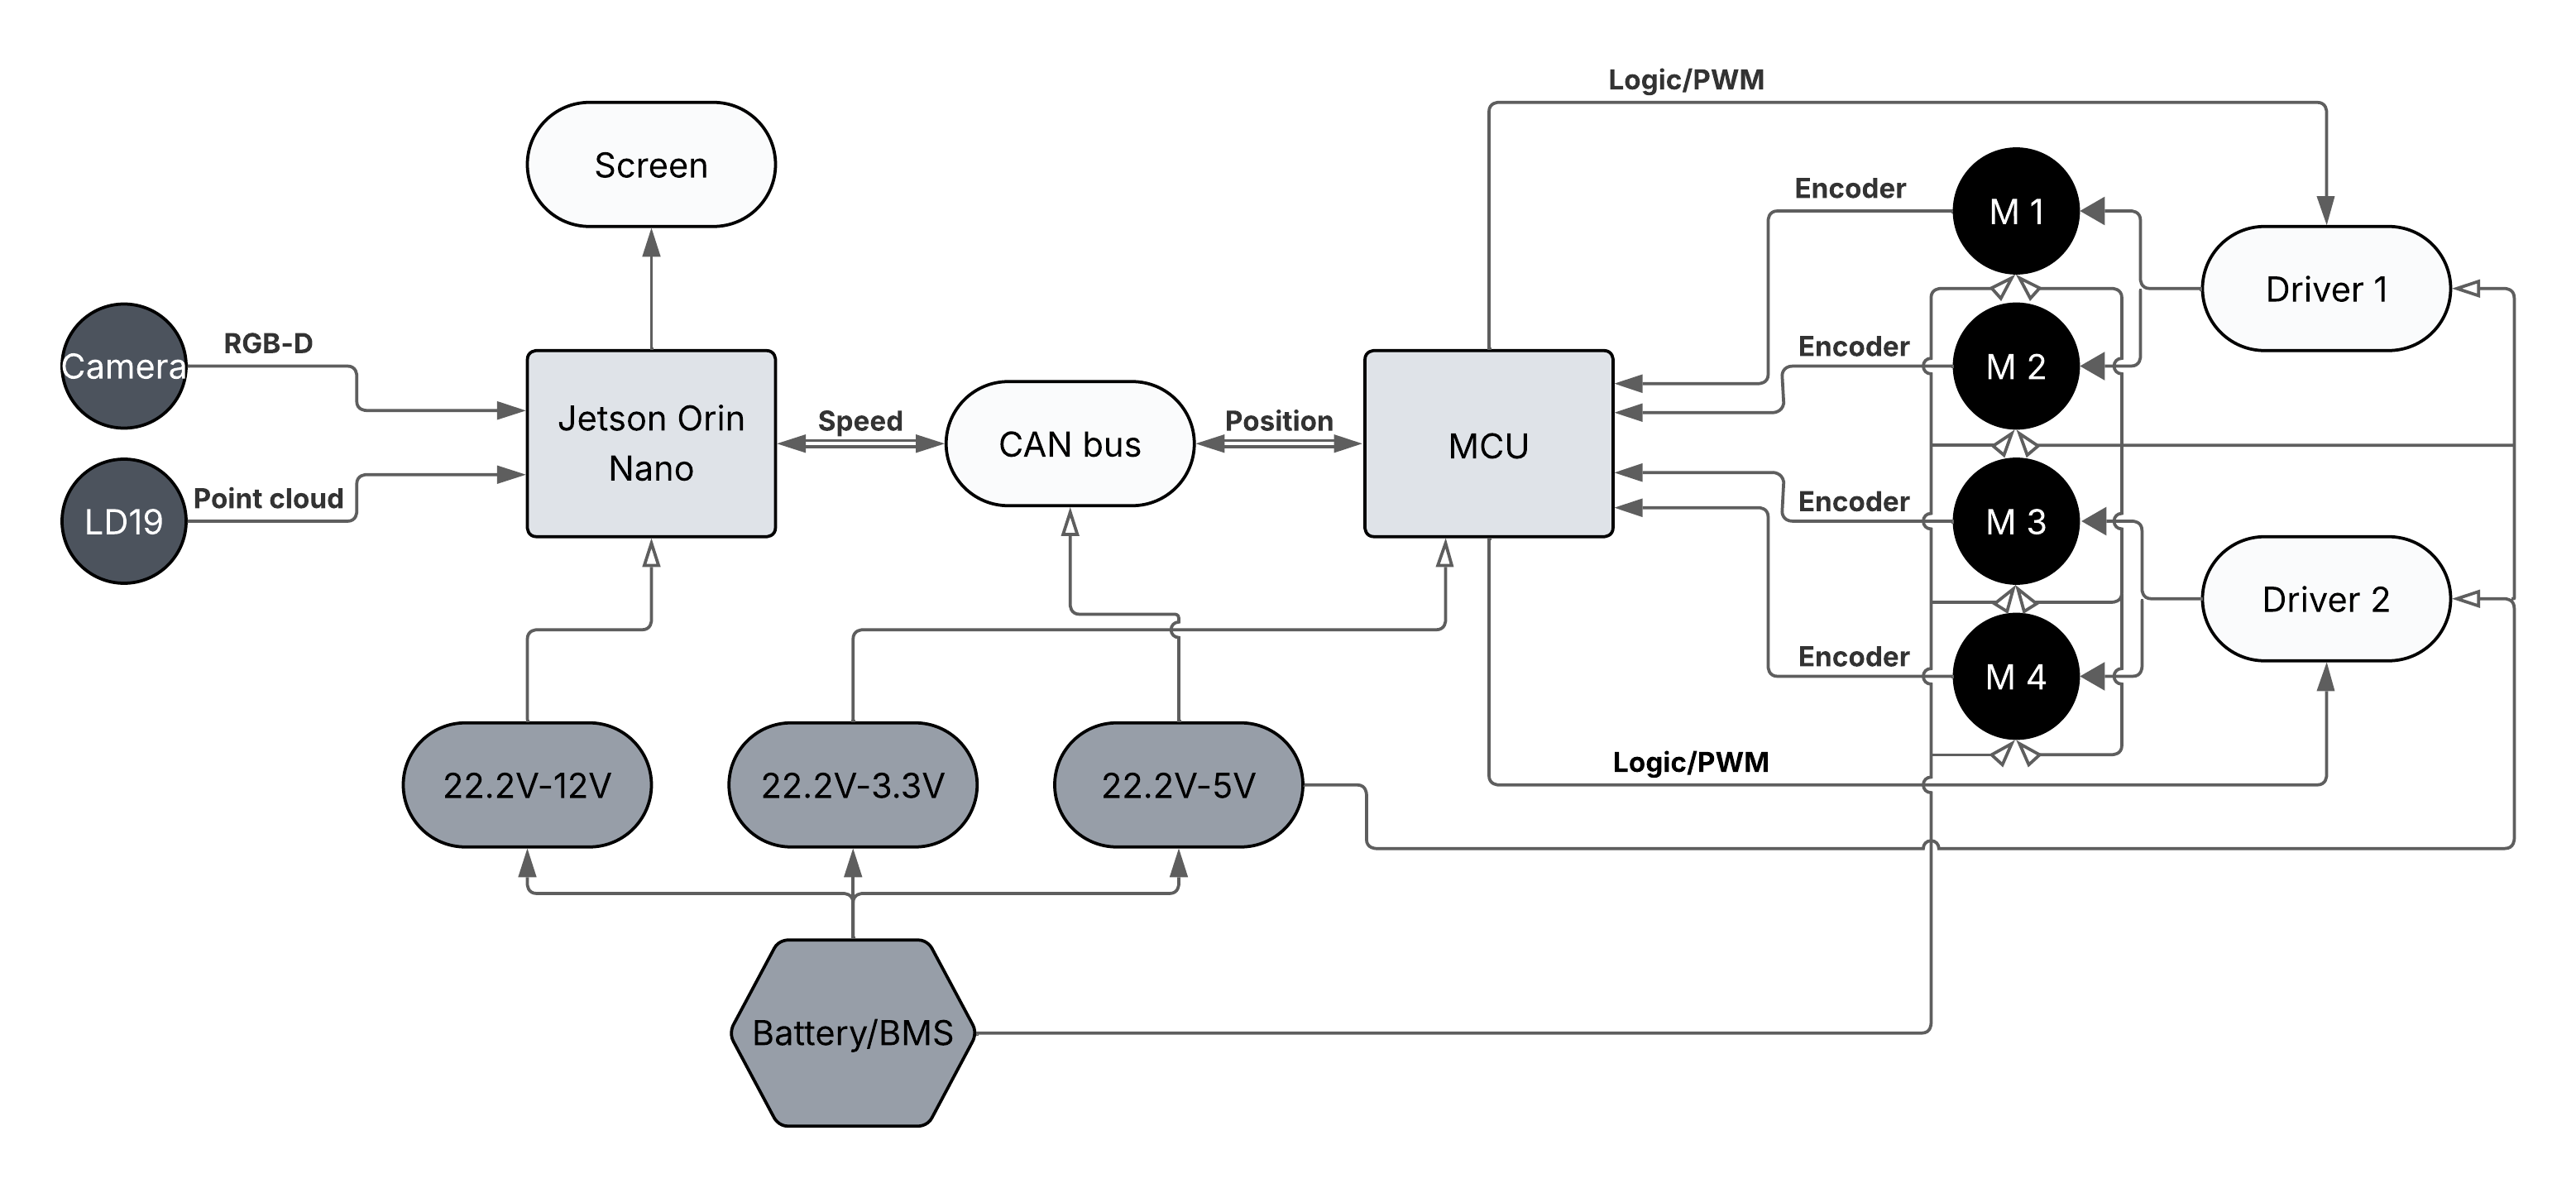
\includegraphics[width=0.8\textwidth]{imgs/blockdiagram.png}
  \caption{System block diagram}
  \label{fig:block-diagram}
\end{figure}

\section{Microcontroller selection}

The \gls{mcu} requires at least sixteen \glspl{gpio}, eight to sample \gls{hall} sensors and eight to drive \gls{hbridge} inputs together with four hardware timers that generate \gls{pwm} signals, an on-chip \gls{can} peripheral and sufficient arithmetic throughput to close four independent \glspl{pid} loops.
Table~\ref{tab:mcu_comparison} compares five microcontroller that satisfy these baseline constraints.

\begin{table}[H]
  \centering
  \begin{tabular}{l c c c c c}
    \toprule
    \textbf{MCU}            &
    \textbf{Core \& clock}  &
    \textbf{GPIO}           &
    \textbf{PWM timers}     &
    \textbf{CAN}            &
    \textbf{FPU}                                                       \\
    \midrule
    \textbf{ESP32-WROOM-32} & Xtensa @ 40 MHz    & 34 & 16 & Yes & Yes \\
    \textbf{STM32F303RE}    & Cortex-M4 @ 72 MHz & 26 & 14 & Yes & Yes \\
    \textbf{Arduino uno}    & Cortex-M4 @ 48 MHz & 20 & 6  & Yes & No  \\
    \bottomrule
  \end{tabular}
  \caption{Comparison of candidate MCUs}
  \label{tab:mcu_comparison}
\end{table}

\paragraph*{Justification of the choice}
The \textbf{STM32F303RE} has been selected as the \gls{mcu} because it combines the following advantages:

\begin{itemize}
  \item \textit{Integrated resources}. Fourteen advanced timers provide more \gls{pwm} outputs than needed.
  \item \textit{Hardware \gls{can}}. A built-in \gls{can} controller removes the need for a protocol bridge.
  \item \textit{\gls{fpu}}. The Cortex-M4 core executes floating point arithmetic in hardware, \gls{pid} therefore run with higher numerical precision at negligible overhead~\cite{stm32f303re}.
  \item \textit{Development ecosystem}. STM32CubeMX and HAL libraries automate peripheral configuration, and a broad community offers reference projects that shorten iteration time.
  \item \textit{Cost and availability}. Unit price remains low, and multiple distributors maintain stock, mitigating supply chain risk.
\end{itemize}

Consequently, the \textbf{STM32F303RE} meets every electrical and computational requirement while minimizing cost and engineering effort.

\section{Main processing unit}

Considering the main unit, a search for a computer that fulfills the following needs had been done
\begin{itemize}
  \item The ability to run \gls{linux} for easy integration of \gls{ros}.
  \item Sufficient processing power to run all algorithms with minimal \gls{latency}.
  \item Size and shape of the component.
\end{itemize}

The platforms evaluated were:

\paragraph*{Raspberry Pi 4 / 5}
\begin{itemize}
  \item \emph{Processor:} ARM Cortex-A72 (Pi 4) / Cortex-A76 (Pi 5), VideoCore VI/VII \gls{gpu}.
  \item \emph{Strengths:} very low cost and large community support.
  \item \emph{Limitations:} Processing units are limited for heavy real-time workloads, leading to higher latency.
\end{itemize}

\paragraph*{Laptop PC / Intel NUC}
\begin{itemize}
  \item \emph{Processor:} Intel processors family, integrated or discrete \gls{gpu}.
  \item \emph{Strengths:} excellent \gls{cpu}/\gls{gpu} performance, capable of complex simulations.
  \item \emph{Limitations:} size and weight are prohibitive for on-board mounting, high power draw and heat output, poor mechanical integration.
\end{itemize}

\paragraph*{x86 Single-Board Computers}
\begin{itemize}
  \item \emph{Processor:} Intel Atom, Celeron or Pentium.
  \item \emph{Strengths:} native compatibility with desktop Linux distributions, moderate support community.
  \item \emph{Limitations:} Processing performance is below the Raspberry Pi, larger footprint and moderate power consumption.
\end{itemize}

\paragraph*{NVIDIA Jetson Nano}
\begin{itemize}
  \item \emph{Processor:} Cortex-A78AE, NVIDIA Ampere architecture \gls{gpu}.
  \item \emph{Strengths:} native compatibility with desktop Linux distributions, big community.
  \item \emph{Limitations:} Power consumption is relatively high.
\end{itemize}

\paragraph*{Justification of the choice}
The \textbf{Jetson Orin Nano} is selected as the on-board computer because it best satisfies the project constraints:

\begin{itemize}
  \item \textit{Compute density}. Six Cortex-A7 cores and GPU deliver enough to run \gls{slam}, perception and control concurrently without external acceleration.
  \item \textit{Moderate power budget}. Configurable power modes from \SI{7}{\watt} to \SI{25}{\watt} align with the battery capacity defined in Section~\ref{sec:power}.
  \item \textit{Native Ubuntu 22.04 LTS}. JetPack provides a ready \gls{ros}~2 environment.
  \item \textit{Cost effectiveness}. At about 249\euro~the module fits within the overall budget.
  \item \textit{Active developer ecosystem}. NVIDIA maintains extensive documentation, sample code and forums, lowering integration risk.
\end{itemize}

A desktop PC is used off-robot during development for rapid compilation and simulation, yet all deployed code targets the Jetson Orin Nano to guarantee real-time performance on board.

\section{Motor driver}

Driving four motors with independent speed and direction requires dual \gls{hbridge} drivers. After assessing several drivers, a version of the classic \texttt{L298N} module strikes the best balance for the application, tolerates supply peaks up to \SI{27}{\volt}, delivers \SI{7}{\ampere} per channel continuously, although the variation used does not include a heat sink, it does not cause a problem as Thermal stress is negligible because peak duty cycles are below \SI{10}{\second}

\section{Communication bus}

The \gls{mcu} drives the data through a transmission pin \texttt{TX} which cannot be connected directly into the \gls{can}, requiring a transceiver that converts this digital signal into the typical CAN H and CAN L differential signal, as there is no much difference between transceivers, a version has been chosen of the \texttt{MCP2515} with the advantage of variable resistance of \SI{120}{\ohm} that can be connected in series or in parallel~\footnote{A CAN bus has to have a resistance of \SI{120}{\ohm} between the CAN H and CAN L to function properly, in this case if there are two transceivers connected in series then connecting the two resistance in parallel, it will lead to \SI{120}{\ohm} in total}.

\section{Power system}\label{sec:power}

A single \texttt{6S LiPo} pack (\SI{22.2}{\volt} nominal) was chosen for its high energy density and discharge capability. A smart \gls{bms} module adds cell balancing and over-/under-voltage protection, with real-time status communicated over \gls{can} and Bluetooth. Downstream, three DC-DC converters isolate power rails:
\begin{enumerate}
  \item A \SI{3.3}{\volt} rail for the \gls{mcu}.

  \item A \SI{5}{\volt} rail for the \gls{hall}, \gls{hbridge} and \gls{can}~\footnote{Supplying the modules directly from the MCU has been avoided as it has a limit of \SI{160}{\milli\ampere}}.

  \item A \SI{12}{\volt} rail for the computing module.
\end{enumerate}

\section{Camera}

Four commercially available \gls{rgbd} cameras are compared before selecting the \textbf{OAK-D Lite} as the primary sensor for the robot.
Table~\ref{tab:rgbd_comparison} summarizes the key specifications that drive the decision.

\begin{table}[H]
  \centering
  \begin{tabular}{l c c c c c c}
    \toprule
    \textbf{Sensor}              &
    \textbf{Depth technology}    &
    \textbf{Range (\si{\metre})} &
    \textbf{Host load}           &
    \textbf{Power (\si{\watt})}  &
    \textbf{Price (\euro)}                                                     \\
    \midrule
    \textbf{OAK-D Lite}          & Stereo    & 0.4-8    & Very low & 5   & 149 \\
    \textbf{RealSense D435i}     & IR+stereo & 0.2-10   & Moderate & 3.5 & 334 \\
    \textbf{Azure Kinect DK}     & IR        & 0.5-5.46 & Moderate & 3.9 & 399 \\
    \textbf{ZED 2}               & Stereo    & 0.2-20   & High     & 1.9 & 499 \\
    \bottomrule
  \end{tabular}
  \caption{Technical and economic comparison of candidate RGB-D sensors}
  \label{tab:rgbd_comparison}
\end{table}

\paragraph*{Justification of the choice}
The \textbf{OAK-D Lite} delivers the best balance of performance, integration effort and cost for an embedded, battery-powered platform:

\begin{itemize}
  \item \textit{Low computational overhead}. An internal processor handles disparity on-device, keeping the \textbf{Jetson Nano} free for SLAM, control and navigation.
  \item \textit{Budget compliance}. A unit price of roughly 149 USD stays well below the cost ceiling.
  \item \textit{Straightforward ROS~2 support}. DepthAI provides native drivers and detailed documentation, shortening development time and reducing integration risk.
\end{itemize}

Given these factors, the \textbf{OAK-D Lite} is selected as the RGB-D sensor for the autonomous indoor robot.
\section{LiDAR}\label{subsec:lidar_selection}

For 2D obstacle detection, a low cost \gls{lidar} is sufficient.
Table~\ref{tab:lidar_comparison} lists three models that meet the basic requirements of \SI{360}{\degree} coverage and at least \SI{10}{\metre} range.

\begin{table}[H]
  \centering
  \begin{tabular}{l c c c}
    \toprule
    \textbf{Model}                     &
    \textbf{Range (\si{\metre})}       &
    \textbf{Sample rate (\si{\hertz})} &
    \textbf{ROS driver}                                  \\
    \midrule
    \textbf{LD19}                      & 12 & 4500 & Yes \\
    \textbf{RPLidar A1}                & 12 & 8000 & Yes \\
    \textbf{YDLidar X4}                & 10 & 5000 & Yes \\
    \bottomrule
  \end{tabular}
  \caption{Key specifications of 2D LiDARs}
  \label{tab:lidar_comparison}
\end{table}

\paragraph*{Justification of the choice}
The \textbf{LD19} is chosen because it combines the longest range in the shortlist (up to \SI{12}{\metre}) with a good sample rate (\SI{4.5}{\kilo\hertz}) with lower price than the other two.
Its popularity among hobbyists ensures abundant online examples and a maintained \gls{ros}~2 driver, which shortens integration time.

\section{Motors}

The motion profile called for low speed (\SI[per-mode=symbol]{1}{\meter\per\second}) with a torque that can handle the weight of the robot without stalling, The combined component mass was calculated as

\begin{table}[H]
  \centering
  \sisetup{table-format=1.3}
  \begin{tabular}{@{}l S[table-format=1.3]}
    \toprule
    \textbf{Component}              & \textbf{Mass (\si{\kilogram})} \\
    \midrule
    MCU                             & 0.020                          \\
    Jetson Orin Nano                & 0.300                          \\
    Drivers (set of two)            & 0.060                          \\
    Battery                         & 3.300                          \\
    BMS                             & 0.177                          \\
    OAK-D lite                      & 1.000                          \\
    LiDAR                           & 1.000                          \\
    DC-DC converters (set of three) & 0.810                          \\
    Wheels (full set)               & 2.000                          \\
    Chassis                         & 2.478                          \\
    \midrule
    \textbf{Total}                  & 11.145                         \\
    \bottomrule
  \end{tabular}
  \caption{Mass breakdown of robot's components}
  \label{tab:component-masses}
\end{table}

To account for possible variations and small components, a safety factor of $30\%$ is applied:
\[
  m_{\text{total}} = 11.145 \times 1.30 \approx 14.489\ \mathrm{kg}
\]

\subsection{Linear speed \& RPM}

The desired maximum speed is \( v = 1.3\ \mathrm{m/s} \).
The diameter of the wheels is \(0.127\ \mathrm{m} \).
The circumference of the wheel is calculated as
\begin{equation}
  C = \pi \diameter
\end{equation}
\[
  = \pi \times 0.127 \approx 0.399\ \mathrm{m}
\]
The revolutions per second to reach \( 1.3\ \mathrm{m/s} \) are:
\begin{equation}
  \text{rev/s} = \frac{v}{C}
\end{equation}
\[
  = \frac{1.3}{0.399} \approx 3.26\ \mathrm{rev/s}
\]
In revolutions per minute (rpm)
\[
  \text{rpm} = 3.26 \times 60 \approx 196\ \mathrm{rpm}
\]

\subsection{Torque}

The total weight of the robot is:
\begin{equation}
  W = m_{\text{total}} \times g
\end{equation}
\[\approx 14.489\ \mathrm{kg} \times 9.81\ \mathrm{m/s^2} \approx 142\ \mathrm{N}
\]
Per wheel
\[
  W_{\text{wheel}} \approx \frac{142}{4} \approx 35.5\ \mathrm{N}.
\]
Assuming a friction coefficient \( \mu \approx 0.5 \):
\begin{equation}
  F_{\text{fric, wheel}} = \mu \times W_{\text{wheel}}
\end{equation}
\[\approx 0.5 \times 35.5 \approx 17.75\ \mathrm{N}
\]
Finally, the torque for each wheel is:
\begin{equation}
  T_{\text{wheel}} = F_{\text{fric, wheel}} \times r
\end{equation}
\[
  \approx 17.75\ \mathrm{N} \times 0.0635\ \mathrm{m} \approx 1.126\ \mathrm{N m}
\]
For that, The \texttt{36GP-555 S} was selected with a gearbox reduction ratio of $27:1$. It has two impeded \gls{hall} of $16~PPR$ each on the motor shaft, allowing for $432~PPR$ on the output shaft for higher precision.
The motor offers a rated speed of $240~RPM$ and a rated torque of \SI{0.79}{\newton\meter}.

\chapter{Design}\label{design}

\section{Chassis design}

In line with the project's objectives of simplicity, maintainability, and cost effectiveness, the robot's chassis was conceived as a simple, modular frame that accommodates all internal components without excess complexity. a \(2\times2~cm\) aluminum V-slot extrusion (\texttt{Al 6063-T5}) is selected for the main rails, which provides:

\begin{itemize}

  \item \textbf{Lightweight strength:} \SI[per-mode=symbol]{4.5}{\kilogram\per\metre} linear mass, total frame mass \(\approx\)~\(\SI{1.80}{\kilogram}\).
  \item \textbf{Modularity:} standard V-slots accept off-the-shelf T-nuts and fasteners.
  \item \textbf{Corrosion resistance:} anodized finish for long term durability.

\end{itemize}

The two horizontal shelves are \(\SI{1}{\centi\meter}\) birch plywood panels (total mass \(\approx\)~\(\SI{0.59}{\kilogram}\)) cut to \(43\times43\)\,cm to hold batteries, control electronics, and sensors. These panels simply slide into the lower and upper V-slots, avoiding custom brackets or weld fixtures.
All corners are joined using factory-standard \(90\degree\) aluminum corner brackets \SI{2}{\centi\metre\cubed}, \texttt{Al 6063-T5}), secured by socket head screws. This choice:

\begin{itemize}

  \item Reduces part count.

  \item Allows easy assembly/disassembly.

\end{itemize}

\begin{table}[H]
  \centering
  \begin{tabularx}{\textwidth}{
      >{\raggedright\arraybackslash}X   % wraps Component
      l                                 % Material
      S[table-format=1.0]               % Qty
      S[table-format=1.3]               % Mass each
      S[table-format=1.3]               % Mass total
    }
    \toprule
    \textbf{Component}                                                         & \textbf{Material} & \textbf{Qty} & \textbf{Mass (each) (\si{\kilogram})} & \textbf{Mass (total) (\si{\kilogram})} \\
    \midrule
    Vertical V-slot extrusion (\SI{20}{\centi\metre})                          & Al 6063-T5        & 4            & \SI{0.090}{}                          & \SI{0.360}{}                           \\
    Horizontal V-slot extrusion (\SI{40}{\centi\metre})                        & Al 6063-T5        & 8            & \SI{0.180}{}                          & \SI{1.440}{}                           \\
    90\degree{} corner brackets (\SI{2}{\centi\metre\cubed})                   & Al 6063-T5        & 8            & \SI{0.011}{}                          & \SI{0.088}{}                           \\
    Birch plywood shelf (\SI{43}{\centi\metre} $\times$ \SI{43}{\centi\metre}) & Birch plywood     & 2            & \SI{0.295}{}                          & \SI{0.590}{}                           \\
    \midrule
    \textbf{Total chassis mass}                                                &                   &              &                                       & \textbf{\SI{2.478}{}}                  \\
    \bottomrule
  \end{tabularx}
  \caption{Mass breakdown of chassis components}
  \label{tab:chassis_mass}
\end{table}




By relying exclusively on standardized profiles, brackets, and fasteners, the design minimizes custom-machined parts, shortens lead times, and facilitates future upgrades.
Despite its simplicity, the frame provides sufficient stiffness to support all payloads while keeping the chassis mass under \(\SI{2.50}{\kilogram}\) which is within the mobility and power budget targets.


\begin{figure}[H]
  \centering

  %--- Chassis  ---
  \begin{subfigure}[b]{0.4\textwidth}
    \centering
    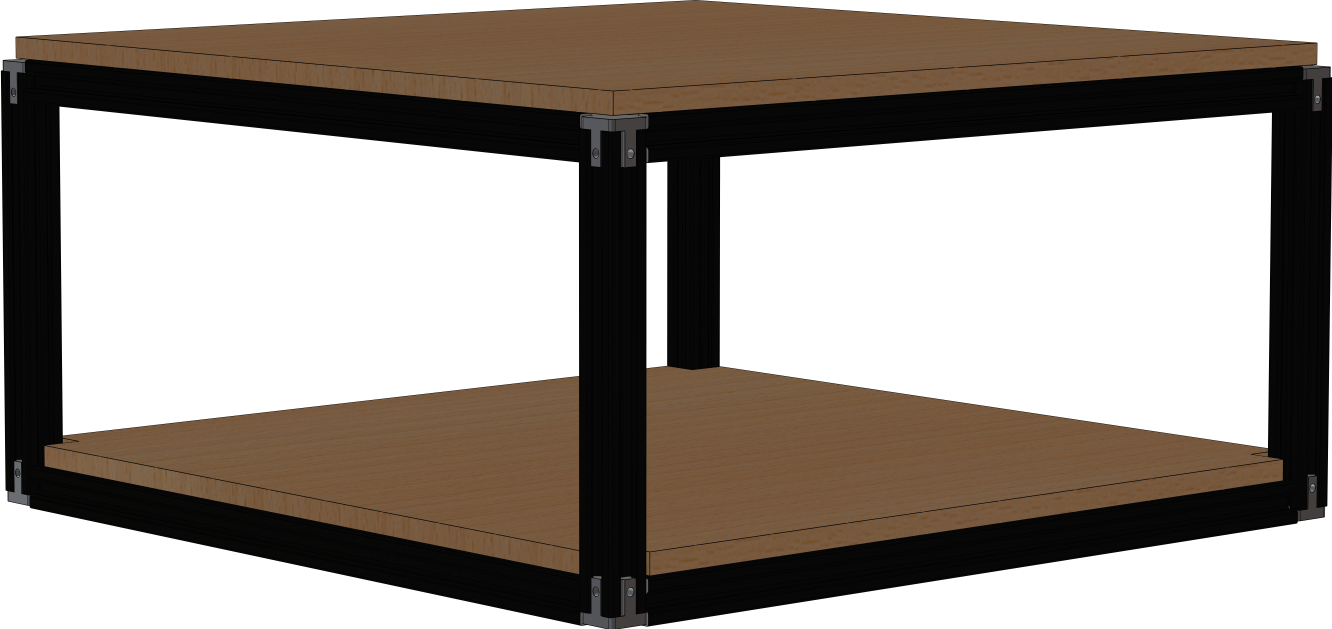
\includegraphics[width=\textwidth]{imgs/Chasis.png}
    \caption{Bare chassis}
    \label{fig:chassis_iso}
  \end{subfigure}

  \vspace{0em} % small gap between rows

  %--- Robot Views in 2×2 grid ---
  \begin{subfigure}[b]{0.3\textwidth}
    \centering
    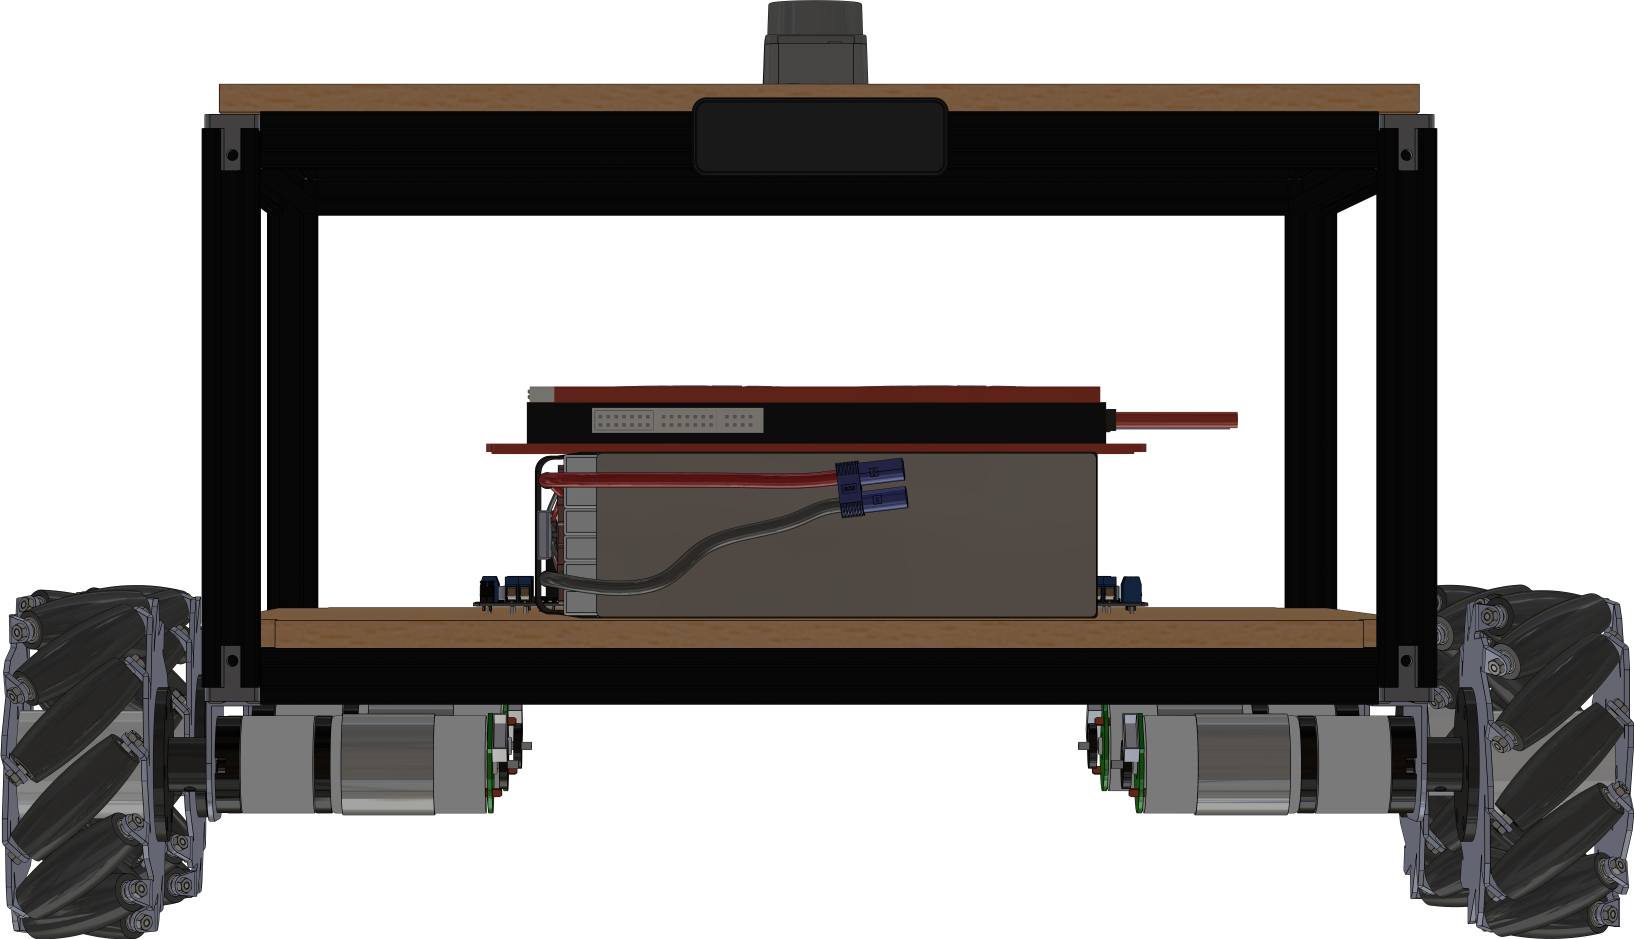
\includegraphics[width=\textwidth]{imgs/front.png}
    \caption{Front view}
    \label{fig:robot_front}
  \end{subfigure}
  \hfill
  \begin{subfigure}[b]{0.3\textwidth}
    \centering
    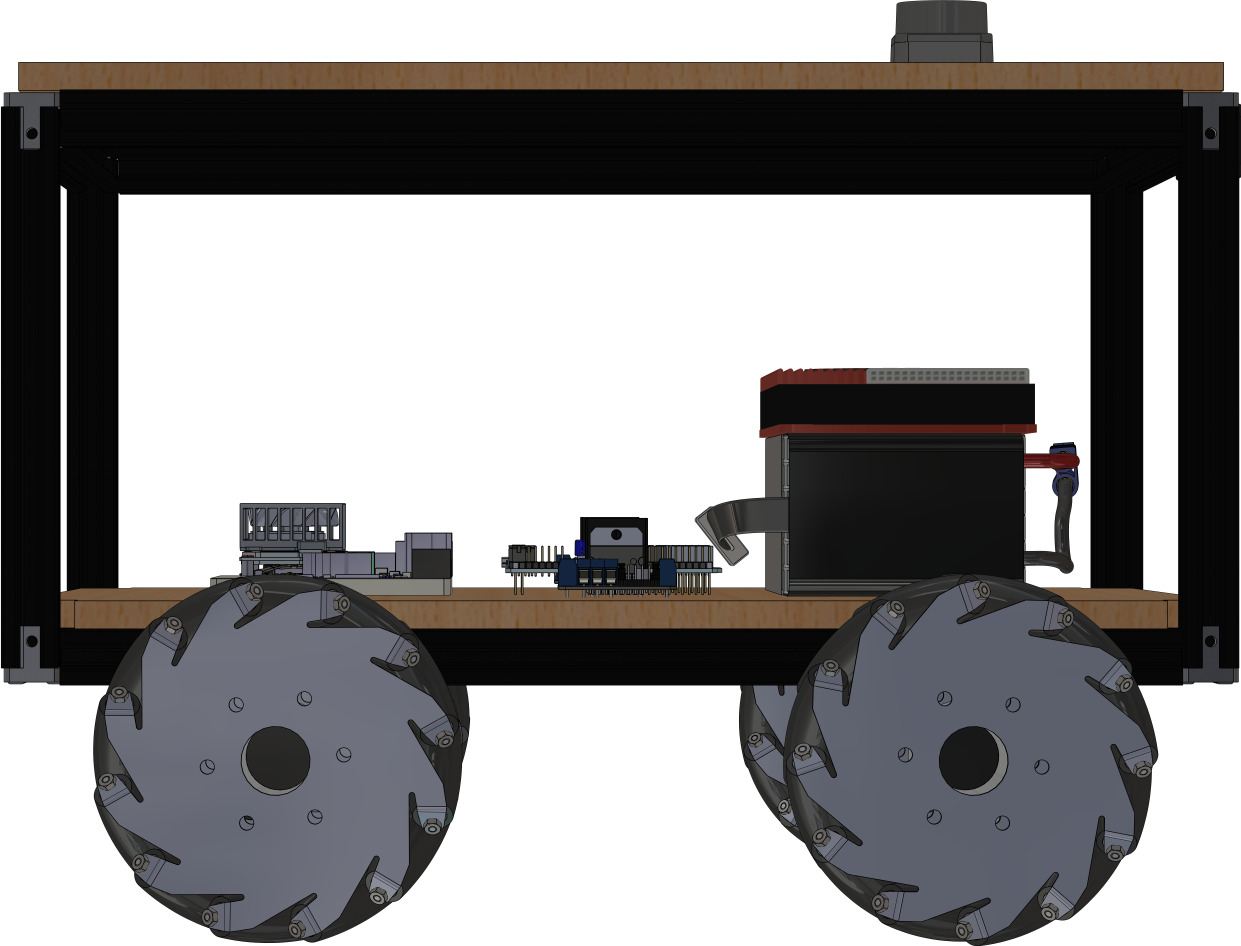
\includegraphics[width=\textwidth]{imgs/side.png}
    \caption{Side view}
    \label{fig:robot_side}
  \end{subfigure}

  \vspace{0em}

  \begin{subfigure}[b]{0.3\textwidth}
    \centering
    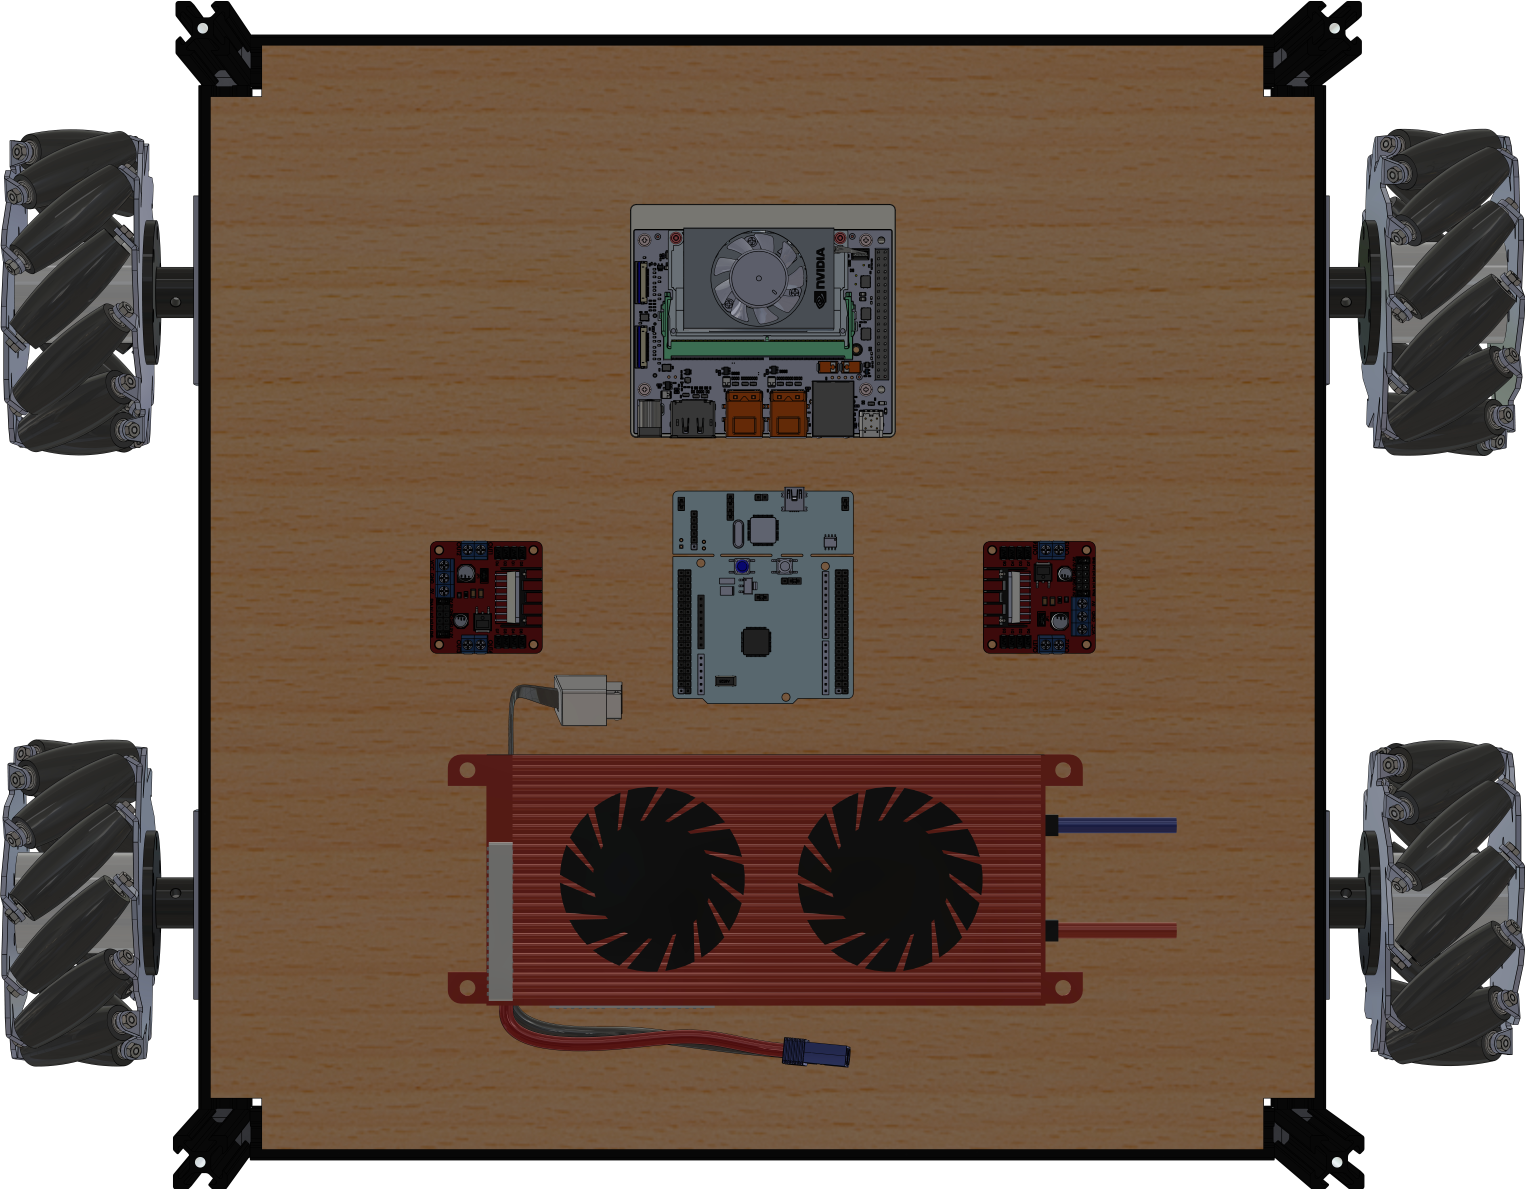
\includegraphics[width=\textwidth]{imgs/top.png}
    \caption{Top view}
    \label{fig:robot_top}
  \end{subfigure}
  \hfill
  \begin{subfigure}[b]{0.3\textwidth}
    \centering
    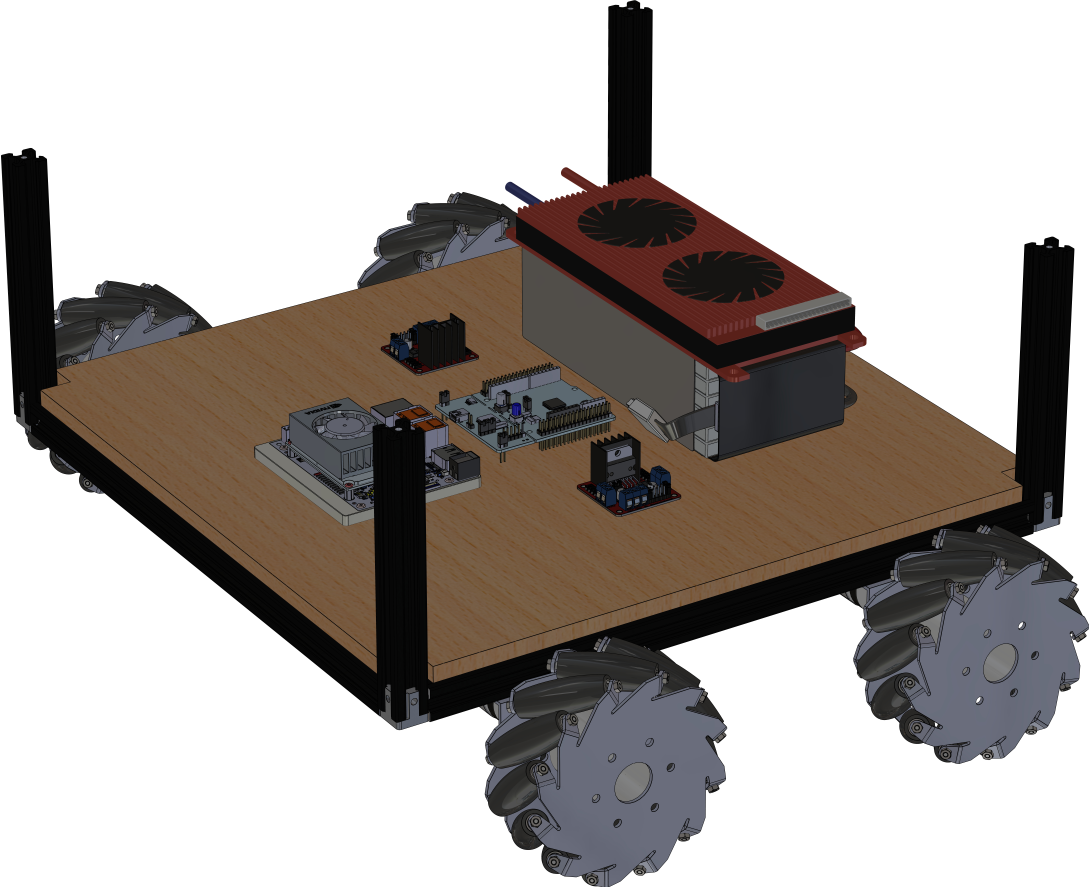
\includegraphics[width=\textwidth]{imgs/iso.png}
    \caption{Isometric view}
    \label{fig:robot_iso}
  \end{subfigure}

  \caption{%
    (a) Isometric view of the bare chassis,
    (b-e) Assembled robot with components: front, side, top, and isometric views
  }
  \label{fig:robot_overview}
\end{figure}


\section{Component layout}\label{sec:component_layout}

The internal arrangement of components has been chosen to optimize vehicle balance, minimize cable lengths, and ensure straightforward servicing. On the lower plywood shelf, the battery pack sits near the center of the robot. Placing the heaviest mass near the geometric center reduces pitch under acceleration or braking and maintains even weight distribution across all four wheels. Directly above the battery is the \gls{bms} allowing for the shortest cables for the many connections between them.
The \textbf{Jetson Orin Nano} is mounted at the back on the lower shelf, where its finned heat sink is free to draw air. The \gls{mcu} is placed at the geometrical center of the lower shelf, allowing for equal distance from all motors and drivers for better cable management. The motor driver boards are each positioned symmetrically between the corresponding wheel motors and close to the \gls{mcu}, shortening \gls{pwm} and \gls{hall} cable runs and improving signal integrity.
Above these power and compute elements, the \gls{lidar} sits near the front of the upper shelf. This placement is due to the improved construction of the environment when the \gls{lidar} is placed near the camera that is fixed with T-nuts on the upper V-slot of the frame.


\chapter{Development of the MCU}\label{chap:mcu}

This chapter details the development process of the firmware for an \textbf{STM32} \gls{mcu} tasked with controlling four DC motors. The system leverages \gls{hall} effect sensors for feedback, \gls{can} for communication, and \glspl{pid} for precise speed regulation. The following sections elaborate on the code structure, \gls{pid} design process, quadrature encoding, pin layout, and justifications for chosen methods.

\section{Hardware architecture}

\subsection{GPIO \& peripheral allocation}

The connections between the \gls{mcu} and the components are shown in table~\ref{tab:gpio-table} and \ref{tab:aux-peripherals}. The \gls{mcu} uses \gls{gpio} pins for motor control signals, \gls{hall} sensor inputs, and \gls{can} communication. The pin allocation is designed to minimize interference and ensure clear signal paths.

\begin{table}[H]
  \centering
  \sisetup{table-format=1.0}
  \begin{tabular}{@{}lll l l@{}}
    \toprule
    \textbf{Motor}                    & \textbf{Purpose} & \textbf{Pin} \\
    \midrule
    \multirow{3}{*}{Front-left (M1)}  & PWM (TIM1 CH1)   & PA8          \\
                                      & Dir A / Dir B    & PA0 / PA1    \\
                                      & Hall A / B       & PB6 / PB7    \\
    \midrule
    \multirow{3}{*}{Rear-left (M2)}   & PWM (TIM17 CH1)  & PB5          \\
                                      & Dir A / Dir B    & PB8 / PB9    \\
                                      & Hall A / B       & PA15 / PB3   \\
    \midrule
    \multirow{3}{*}{Front-right (M3)} & PWM (TIM16 CH1)  & PB4          \\
                                      & Dir A / Dir B    & PC6 / PC7    \\
                                      & Hall A / B       & PC12 / PD2   \\
    \midrule
    \multirow{3}{*}{Rear-right (M4)}  & PWM (TIM1 CH2)   & PA9          \\
                                      & Dir A / Dir B    & PB0 / PB1    \\
                                      & Hall A / B       & PC10 / PC11  \\
    \bottomrule
  \end{tabular}
  \caption{Pin allocation for power-stage control and sensing}
  \label{tab:gpio-table}
\end{table}

\begin{table}[H]
  \centering
  \begin{tabular}{@{}lll@{}}
    \toprule
    \textbf{Peripheral} & \textbf{Pins / Resources} & \textbf{Function}                       \\
    \midrule
    CAN1 (500 kbit/s)   & PA12 / PA11               & Real-time set-point \& feedback network \\
    TIM2                & Internal                  & 1 kHz scheduler and speed estimator     \\
    \bottomrule
  \end{tabular}
  \caption{Auxiliary peripheral allocation}
  \label{tab:aux-peripherals}
\end{table}


\subsection{Timer topology}

All \gls{pwm} generators share an identical base clock to guarantee phase coherence between wheels. With $PSC = 71$, the timer base frequency is \SI{1}{\MHz}; $ARR = 1999$ yields a \SI{500}{\Hz} \gls{pwm} frequency, fast enough for current control yet slow enough to avoid shoot through, also within the limits of the motor driver specifications.

\begin{table}[H]
  \centering
  \begin{tabular}{@{}llllll@{}}
    \toprule
    \textbf{Timer} & \textbf{Mode} & \textbf{PSC} & \textbf{ARR} & \textbf{IRQ}       & \textbf{Purpose}         \\
    \midrule
    TIM1           & PWM 1/2       & 71           & 1999         & -                  & Motors M1 \& M4          \\
    TIM16          & PWM 1         & 71           & 1999         & -                  & Motor M3                 \\
    TIM17          & PWM 1         & 71           & 1999         & -                  & Motor M2                 \\
    TIM2           & Up-counter    & 7199         & 9            & yes (\SI{1}{\kHz}) & Motion-control scheduler \\
    \bottomrule
  \end{tabular}
  \caption{Timer configuration}
\end{table}

\section{Software architecture}

\subsection{Modular design}

The firmware is organized as three cohesive modules mapping directly to the physical concerns of the traction subsystem: sensing, communication and control/actuation. Each module consists of header/implementation pairs. The \texttt{main.c} file handles initialization and scheduling.

\begin{table}[H]
  \centering
  \begin{tabular}{@{}llll@{}}
    \toprule
    \textbf{File / Module}      & \textbf{Layer} & \textbf{Core Responsibilities}               \\
    \midrule
    \texttt{main.c}             & Application    & Peripheral init                              \\
    \texttt{hall\_sensor.h/c}   & Sensing        & Quadrature decoding, speed estimation        \\
    \texttt{motor\_control.h/c} & Control        & PID, direction logic, PWM duty               \\
    \texttt{can.h/c}            & Communication  & Set-point \texttt{RX}, telemetry \texttt{TX} \\
    \bottomrule
  \end{tabular}
  \caption{Source file}
\end{table}

\subsection{Control-loop flow}

the \gls{mcu} starts with \texttt{HAL} initializing the timers, \gls{can} and data structures, where interrupt scheduler is sit for \texttt{TIM2} and a filter for the \gls{can}. After that, the control loop of the whole system starts simultaneously.

\subsubsection*{\texttt{hall\_sensor}}

The Hall Sensor Module implements quadrature decoding and speed filtering for up to four DC motors, each with a two-channel (A/B) \glspl{hall}. It comprises:

\begin{enumerate}
  \item \textbf{Data structures}
  \item \textbf{Real-time position update}
  \item \textbf{Speed computation and filtering}
  \item \textbf{API accessors}
\end{enumerate}

\paragraph*{Data structures}

The \texttt{MotorHallSensor} structure holds all necessary state for each motor, including position, speed, and \gls{gpio} handles. This design allows for efficient access when needed and manipulation of motor data. table~\ref{tab:motorhallsensor} summarizes the fields of the \texttt{MotorHallSensor} structure.
\begin{table}[H]
  \centering
  \begin{tabular}{@{}lll@{}}
    \toprule
    \textbf{Field}                     & \textbf{Type}                   & \textbf{Description}                  \\
    \midrule
    \texttt{last\_tick}                & \texttt{uint32\_t}              & Timestamp of last edge (ms)           \\
    \texttt{position}                  & \texttt{int32\_t}               & Cumulative quadrature-edge count      \\
    \texttt{direction}                 & \texttt{int8\_t}                & +1 or -1 for last movement            \\
    \texttt{prev\_ab\_state}           & \texttt{uint8\_t}               & Previous A/B logic state (0~\ldots~3) \\
    \texttt{portA}, \texttt{pinA}      & GPIO handle, \texttt{uint16\_t} & GPIO for channel A                    \\
    \texttt{portB}, \texttt{pinB}      & GPIO handle, \texttt{uint16\_t} & GPIO for channel B                    \\
    \texttt{accum\_counts}             & \texttt{uint32\_t}              & Pulses since last speed update        \\
    \texttt{ticks\_per\_sec\_computed} & \texttt{float}                  & Raw speed (ticks/s)                   \\
    \texttt{filtered\_ticks\_per\_sec} & \texttt{float}                  & Low-pass filtered speed               \\
    \texttt{reverse\_wiring}           & \texttt{bool}                   & Invert count if wiring flipped        \\
    \bottomrule
  \end{tabular}
  \caption{Fields of the \texttt{MotorHallSensor} data structure}
  \label{tab:motorhallsensor}
\end{table}



\paragraph*{Real-time position update}

To increase the precision of the position measurement beyond the native pulse count, a quadrature encoding scheme is employed. By sampling both channels A and B and decoding every valid transition, the effective ticks per mechanical revolution are doubled leading to 1728 ticks per second. in the figure~\ref{fig:quad} the quadrature encoder signals and edge counts are shown, where the resolution depends on if rising edges , falling edges or both are counted.

\begin{figure}[H]
  \centering
  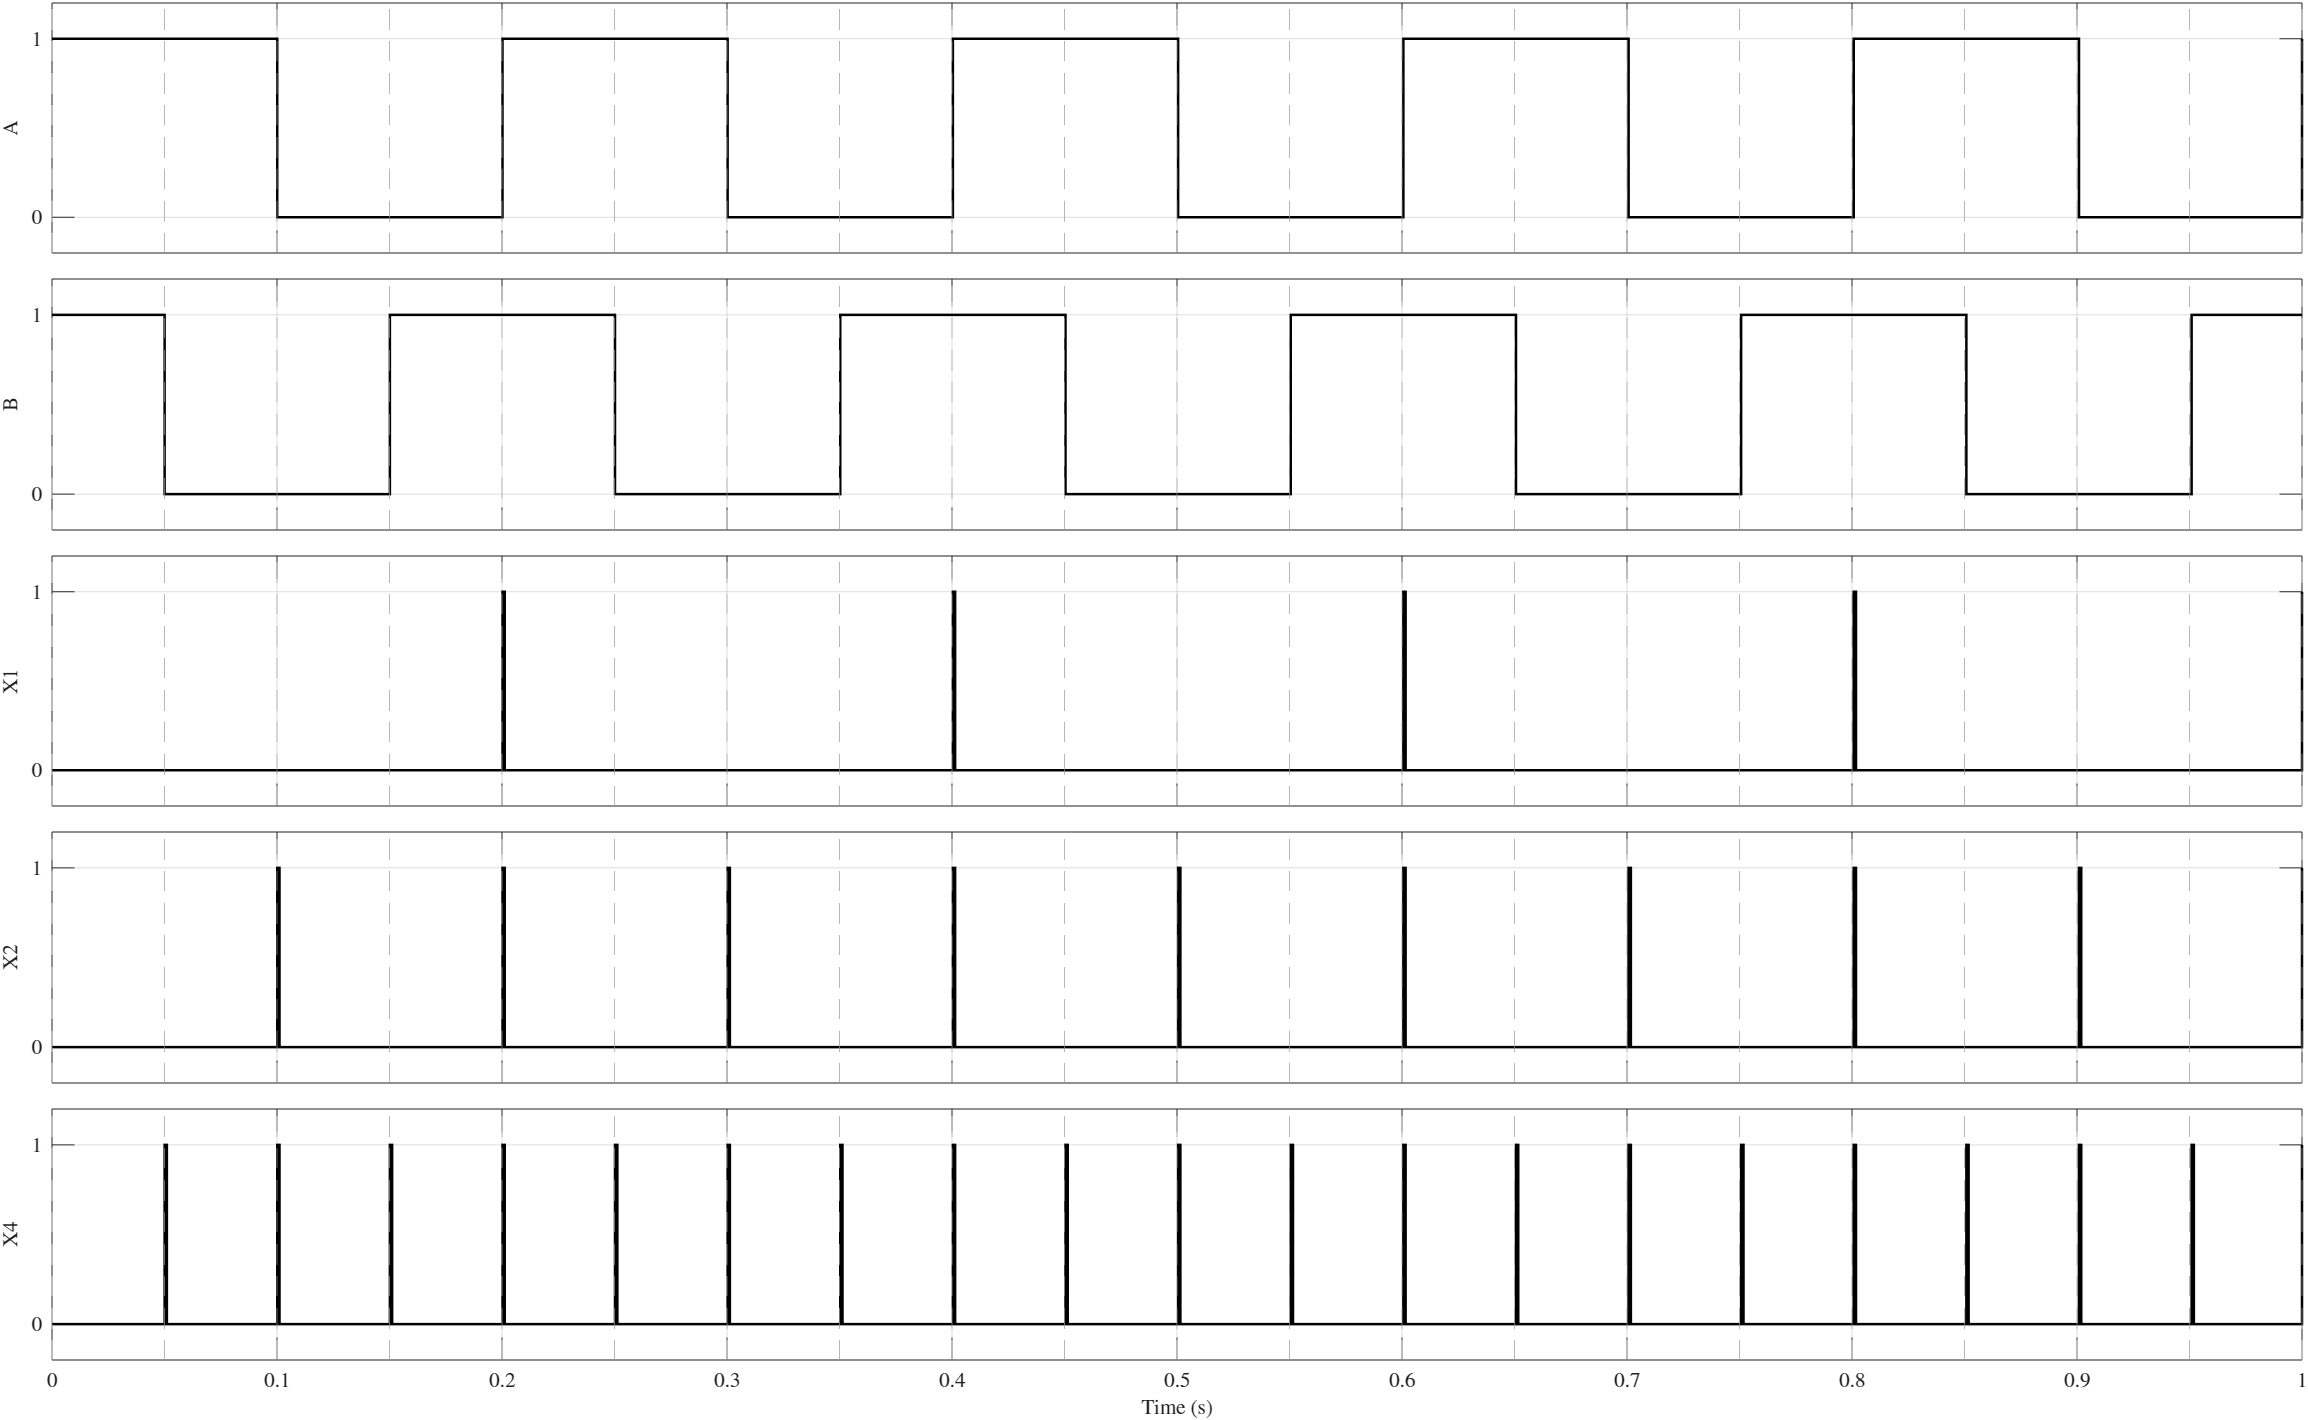
\includegraphics[width=0.5\textwidth]{imgs/quad.png}
  \caption{Quadrature encoder signals and edge counts}
  \label{fig:quad}
\end{figure}

\subparagraph*{Quadrature Encoding Mechanism}
A quadrature encoder produces two square-wave signals, A and B, ideally shifted in phase by \SI{90}{\degree}. At any instant the pair \((A,B)\) occupies one of four states:
\[
  \{00,\;01,\;11,\;10\},
\]
which is labeled in binary as \(0,1,2,3\).
Rather than using complex conditionals, an indexed 16-entry table is used by the concatenation \(\mathtt{idx} = (\text{prev\_ab\_state}\ll2)\,\vert\,(\text{curr\_ab\_state})\). Each entry returns \(\Delta~\!p\in\{-1,0,+1\}\), the signed increment in pulse count:

\[
  \mathtt{quad\_table}[\,(\,i\!\ll\!2)\mid j\,]
  =
  \begin{bmatrix}
    \;0 & +1  & -1  & \;0 \\
    -1  & \;0 & \;0 & +1  \\
    +1  & \;0 & \;0 & -1  \\
    \;0 & -1  & +1  & \;0
  \end{bmatrix}
  \quad
  \begin{aligned}
     & \text{prev}=00\;\big|\;\text{curr}=00,01,10,11 \\
     & \text{prev}=01\;\big|\;\text{curr}=00,01,10,11 \\
     & \text{prev}=10\;\big|\;\text{curr}=00,01,10,11 \\
     & \text{prev}=11\;\big|\;\text{curr}=00,01,10,11
  \end{aligned}
\]

Illegal transitions (e.g.\ jumping from 00 directly to 11) map to zero, enabling robust error detection in the presence of noise or missed edges.
in the algorithm~\ref{alg:update_motor_position} the quadrature encoding is implemented, where the \texttt{motor.read\_A()} and \texttt{motor.read\_B()} functions read the current state of the \gls{hall} sensors, and the \texttt{quad\_table} is used to determine the change in position based on the previous and current states.
\begin{algorithm}[H]
  \caption{update\_motor\_position}
  \begin{algorithmic}[1]
    \Function{update\_motor\_position}{$motors, quad\_table$}
    \ForAll{motor \textbf{in} motors}
    \State $A \gets \text{motor.read\_A}()$
    \State $B \gets \text{motor.read\_B}()$
    \State $state \gets B\ll1~| A$
    \If{$state \neq \text{motor.prev\_state}$}
    \State $idx \gets \text{motor.prev\_state}\ll2~| state$
    \State $delta \gets \text{quad\_table}[idx]$
    \If{$delta \neq 0$}
    \If{$\text{motor.reverse\_wiring}$}
    \State $delta \gets -\,delta$
    \EndIf
    \State $\text{motor.position} \gets \text{motor.position} + delta$
    \State $\text{motor.direction} \gets \text{sign}(delta)$
    \State $\text{motor.counts} \gets \text{motor.counts} + delta$
    \EndIf
    \State $\text{motor.prev\_state} \gets state$
    \EndIf
    \EndFor
    \EndFunction
  \end{algorithmic}
  \label{alg:update_motor_position}
\end{algorithm}

\paragraph*{Speed computation and filtering}

The linear velocity of each motor is computed at a fixed update rate (via a timer interrupt at frequency \(f_{TIM_2}\)). During each interval, the number of quadrature counts accumulated, \(\Delta c\), is converted into speed in ticks per second:
\begin{equation}
  \upsilon \;=\; \Delta c \;\times\; f_{\text{upd}}.
\end{equation}
Immediately after computing \(\upsilon\), the accumulator \(\Delta c\) is reset to zero for the next interval. To reduce measurement noise, an exponential (first-order low-pass) filter is applied:
\begin{equation}
  \upsilon_{\text{filt}} \;=\; \alpha\,\upsilon_{\text{filt,prev}}
  \;+\;(1-\alpha)\,\upsilon_{\text{raw}},
\end{equation}
where \(0<\alpha<1\) is the filter coefficient.

\begin{algorithm}[H]
  \caption{compute\_speed\_for\_all\_motors}
  \begin{algorithmic}[1]
    \Function{compute\_speed\_for\_all\_motors}{$motors, \alpha, f_{TIM_2}$}
    \ForAll{motor \textbf{in} motors}
    \State \(\upsilon \gets \text{motor.counts} \;\times\; f_{TIM_2}\)
    \State $\text{motor.counts} \gets 0$
    \State \texttt{motor.filtered\_speed}$ \gets \alpha \cdot$ \texttt{motor.filtered\_speed} $+ (1 - \alpha) \cdot \upsilon$
    \EndFor
    \EndFunction
  \end{algorithmic}
\end{algorithm}

\paragraph*{Sensor Data Access API}

To expose the encoder measurements to higher-level control routines, three accessor functions are provided. Each takes an integer identifier \(i\) (with \(1\le i\le N\), where \(N\) is the number of motors) and returns the corresponding data, or zero if \(i\) is out of range.

\begin{algorithm}[H]
  \caption{motor\_API}
  \begin{algorithmic}[1]
    \State \textbf{function} get\_motor\_position($motors, i$)
    \If{$1 \le i \le |\text{motors}|$}
    \State \Return motors[$i$].position
    \Else
    \State \Return $0$
    \EndIf
    \State \textbf{end function}
    \State \textbf{function} get\_motor\_direction($motors, i$)
    \Comment{Same process as the previous}
    \State \textbf{function} get\_motor\_speed($motors, i$)
    \Comment{Same process as the previous}
  \end{algorithmic}
\end{algorithm}
%% ----------------------------------------------------------------
%% Subsubsection: motor_control 
%% ----------------------------------------------------------------
\subsubsection*{\texttt{motor\_control}}\label{sec:motor_control}

The Motor Control module was implemented to control the four motors dynamically through a closed-loop system with a \gls{pid} for each motor.

%% ----------------------------------------------------------------
\paragraph*{System Modeling and Identification}
To characterize each motor, a PWM step input (12.5\%$\rightarrow$25\%) was applied~\footnote{The initial duty cycle was set above $0\%$ to avoid the starting voltage and static friction.}, and the speed response (ticks/s) was recorded by connecting the \gls{can} to Matlab. The procedure was as follows:
\begin{enumerate}
  \item Filter the measured signal using a 5-sample moving average
  \item Create an \texttt{iddata} object in MATLAB
  \item Estimate a second order model with \texttt{System identification} tool~\footnote{Second order models were chosen to capture the dynamics of the motors, which typically exhibit a second order response due to inertia and damping.}.
\end{enumerate}

The open-loop system response can be observed in Figure~\ref{fig:openloopres}.

\begin{figure}[H]
  \centering
  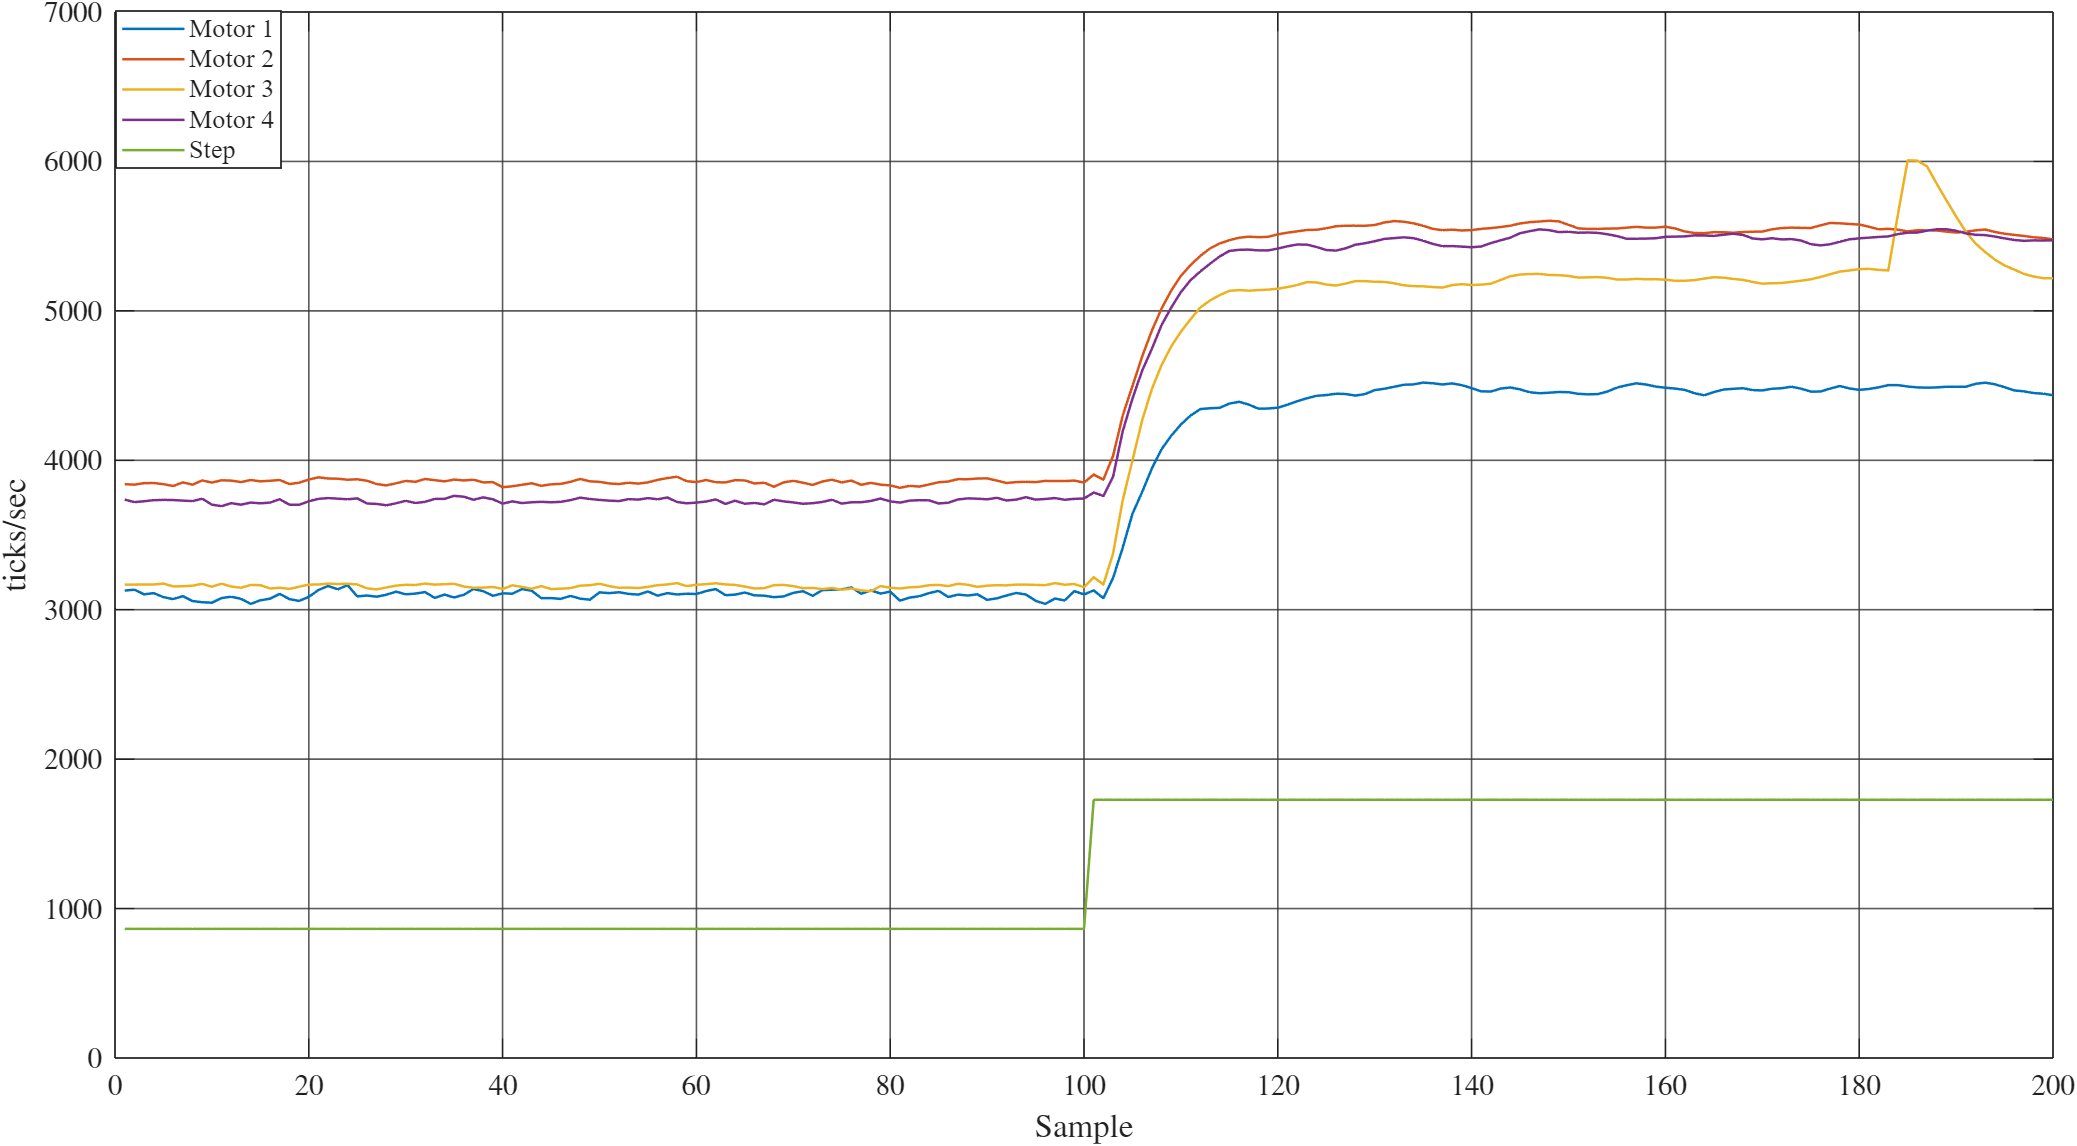
\includegraphics[width=0.85\textwidth]{imgs/openloopres.png}
  \caption{Open-loop response of the four motors to step input}
  \label{fig:openloopres}
\end{figure}

The identified transfer functions are summarized in Table~\ref{tab:identification}~\footnote{Motors typically exhibit a pole at the origin in their transfer function due to the integration of velocity to obtain position. This reflects the physical reality that, in the absence of feedback, a constant input results in continuous motion.}.

\begin{table}[H]
  \centering
  \begin{tabular}{@{}llll@{}}
    \toprule
    \textbf{Motor}   & \textbf{Poles} & \textbf{Zeros} \\
    \midrule
    \texttt{Motor 1} & -1.70 \& 0     & -0.005         \\
    \texttt{Motor 2} & -1.67 \& 0     & 0.005          \\
    \texttt{Motor 3} & -2.37 \& 0     & -0.03          \\
    \texttt{Motor 4} & -1.66 \& 0     & 0.001          \\
    \bottomrule
  \end{tabular}
  \caption{Identified poles and zeros for the four motors}
  \label{tab:identification}
\end{table}

%% ----------------------------------------------------------------
\paragraph*{PID Controller Design and Tuning}
Using MATLAB's Control System Toolbox, a settling time of $2~sec$ and high robustness was demanded, and a \gls{pid} was designed for each motor model,
The resulting \glspl{pid} parameters are listed in Table~\ref{tab:pid_constants}.

\begin{table}[H]
  \centering
  \begin{tabular}{@{}lccc@{}}
    \toprule
    \textbf{Motor} & $K_p$  & $T_i$ [s] & $T_d$ [s] \\
    \midrule
    \texttt{M1}    & 0.3620 & 0.5902    & 0.0001    \\
    \texttt{M2}    & 0.2540 & 0.4720    & 0.0001    \\
    \texttt{M3}    & 0.1633 & 0.4193    & 0.0001    \\
    \texttt{M4}    & 0.2120 & 0.5030    & 0.0001    \\
    \bottomrule
  \end{tabular}
  \caption{PID parameters obtained}
  \label{tab:pid_constants}
\end{table}


Figure~\ref{fig:step_responses} shows the closed-loop step responses for all four motors using the tuned PID controllers.

\begin{figure}[H]
  \centering
  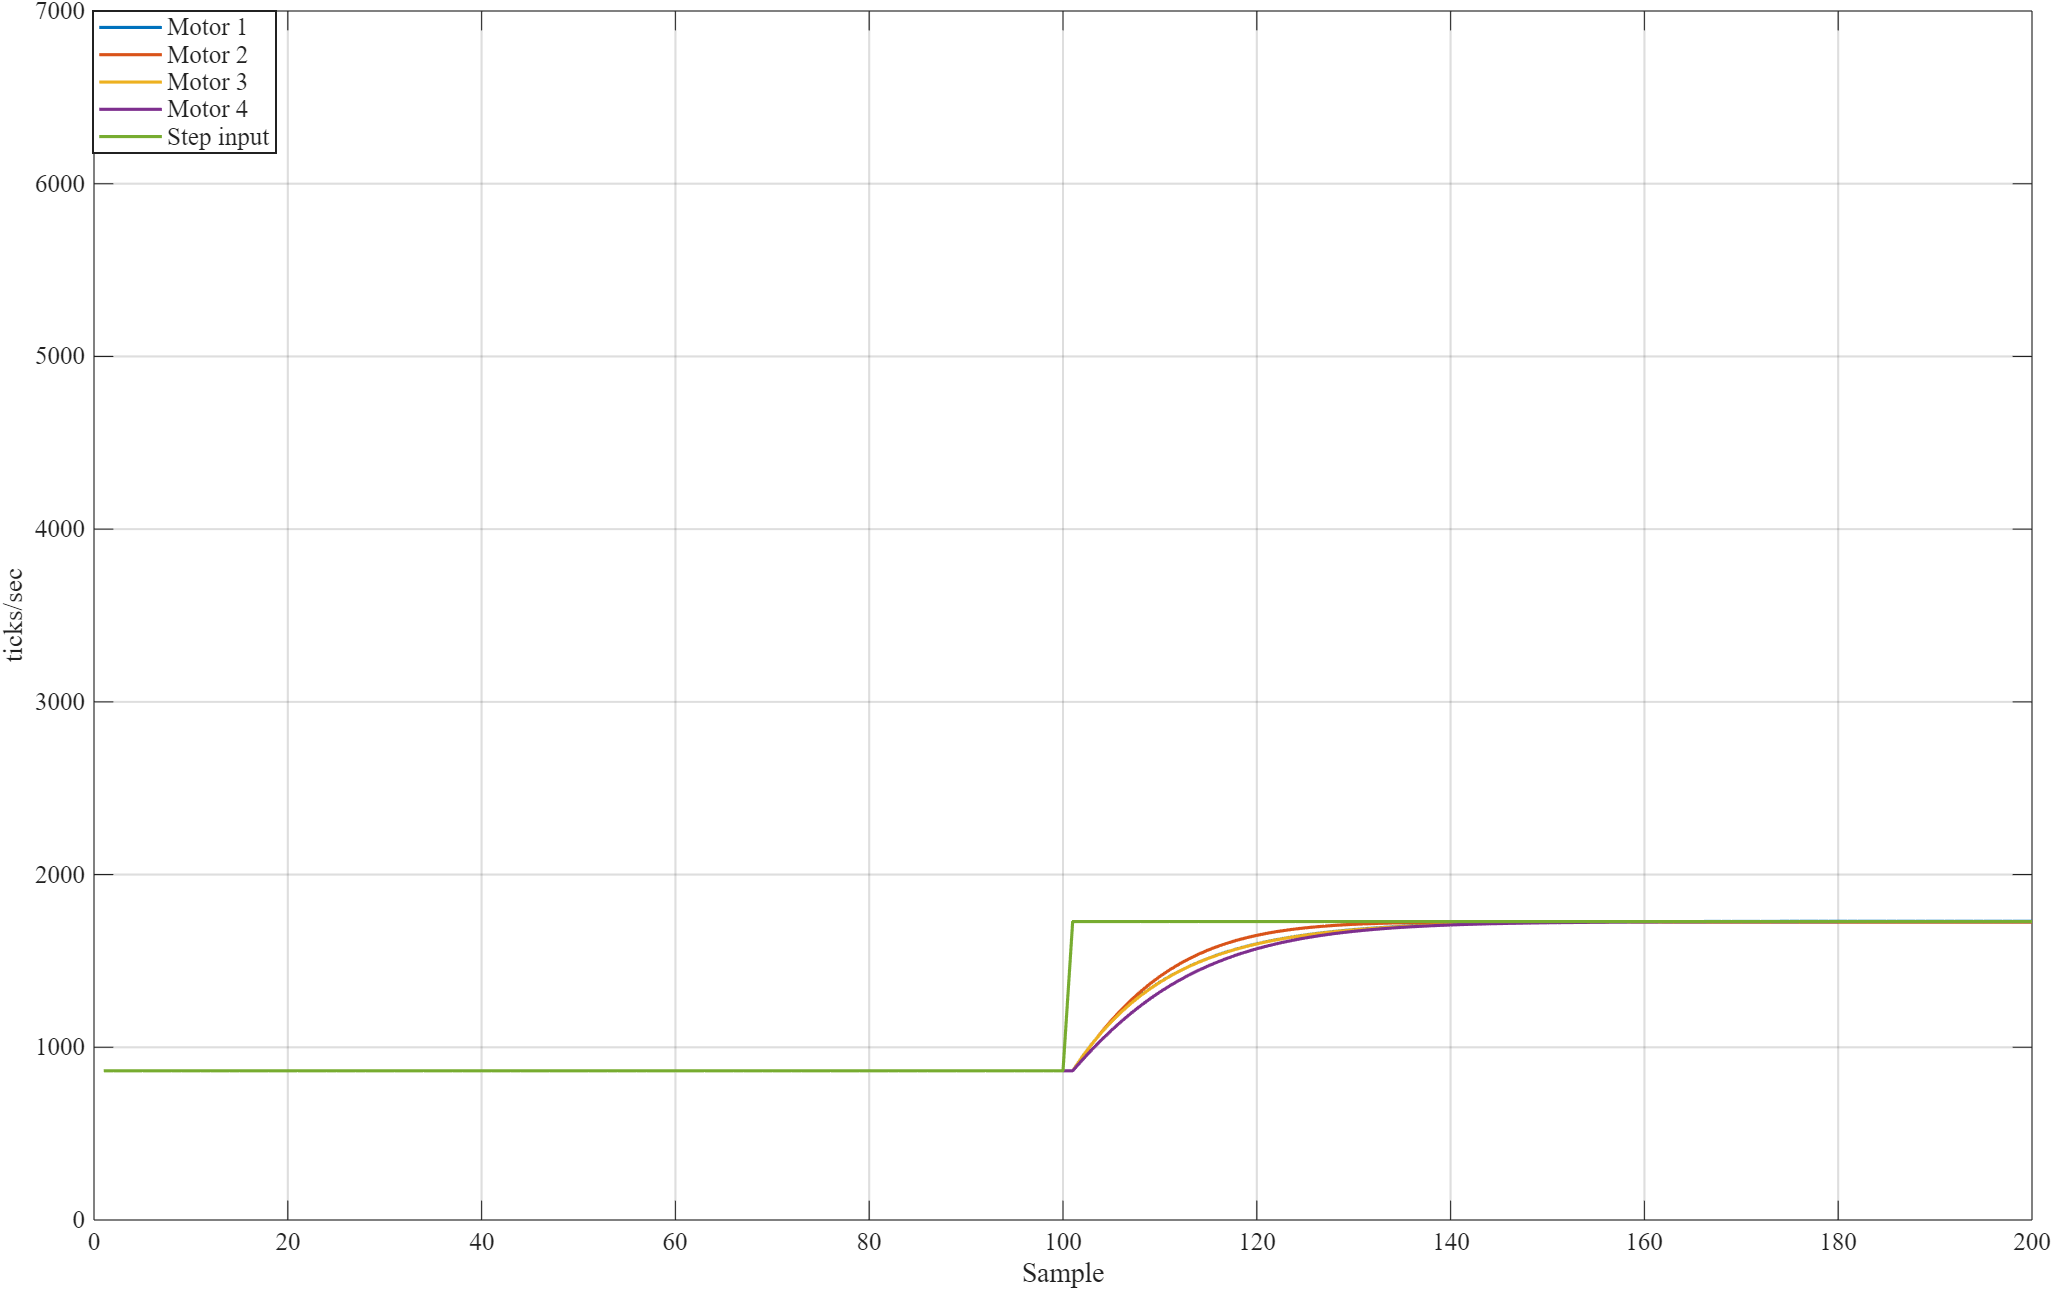
\includegraphics[width=0.85\textwidth]{imgs/closed res.png}
  \caption{Closed-loop step responses for each motor with tuned PID controllers}
  \label{fig:step_responses}
\end{figure}

%% ----------------------------------------------------------------
\paragraph*{Real-time Implementation}
The implemented discrete time \gls{pid} equation is:
\begin{equation}
  u[t] = K_p e[t] + K_p \frac{T_s}{T_i} \sum_{i=0}^{t} e[i] + K_p \frac{T_d}{T_s}\bigl(e[t] - e[t-1]\bigr).
\end{equation}
It runs every $\Delta t = $\SI{10}{\milli\second} in a \texttt{TIM2} interrupt, where the integration error is reset every \SI{100}{\milli\second}, and the output is scaled to \gls{pwm}:
\begin{equation}
  \mathrm{duty} = \mathrm{clamp}\Bigl(\frac{|u[k]|}{MAX\sfrac{TICKS}{SEC}} \cdot DUTY\_MAX\Bigr).
\end{equation}

Direction control is done based on the sign of $u[k]$ (via \texttt{set\_motor\_direction}).

%% ----------------------------------------------------------------
\subsubsection*{\texttt{can}}\label{sec:can}

The \gls{can} communication module controls the bidirectional setpoint/feedback exchange with the \texttt{Jetson}.

\paragraph*{CAN Message Reception}
Incoming frames are parsed into four signed 16-bit setpoints (\(fl,fr,rl,rr\)) as shown in Algorithm~\ref{alg:can_rx}.

\begin{algorithm}[H]
  \caption{receive\_can\_rx}
  \begin{algorithmic}[1]
    \Function{parse\_can\_rx}{$RxHeader, RxData$}
    \State \(\text{Receive CAN message into }RxData[8]\)
    \State \(fl \gets \text{int16}(RxData[0]\ll8 \mid RxData[1])\)
    \State \(fr \gets \text{int16}(RxData[2]\ll8 \mid RxData[3])\)
    \State \(rl \gets \text{int16}(RxData[4]\ll8 \mid RxData[5])\)
    \State \(rr \gets \text{int16}(RxData[6]\ll8 \mid RxData[7])\)
    \EndFunction
  \end{algorithmic}
  \label{alg:can_rx}
\end{algorithm}

\paragraph*{CAN Message Transmission}
Motor positions are read, packed into an 8-byte payload, and sent with an extended ID. Payload layout is shown in Table~\ref{tab:can_txdata}. The algorithm~\ref{alg:send_can_tx} is called periodically in the \texttt{TIM2} interrupt to transmit the current motor positions.

\begin{table}[H]
  \centering
  \begin{tabular}{c|c|c}
    \hline
    Bytes           & Field   \\
    \hline
    \texttt{[0--1]} & pos1 M1 \\
    \texttt{[2--3]} & pos2 M2 \\
    \texttt{[4--5]} & pos3 M3 \\
    \texttt{[6--7]} & pos4 M4 \\
    \hline
  \end{tabular}
  \caption{\texttt{TX} Data byte mapping for motor positions}
  \label{tab:can_txdata}
\end{table}

\begin{algorithm}[H]
  \caption{send\_can\_tx}
  \begin{algorithmic}[1]
    \Function{send\_can\_tx}{}
    \State \(pos1 \gets \text{get\_motor\_position}(1)\)
    \State \(pos2 \gets \text{get\_motor\_position}(2)\)
    \State \(pos3 \gets \text{get\_motor\_position}(3)\)
    \State \(pos4 \gets \text{get\_motor\_position}(4)\)
    \For{\(i = 0\) to \(3\)}
    \State \(TxData[2i]  \gets \text{MSB of }pos_{i+1}\)
    \State \(TxData[2i+1] \gets \text{LSB of }pos_{i+1}\)
    \EndFor
    \State \(\text{Transmit }TxData\) with extended ID
    \EndFunction
  \end{algorithmic}
  \label{alg:send_can_tx}
\end{algorithm}

\section{Optimization}

To maximize real-time performance and minimize \gls{cpu} load on the \gls{mcu}, several low-level optimizations were applied throughout the firmware. These focus on reducing instruction overhead, avoiding dynamic control constructs where feasible, and minimizing interrupt contention. The key strategies are outlined below:

\begin{description}[font=\normalfont\bfseries,leftmargin=!,labelwidth=\widthof{\bfseries Loop Unrolling}]
  \item[Direct register access vs.\ HAL]
        In timing-critical paths, peripheral registers are written directly rather than via higher-level HAL calls. This bypasses function call overhead and eliminates extra layers of abstraction, improving response time by tens of instruction cycles. In less critical sections, the HAL API remains for readability and maintainability.

  \item[Interrupt driven processing]   A hybrid approach uses dedicated interrupts to guarantee deterministic execution of the control loop and message handling. High rate \gls{hall} edges, however, are processed in the main loop rather than via interrupts preventing queue overflow due to their high frequency.

  \item[Pointer utilization for data structures]
        Motor and sensor data are stored in contiguous arrays of structures, accessed by pointers in control and sensing routines. This eliminates repeated index arithmetic and enables the compiler to perform prefetch optimizations.

  \item[Loop unrolling]
        All loops have been manually unrolled. By reducing branch and loop-control instructions, these routines execute in fewer cycles.

  \item[Use of \texttt{inline} and \texttt{static} Functions]
        Small, frequently invoked helpers are declared as \texttt{static inline}. This gives them internal linkage (so they can be discarded if unused) and encourages the compiler to expand them at call sites eliminating call/return overhead.
\end{description}

\chapter{Development of the ROS~2 workspace}\label{chap:ros2}

This chapter describes how \gls{ros} was used to implement the core functionality of the mobile robotics system motivating the environment setup, system design, node implementation and launch orchestration.

\section{Development environment}

When selecting the environment, the focus was on working with new versions that have \gls{lts} that allows the project to be used for more time without the necessity to change the source code, also, having community's developed tools and support.
considering the \gls{ros} version, \gls{ros}~2 have been chosen since it is the latest version, and new tools and algorithms are being introduced periodically, while \gls{ros} 1 has lost its support. The \texttt{Humble Hawksbill} distribution also have been used for the same reasons, adding to that its stability over other distributions.
These two middleware show high compatibility with \textbf{Jetson's} software (\texttt{ubuntu 22.04} and \texttt{Jetpack 6}).
From the \gls{ros} community packages, three packages have been used to help with the construction and simulation of the robot
\begin{itemize}
  \item \textbf{RViz} which is 3D visualizer for the \gls{ros} framework. This will helps visualize the data, map and robots position during testing and execution.

  \item \textbf{Nav2} which is a navigation stack for the \gls{ros} framework. It helps generating the \gls{costmap} and translate movement planning into logical steps~\cite{nav2}.

  \item \textbf{SLAM Toolbox} which is a toolbox that includes the \gls{slam} algorithms for direct configuration and implantation~\cite{slamtool}.
\end{itemize}

\section{Nodes structure}

the system composes of seven main nodes

\begin{enumerate}

  \item Camera

  \item \gls{lidar}

  \item \gls{can} communication

  \item Motor control

  \item Odometry

  \item \gls{rtab}

  \item Nav2

\end{enumerate}

On top of the Rviz2 Node for visualizing.

\subsection{Camera node}

The camera node is responsible for interfacing the DepthAI \textbf{Oak-D} camera with the \gls{ros}~2 ecosystem. It encapsulates device discovery and connection, image acquisition and publishing, dynamic reconfiguration of camera parameters, and provision of auxiliary services for operational control and data dumping. The implementation follows a modular, parameter-driven design, as described below~\cite{cameranode}.

The DepthAI pipeline is wrapped by a corresponding \gls{ros}~2 bridge object which establishes asynchronous queues for image and metadata transport. The camera node iterates over these bridge objects to call \texttt{setupQueues()}, ensuring raw images, camera calibration information and any outputs are published on standard \gls{ros} topics~\footnote{The fabricant provides the calibration matrix that when tested proved to be accurate, therefore, it is used as is.}. The pipeline establishes \glspl{tf} between the lenses, mainly for 3D construction of images.

\paragraph*{TF frames}
\begin{table}[H]
  \centering
  \begin{tabularx}{\textwidth}{ll}
    \toprule
    \textbf{Frame} & \textbf{Description}                                 \\
    \midrule
    \texttt{<base\_link> $\rightarrow$ <camera\_frame>}
                   & Static transform base link to optical center         \\
    \texttt{<camera\_frame> $\rightarrow$ <center\_optical\_frame>}
                   & Static transform optical axis frame to RGB lens      \\
    \texttt{<camera\_frame> $\rightarrow$ <right/left\_optical\_frame>}
                   & Static transform optical axis frame to stereo lenses \\
    \bottomrule
  \end{tabularx}
  \caption{TF frames broadcast by the camera node}
  \label{tab:camera-tf-frames}
\end{table}

\paragraph*{ROS\,2 topics}
\begin{table}[H]
  \centering
  \begin{tabular}{lll}
    \toprule
    \textbf{Topic}                   & \textbf{Type} & \textbf{Description}            \\
    \midrule
    \texttt{/oak/rgb/image\_raw}     & Publication   & Raw RGB image stream            \\
    \texttt{/oak/stereo/image\_rect} & Publication   & Depth image aligned to RGB      \\
    \texttt{/oak/rgb/camera\_info}   & Publication   & Intrinsics for the color camera \\
    \bottomrule
  \end{tabular}
  \caption{ROS\,2 topics used by the camera node}
  \label{tab:camera-topics}
\end{table}

\subsection{LiDAR node}

The \gls{lidar} node is responsible for interfacing the \textbf{ld19} \gls{lidar} with the \gls{ros}~2 ecosystem. It handles serial port discovery and connection, continuous acquisition of 2D scan data, and conversion into standard \gls{ros}~2 messages.~\cite{ldlidar}. The implementation uses the \texttt{LDLiDAR} Linux Interface driver and converts raw polar scan points into Cartesian point clouds on the fly.

\paragraph*{TF frames}

\begin{table}[H]
  \centering
  \begin{tabular}{ll}
    \toprule
    \textbf{Frame}                                    & \textbf{Description}                           \\
    \midrule
    \texttt{<base\_link> $\rightarrow$ <base\_laser>} & Static transform from base link to laser base. \\
    \bottomrule
  \end{tabular}
  \caption{TF frames broadcast by the LiDAR node}
  \label{tab:ldlidar-tf-frames}
\end{table}

\paragraph*{ROS\,2 topics}
\begin{table}[H]
  \centering
  \begin{tabular}{lll}
    \toprule
    \textbf{Topic}                   & \textbf{Type}                             & \textbf{Description} \\
    \midrule
    \texttt{/lidar/laser\_scan}      & Publication
                                     & 2D laser scan: ranges + intensities.                             \\
    \texttt{/lidar/point\_cloud\_2d} & Publication
                                     & 2D point cloud: Cartesian XY + intensity.                        \\
    \bottomrule
  \end{tabular}
  \caption{ROS 2 topics used by the Lidar node}
  \label{tab:ldlidar-topics}
\end{table}


\subsection{CAN node}

The \gls{can} node interfaces the vehicle's wheel control and feedback mechanism with the \gls{ros}~2 ecosystem via a \gls{can} bus. It subscribes to the \texttt{wheels\_desired\_rate} topic to receive four signed 16-bit desired wheel speeds, buffers them, and transmits them as an extended-ID \gls{can} frame at 10 Hz. Concurrently, it listens for incoming \gls{can} frames on a configurable ID, parses four signed 16-bit wheel encoder ticks, and republishes them on the \texttt{wheel\_ticks} topic as an \texttt{Int16MultiArray}. All behavior (\gls{can} interface name, transmit/receive IDs, and incoming frame filtering) is driven by \gls{ros}~2 parameters.

\paragraph*{ROS\,2 topics}
\begin{table}[H]
  \centering
  \begin{tabular}{lll}
    \toprule
    \textbf{Topic}                  & \textbf{Type}                                                      & \textbf{Description} \\
    \midrule
    \texttt{/wheels\_desired\_rate} & Subscription
                                    & Desired wheel speeds (\texttt{Int16MultiArray}, 4 elements).                              \\
    \texttt{/wheel\_ticks}          & Publication
                                    & Actual wheel encoder ticks (\texttt{Int16MultiArray}, 4 elements).                        \\
    \bottomrule
  \end{tabular}
  \caption{ROS\,2 topics used by the CAN node}
  \label{tab:can-topics}
\end{table}

\subsection{Odometry node}

The Odometry node computes the robot's planar pose and velocity by integrating wheel encoder ticks acquired through the \gls{can}. Upon startup, the node configures an internal \texttt{Odometry} object. At a fixed rate it executes the following odometry update routine:

First, each wheel's encoder instance reports the delta ticks $\Delta n_*$ since the previous cycle (handling 16-bit overflow). These are converted into linear wheel travels:
\begin{equation}
  d_* \;=\; \frac{\Delta n_*}{\mathtt{ticks\_per\_meter}}
\end{equation}

Next, the standard mecanum kinematic model computes the body frame displacements and rotation increment:

\begin{equation}
  \begin{aligned}
    \Delta x_r
     & = \frac{d_{\mathrm{fl}} + d_{\mathrm{fr}} + d_{\mathrm{rl}} + d_{\mathrm{rr}}}{4},    \\
    \Delta y_r
     & = \frac{-\,d_{\mathrm{fl}} + d_{\mathrm{fr}} + d_{\mathrm{rl}} - d_{\mathrm{rr}}}{4}, \\
    \Delta\theta
     & = \frac{-\,d_{\mathrm{fl}} + d_{\mathrm{fr}} - d_{\mathrm{rl}} + d_{\mathrm{rr}}}
    {2\,(L_w + L_\ell)}.
  \end{aligned}
\end{equation}

These local displacements are then rotated into the global \texttt{odom} by the previous yaw $\theta_{t-1}$:
\begin{equation}
  \begin{aligned}
    \Delta x & = \Delta x_r\cos\theta_{t-1} \;-\; \Delta y_r\sin\theta_{t-1}, \\
    \Delta y & = \Delta x_r\sin\theta_{t-1} \;+\; \Delta y_r\cos\theta_{t-1}.
  \end{aligned}
\end{equation}

The node updates its pose:
\begin{equation}
  \begin{aligned}
    x_t      & = x_{t-1} + \Delta x,          \\
    y_t      & = y_{t-1} + \Delta y,          \\
    \theta_t & = \theta_{t-1} + \Delta\theta,
  \end{aligned}
\end{equation}

\paragraph*{TF frames}
\begin{table}[H]
  \centering
  \begin{tabularx}{\textwidth}{ll}
    \toprule
    \textbf{Frame} & \textbf{Description}                                     \\
    \midrule
    \texttt{<odom\_frame> $\rightarrow$ <base\_frame>}
                   & Dynamic transform from odometry frame to robot base link \\
    \bottomrule
  \end{tabularx}
  {TF frames broadcast by the Odometry node}
  \label{tab:odo-tf-frames}
\end{table}

\paragraph*{ROS\,2 topics}
\begin{table}[H]
  \centering
  \begin{tabular}{lll}
    \toprule
    \textbf{Topic}         & \textbf{Type}                                                & \textbf{Description} \\
    \midrule
    \texttt{/wheel\_ticks} & Subscription
                           & Encoder ticks (\texttt{Int16MultiArray} coming from CAN bus)                        \\
    \texttt{/odom}         & Publication
                           & Computed odometry                                                                   \\
    \bottomrule
  \end{tabular}
  \caption{ROS\,2 topics used by the Odometry node}
  \label{tab:odo-topics}
\end{table}

\begin{algorithm}[H]
  \caption{update\_mecanum\_odometry}
  \begin{algorithmic}[1]
    \Function{update\_mecanum\_odometry}{$\Delta n_{*}, \nicefrac{ticks}{meter}, L_w, L_\ell,$}
    \State $d_{*} \gets \Delta n_{*} / \nicefrac{ticks}{meter}$
    \State $\Delta x_r \gets (d_{rr} + d_{rl} + d_{fr} + d_{fl}) / 4$
    \State $\Delta y_r \gets (-d_{rr} + d_{rl} + d_{fr} - d_{fl}) / 4$
    \State $\Delta \theta \gets (-d_{rr} + d_{rl} - d_{fr} + d_{fl}) \,/\, \bigl(2\,(L_w + L_\ell)\bigr)$
    \State $\theta_{t} \gets \theta_{t-1} + \Delta \theta$
    \State $x_{t} \gets x_{t-1} + \Delta x_r \cos\theta_{t-1} \;-\; \Delta y_r \sin\theta_{t-1}$
    \State $y_{t} \gets y_{t-1} + \Delta y_r \cos\theta_{t-1} \;+\; \Delta x_r \sin\theta_{t-1}$
    \EndFunction
  \end{algorithmic}
\end{algorithm}

\subsection{Controller node}

The Controller node translates desired robot velocity into individual wheel rate commands expressed in encoder ticks per second. Upon initialization, the node declares and loads a set of \gls{ros}~2 parameters that describe the kinematic and performance constraints of the platform. These parameters are used to configure an internal \texttt{Controller} object, which implements the inverse kinematic logic. At a fixed control rate, the node executes the following control update procedure:

First, the node listens for incoming velocity commands on the \texttt{cmd\_vel} topic. Each message supplies the desired longitudinal velocity $v_x$, lateral velocity $v_y$ and yaw rate $\omega$ in the robot's base frame:
\begin{equation*}
  \mathbf{v} = \bigl(v_x,\;v_y,\;\omega\bigr)\;.
\end{equation*}
Upon receipt, the node records the timestamp to enforce a command timeout: if no new Twist arrives within the configured timeout, all wheel rates are driven to zero.

Next, the controller computes the raw motor rates based on the standard mecanum inverse kinematic model. The unconstrained wheel rates (in ticks/sec) are:
\begin{equation}
  \begin{aligned}
    \omega_{\mathrm{fl}} & = \nicefrac{ticks}{meter}\bigl(v_x - v_y - (L_w+L_\ell)\,\omega\bigr), \\
    \omega_{\mathrm{fr}} & = \nicefrac{ticks}{meter}\bigl(v_x + v_y + (L_w+L_\ell)\,\omega\bigr), \\
    \omega_{\mathrm{rl}} & = \nicefrac{ticks}{meter}\bigl(v_x + v_y - (L_w+L_\ell)\,\omega\bigr), \\
    \omega_{\mathrm{rr}} & = \nicefrac{ticks}{meter}\bigl(v_x - v_y + (L_w+L_\ell)\,\omega\bigr).
  \end{aligned}
\end{equation}

To respect the \texttt{max\_motor\_speed}, the controller computes a scaling factor
\[
  \lambda = \min\!\Bigl(1,\;\frac{\texttt{max\_motor\_speed}}{\max\!\{|\omega_{*}|\}}\Bigr)
\]
and applies it uniformly:
\[
  \omega_* \leftarrow \lambda \,\omega_*
\]
Finally, the rates are cast to integers and published as an \texttt{Int16MultiArray} to the \gls{can}.

\paragraph*{ROS\,2 topics}
\begin{table}[H]
  \centering
  \begin{tabular}{lll}
    \toprule
    \textbf{Topic}                  & \textbf{Type} & \textbf{Description}    \\
    \midrule
    \texttt{/cmd\_vel}              & Subscription  & Desired body velocities \\
    \texttt{/wheels\_desired\_rate} & Publication   & Computed wheel rates    \\
    \bottomrule
  \end{tabular}
  \caption{ROS\,2 topics used by the controller node}
  \label{tab:ctrl-topics}
\end{table}

\begin{algorithm}[H]
  \caption{update\_mecanum\_controller}
  \begin{algorithmic}[1]
    \Function{update\_mecanum\_controller}{$v_x,v_y,\omega,\;T,W,L,V_{\max},\Delta t_{\mathrm{cmd}},t_{\mathrm{now}}$}
    \State $\omega_{*} \gets T\bigl(v_x \pm v_y \pm (W+L)\,\omega\bigr)$
    \State $\lambda \gets \min\bigl(1,\,V_{\max}/\max|\omega_*|\bigr)$
    \State Scale: $\omega_* \gets \lambda\,\omega_*$
    \State Round each $\omega_*$ to integer and publish
    \EndFunction
  \end{algorithmic}
\end{algorithm}

\subsection{Other nodes}

In addition to the nodes mentioned previously, \texttt{rtabmap\_ros} node for the \texttt{slam\_toolbox} is used to implement the \gls{slam} algorithm. At launch, this node is configured via \gls{ros}~2 parameters to ingest sensor data, execute the graph-based \gls{slam} pipeline, and produce both the map and an updated robot pose.

\paragraph*{ROS\,2 topics for \texttt{rtabmap\_ros}}
\begin{table}[H]
  \centering
  \begin{tabular}{lll}
    \toprule
    \textbf{Topic}                  & \textbf{Type} & \textbf{Description}            \\
    \midrule
    \texttt{/scan}                  & Subscription  & 2D laser                        \\
    \texttt{oak/rgb/raw}            & Subscription  & Raw RGB image stream            \\
    \texttt{oak/stereo/image\_rect} & Subscription  & Depth image aligned to RGB.     \\
    \texttt{oak/rgb/camera\_info}   & Subscription  & Intrinsics for the color camera \\
    \texttt{/odom}                  & Subscription  & Computed odometry               \\
    \texttt{/map}                   & Publication   & Generated 2d map                \\
    \texttt{/rtabmap/graphcloud}    & Publication   & Generated visual map            \\
    \bottomrule
  \end{tabular}
  \caption{ROS\,2 topics used by \texttt{rtabmap\_ros} node}
  \label{tab:rtabmap-topics}
\end{table}

The \texttt{Nav2} node implements the \gls{ros}~2 navigation pipeline, providing autonomous path planning, local trajectory control, and \glspl{costmap}. It operates as an action server that accepts goal poses and orchestrates a sequence of planners and controllers to drive the robot from its current pose to the target in the global map frame.

\paragraph*{ROS\,2 topics for \texttt{Nav2}}
\begin{table}[H]
  \centering
  \begin{tabular}{lll}
    \toprule
    \textbf{Name}      & \textbf{Type} & \textbf{Description}                              \\
    \midrule
    \texttt{/map}      & Subscription  & Map from the map server                           \\
    \texttt{/odom}     & Subscription  & Odometry source for costmap and the local planner \\
    \texttt{/cmd\_vel} & Publication   & Desired body velocities                           \\
    \texttt{/costmap}  & Publication   & Costmaps for planner safety checks                \\
    \bottomrule
  \end{tabular}
  \caption{ROS\,2 topics used by the \texttt{Nav2} node}
  \label{tab:nav2-topics}
\end{table}

\section{ROS~2 launch architecture}\label{sec:ros2_launch_architecture}

The control and perception pipeline of the robot is organized through a hierarchy of \texttt{launch} files that instantiate the required \gls{ros}~2 nodes, configure their run time parameters and inject the necessary static transforms into the \gls{tf} tree. Figure~\ref{fig:ros2_node_graph} presents an overview of the node graph generated by the global launcher. For readability, the exhaustive parameterization of each component is deferred to Appendix~\ref{app:launch_params}; the following narrative focuses on the functional role of every launcher and on the interplay among them.

\subsection*{\texttt{can.launch.py} --- CAN bus interface}
The \texttt{can\_communication} package exposes the dedicated node (\texttt{can\_node}) that encapsulates the interaction with the \gls{can} controller. The launcher initializes the interface\footnote{although the default can interface in \texttt{Jetson Nano Orin} is \texttt{CAN0} here it is set to \texttt{CAN1} due to the computer detecting the external module it is.} and registers a pair of filtered identifiers for asymmetric transmission (\texttt{TX}~$\rightarrow$~\texttt{0x10}) and reception (Rx~$\rightarrow$~\texttt{0x00000001}).

\subsection*{\texttt{ld19.launch.py} --- 2D LiDAR driver}
The \texttt{ldlidar\_ros2} node publishes range scans acquired by the \textbf{LD19} sensor at \SI{5}{\hertz}. The launcher specifies the serial port (\texttt{/dev/ttyUSB0}) and baud rate (\SI{230.4}{\kilo\bit\per\second}), alongside frame semantics (\texttt{base\_laser}). A static transform publisher anchors the \gls{lidar} frame \texttt{base\_laser} \SI{18}{\centi\metre} above the geometric centre of \texttt{base\_link}, ensuring metric consistency within the global \gls{tf} tree.

\subsection*{\texttt{mecanum\_launch.py} --- locomotion layer}
Locomotion is realized by the \texttt{mecanum\_drive} stack, which bifurcates responsibilities between a kinematic controller (\texttt{mecanum\_drive\_controller}) and an odometry estimator (\texttt{mecanum\_drive\_odometry}). Both nodes are spawned in a common name space to facilitate topic remapping and parameter reuse.

\subsection*{\texttt{rtab.launch.py} --- SLAM back-end}
Spatial perception is delegated to the \texttt{rtabmap\_slam} core. The launcher injects more than forty algorithmic hyperparameter.

\subsection*{Global launcher}
The umbrella launch file \texttt{run.launch.py} consolidates the individual subsystems into a cohesive bring-up configuration.

The decision of launching the launch files rather than launching the nodes directly in the \texttt{run.launch.py} file is based on considerations of modularity, reusability, and maintainability. By including dedicated launch files for each subsystem, the system becomes more modular, allowing each component to be configured and developed independently. This structure also improves reusability, as the same launch files can be employed in different deployment scenarios without code duplication. Additionally, isolating node configuration within subsystem specific launch files enhances the clarity and maintainability of the overall system, preventing the bringup file from collapsing when an error occurs in one of the nodes.
With all nodes launched and \gls{tf} frames established, the nodes framework can be seen in Figure~\ref{fig:ros2_node_graph}. and the \gls{tf} tree in Figure~\ref{fig:ros2_tf_tree}.
\begin{figure}[H]
  \centering
  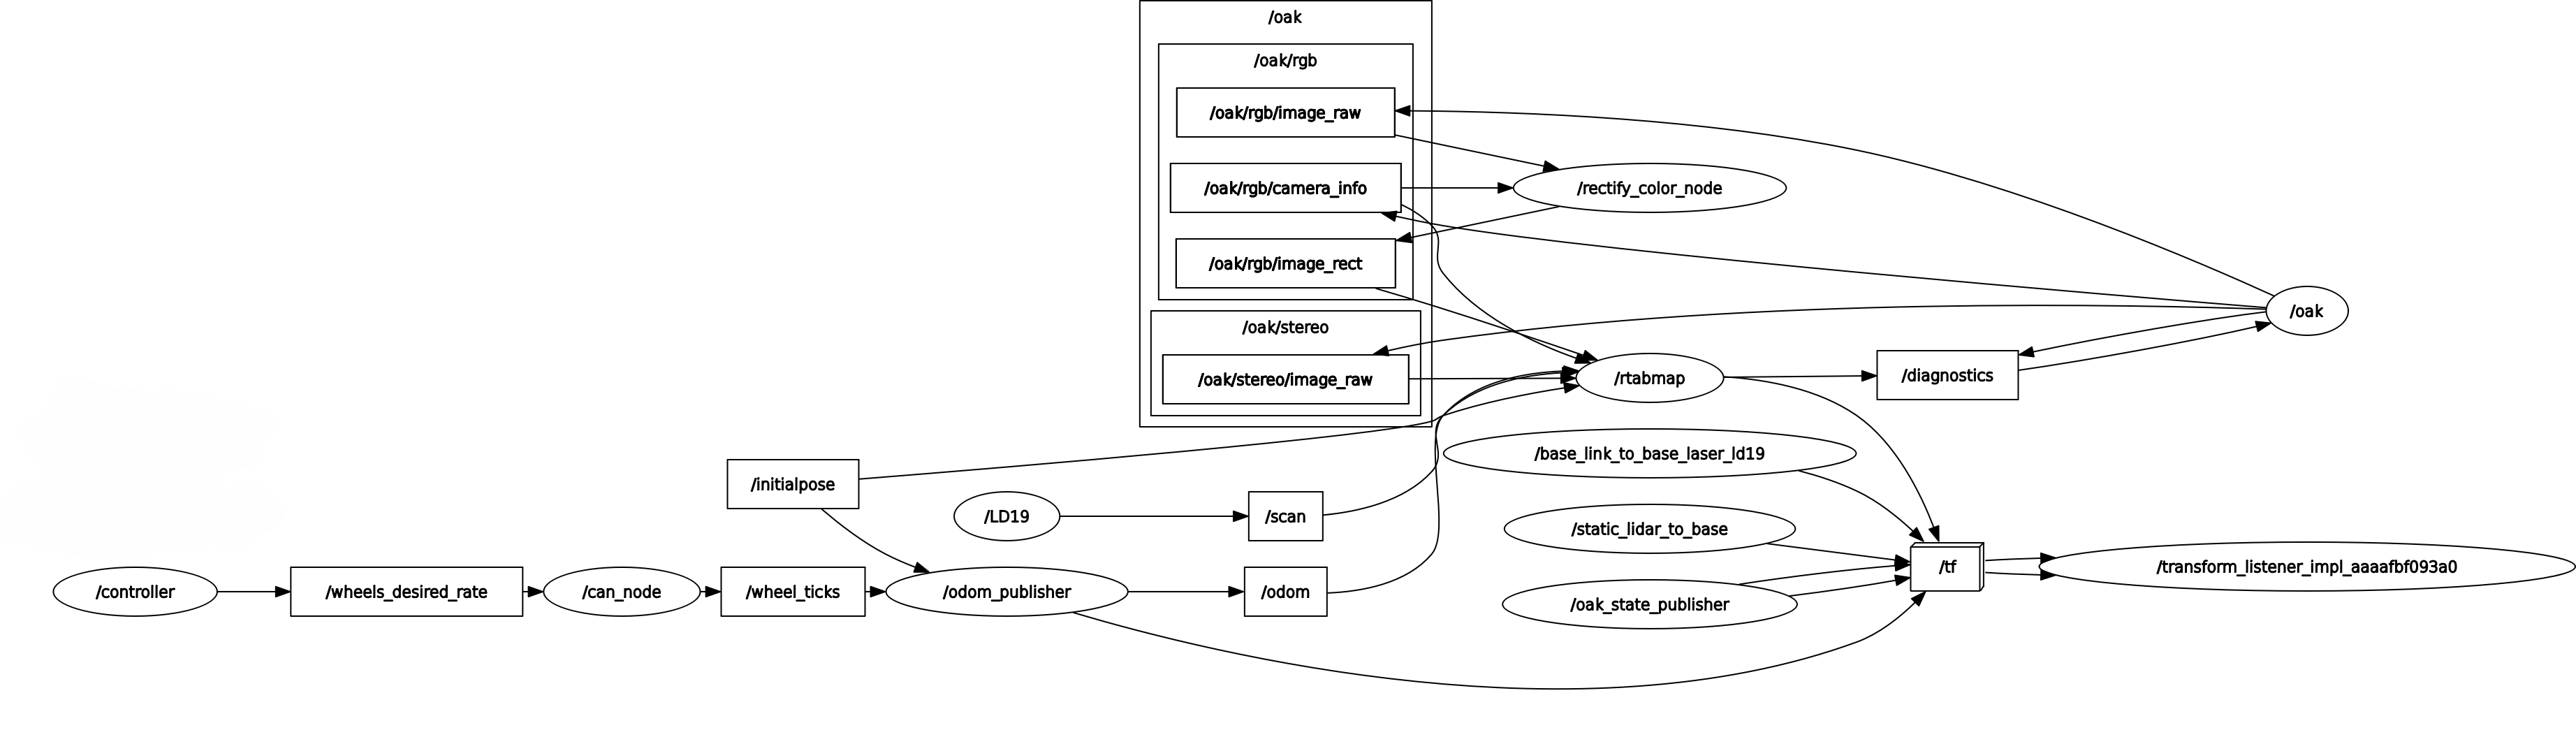
\includegraphics[width=1\textwidth]{imgs/rosgraph.png}
  \caption{ROS 2 node graph}
  \label{fig:ros2_node_graph}
\end{figure}

\begin{figure}[H]
  \centering
  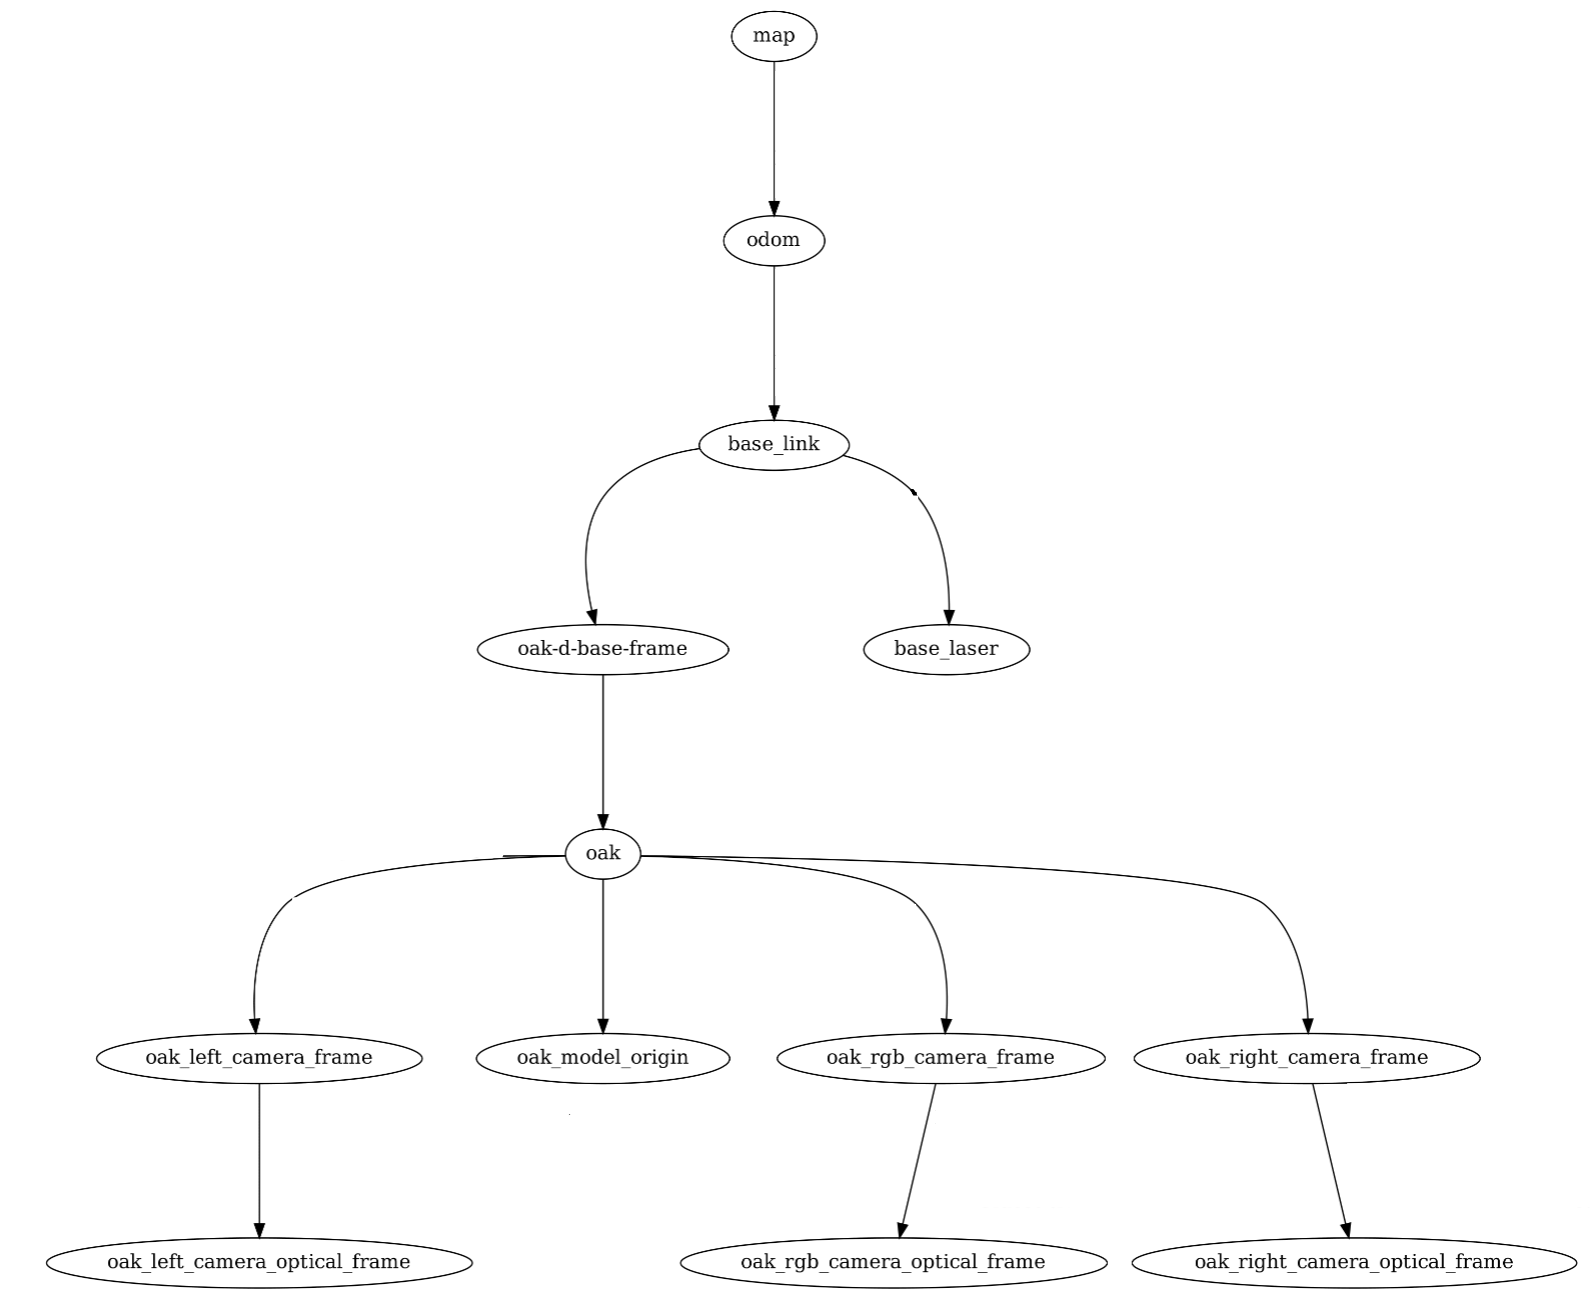
\includegraphics[width=0.8\textwidth]{imgs/frames_2025-05-30_13.29.21-1.png}
  \caption{ROS 2 TF tree}
  \label{fig:ros2_tf_tree}
\end{figure}
% ------------------------------------------------------------------------------
% Implementation and Experimental Results Chapter
% ------------------------------------------------------------------------------

% NOTE: Replace the file names in \includegraphics with the actual image files
% you will add to the `imgs/` folder. Each sub-figure has its own label for
% cross-referencing if needed.

% ==============================================================================
\chapter{Implementation \& experimental results}\label{ch:implementation}

% ------------------------------------------------------------------------
\section{Experimental setup}
\label{sec:exp_setup}

\paragraph*{Test arenas}
\label{sec:test_arenas}

All trials were carried out in two controlled indoor environments:

\begin{enumerate}[label=(\alph*)]
  \item \textbf{Laboratory \texttt{l009} (ESIDE Building).}
        A room with a smooth tile floor that introduces low friction and wheel slippage for the robot's mecanum wheels, well illuminated and Removable furniture (tables, chairs) acts simultaneously as navigation hazards and visual features, facilitating loop-closure opportunities for the algorithms, Nevertheless, confusing it in the \gls{bovw} due the high similarity between them.

  \item \textbf{Basement Corridor (ESIDE Building).}
        A corridor characterized by low ambient illumination and painted walls that challenges the feature matching algorithm.
\end{enumerate}


\paragraph*{Ground truth acquisition}
\label{sec:gt_acquisition}

In the absence of an optical motion capture instruments, ground truth was approximated by manually observing the robot's trajectory and the map it generated. The robot was driven autonomously in both arenas by automating the sending of navigation commands to near points in the costmap, while the \gls{rtab} node was recording the robot's trajectory and the map it generated. The robot's position was recorded at each point in the map.

\section{Results}
\label{sec:results}

The experimental results are presented in Figure~\ref{fig:results} where the path of the robot is shown in blue, because of the complexity of the 3D maps, only representative views are presented here. A set of 3D reconstructions and 2D images comparison is available in the appendix~\ref{app:extended_results}.

\begin{figure}[H]
  \centering
  \begin{subfigure}[b]{0.45\textwidth}
    \centering
    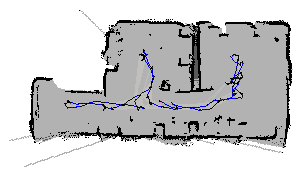
\includegraphics[width=\textwidth]{imgs/gridlab.png}
    \caption{Laboratory \texttt{l009} grid map}
    \label{fig:results_lab2d}
  \end{subfigure}
  \begin{subfigure}[b]{0.45\textwidth}
    \centering
    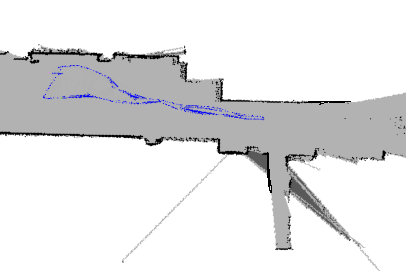
\includegraphics[width=\textwidth]{imgs/gridcorri.png}
    \caption{Basement corridor grid map}
    \label{fig:results_corridor2d}
  \end{subfigure}
  \begin{subfigure}[b]{0.49\textwidth}
    \centering
    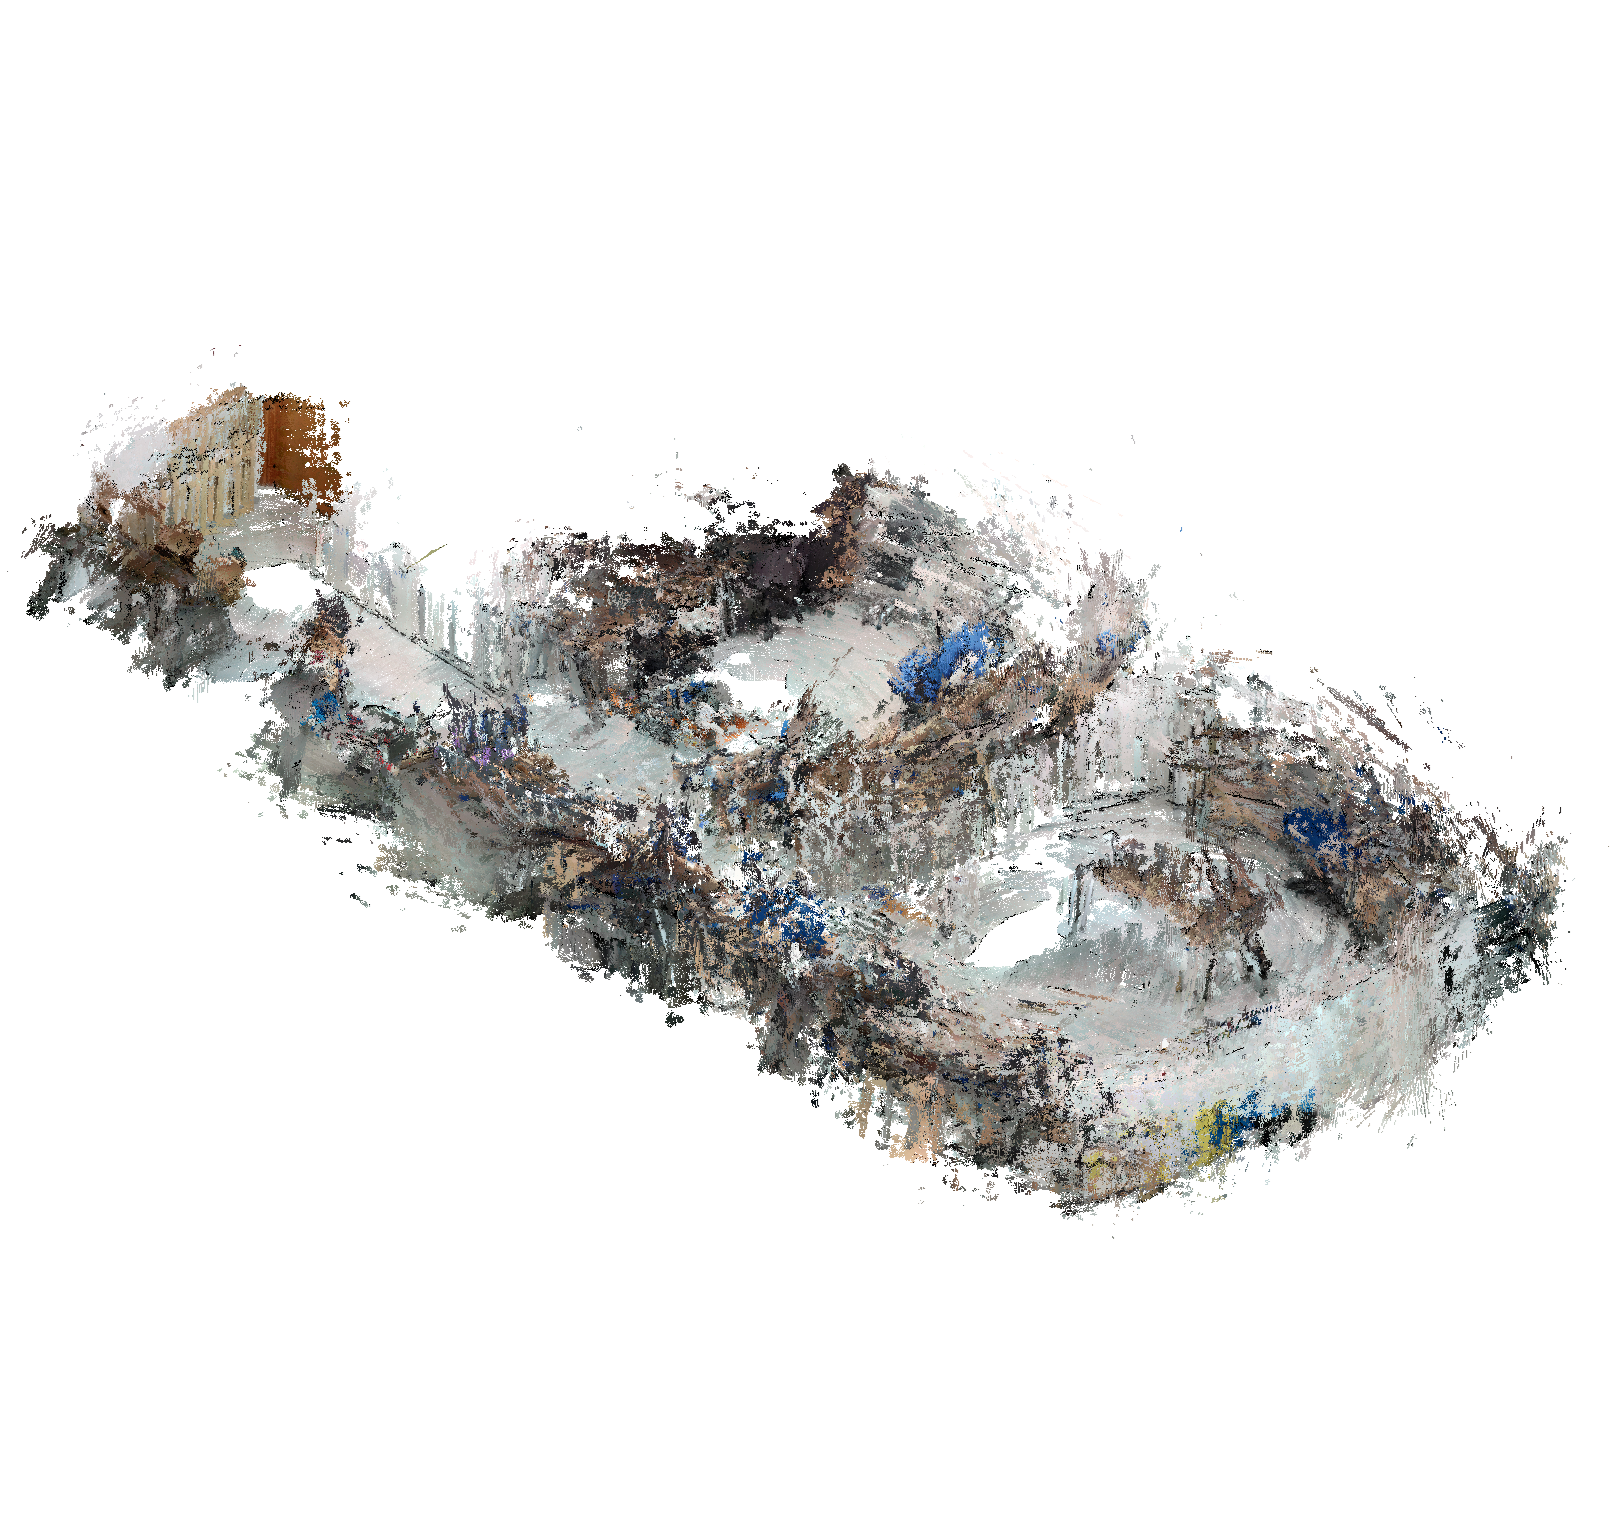
\includegraphics[width=\textwidth]{imgs/isolab.png}
    \caption{Laboratory \texttt{l009} 3D map}
    \label{fig:results_lab3d}
  \end{subfigure}
  \begin{subfigure}[b]{0.49\textwidth}
    \centering
    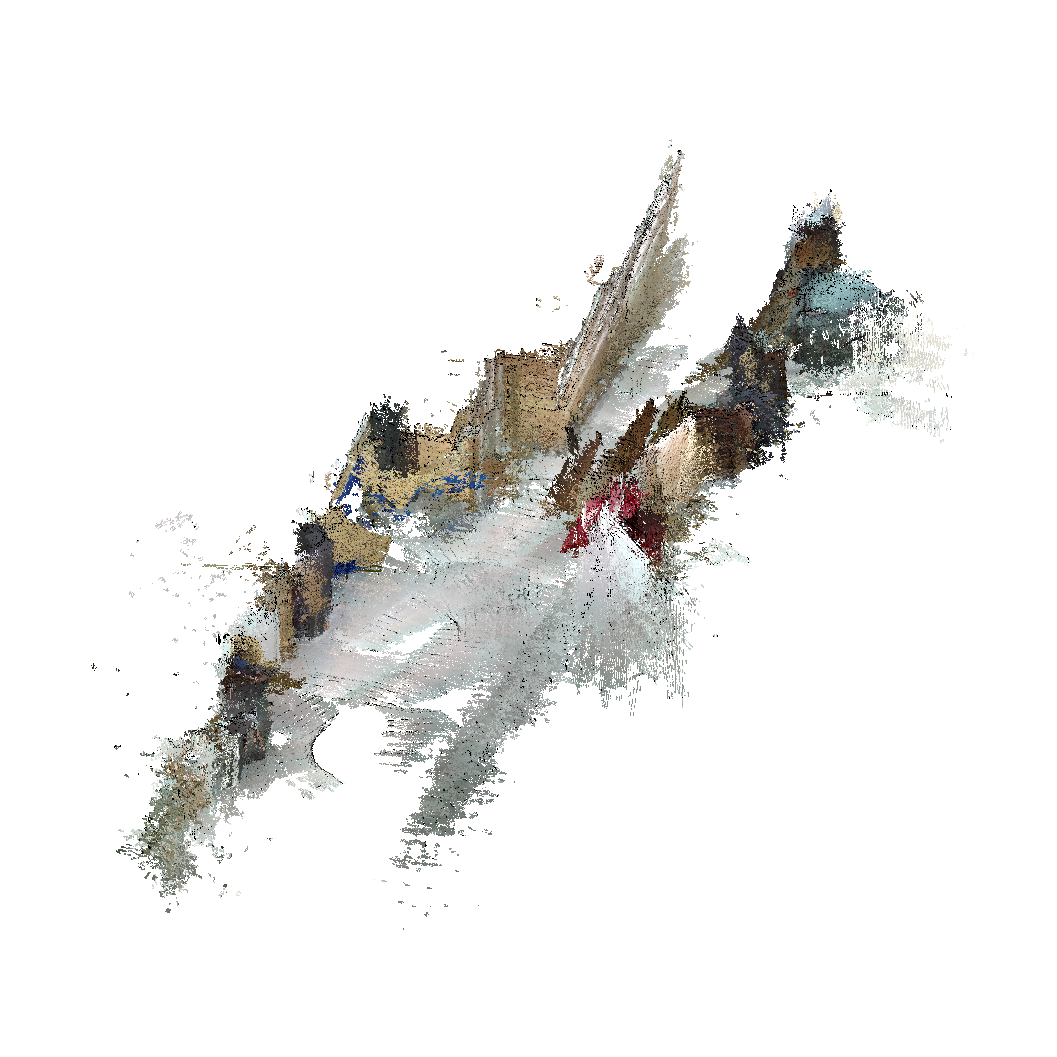
\includegraphics[width=\textwidth]{imgs/isocorri.png}
    \caption{Basement Corridor 3D map}
    \label{fig:results_corridor3d}
  \end{subfigure}
  \caption{Experimental results}
  \label{fig:results}
\end{figure}



\section{Discussion}
\label{sec:discussion}

The robot was able to navigate autonomously in both arenas, generating both the 2D and 3D maps. As for the 2D maps, the robot was able to generate both maps with a good accuracy, as the \gls{lidar} is independent from ambient conditions, the difference between real dimensions and the generated map is less than \SI{2.4}{\percent} when measured in different locations in the map. This difference is due to odometry drift and the \gls{lidar} noise, which is expected in such a system.\\
The 3D maps generated by the robot where noisy and lack features when matching the RGB with the depth, making them less useful without prior knowledge of the environment. These problems come from the fact that the \textbf{Oak-D lite} camera processes the depth calculations internally, which after reviewing the data, it was found that the depth information was not accurate enough for reliable 3D mapping. Also, doing the calculations internally reduced the frame rate significantly to around \SI{3}{\hertz}, which is not enough for a reliable 3D mapping.
Nevertheless, after some noise reduction and filtering, a 3D grid map was generated, which can be seen in Figure~\ref{fig:3dgridresaults}, these two maps have acceptable accuracy but not enough features to be used for navigation.\\
Regarding the autonomous navigation, the robot was able to navigate autonomously in both arenas when commanded to a setpoints in the costmap with a difference of less than \SI{7}{\centi\meter} from the center of the base, this difference is due to the limited ability to control the motors at low speeds (minimum speed is \SI[per-mode=fraction,fraction-function=\tfrac]{0.1}{\metre\per\second}), which is not enough for precise navigation.

\begin{figure}[H]
  \centering
  \begin{subfigure}[b]{0.45\textwidth}
    \centering
    
\includegraphics[width=\textwidth]{imgs/3dgridlab.png}
    \caption{Laboratory \texttt{l009} 3D grid map}
    \label{fig:results_3dlabg}
  \end{subfigure}
  \begin{subfigure}[b]{0.45\textwidth}
    \centering
    
\includegraphics[width=\textwidth]{imgs/3d grid.png}
    \caption{Basement corridor 3D grid map}
    \label{fig:3dgridcorri}
  \end{subfigure}
  \caption{3D grid maps}
  \label{fig:3dgridresaults}
\end{figure}
% ------------------------------------------------------------------------
\section{Power analysis}
\label{sec:power_analysis}

Let the average supply voltage of a converter or the battery be \(V_{src}\) and the battery's nominal capacity is $C=$\SI{10}{\ampere\hour}.
For each electrical subsystem, the measured steady state current is \(I_{sys}\) and the duty cycle weighted utilization factor by \(\gamma_{sys}\in[0,1]\).
The instantaneous power and total energy consumption are

\begin{equation}
  P_{sys} = V_{src}\,I_{sys}\,\gamma_{sys},
  \qquad
  P_{\mathrm{tot}} = \sum_{sys} P_{sys},
  \qquad
  E_{\mathrm{tot}} = P_{\mathrm{tot}}\,t,
  \label{eq:power}
\end{equation}

where \(t\) is the operating time.
Solving \eqref{eq:power} for \(t\) yields the theoretical autonomy

\begin{equation}
  t_{\max} = \frac{V_{bat}\,C\,\eta_\mathrm{bat}}{\sum_{sys} V_{src}\,I_{sys}\,\gamma_{sys}}
  \label{eq:runtime}
\end{equation}

with \(\eta_\mathrm{bat}\approx0.9\) accounting for Peukert losses and DC-DC conversion inefficiencies.

\begin{table}[H]
  \centering
  \label{tab:power_budget}
  \begin{tabular}{l c c c}
    \toprule
    \textbf{Subsystem}
     & \textbf{Current}~$I_{sys}$~[A]
     & \textbf{Duty}~$\gamma_{sys}$
     & \textbf{Power}~$P_{sys}$~[W]   \\
    \midrule
    MCU
     & $0.15$
     & $1$
     & $0.5$                          \\

    Jetson Orin Nano
     & $1.3$
     & $1$
     & $15.6$                         \\

    Motors
     & $1.5$
     & $0.5$
     & $16.8$                         \\
    Modules
     & $0.6$
     & $1$
     & $3$                            \\
    \midrule
    \textbf{Total}
     &
     &
     & $35.9$                         \\
    \bottomrule
  \end{tabular}
  \caption{Components power budget}
\end{table}



Under typical indoor workloads, preliminary bench tests suggest a mapping runtime in the \SIrange{5}{6}{\hour} range.
% ------------------------------------------------------------------------




\chapter{Future work}\label{ch:future_work}

The current implementation of the robot is a proof-of-concept that demonstrates the functionality of the \gls{slam} algorithm, however, there are several areas for improvement and future work that can be explored.

\section{Hardware improvements}

\begin{itemize}
  \item \textbf{IMU integration}: As seen in the results, the robot's odometry has margin of improvement, this can be achieved by integrating an \gls{imu} sensor to provide additional information about the robot's orientation and acceleration, which can help to improve the accuracy of the odometry.
  \item \textbf{\gls{ir} sensor integration}: Adding an \gls{ir} sensor helps with aligning the RGB and depth images, improving the system's ability to generate accurate 3D maps, reducing the dependencies on the stereo calculations the showed limitations as seen in the results.
  \item \textbf{Custom PCB}: The current implementation uses modules that are connected via cables, which lack cable management and can be prone to disconnections and accidental short circuit. A custom \gls{pcb} can be designed to integrate all the modules and sensors, providing a more robust and reliable solution.
\end{itemize}
\section{Software improvements}
\begin{itemize}
  \item \textbf{EKF integration}: Fusing the odometry data with the \gls{imu} data using an \gls{ekf} can significantly improve the accuracy of the robot's pose estimation. The \gls{ekf} can combine the noisy odometry data with the more reliable \gls{imu} data to produce a more accurate estimate of the robot's position and orientation.
  \item \textbf{Stereo depth processing}: Moving the Stereo depth processing to the main computer can help with the depth calculations, Nevertheless, better results are not guaranteed.
  \item \textbf{loop closure detection}: Adding a post processing step to the \gls{slam} algorithm that detects loop-closures can help with the time-of-flight implementation, achieving more processed frames per second, and improving the overall accuracy of the 3D map.
  \item \textbf{Lower level optimizations}: The current Code for the \gls{ros}~2 nodes is written in Python, which is not the most efficient language for time-of-flight processing. Rewriting the code in C++ can significantly improve the performance of the nodes.
  \item \textbf{ROS~2 containerization}: The node run on different processes and the communication between them is done via \gls{ros}~2 topics, however, this can be improved by using \gls{ros}~2 containers to run nodes in a single process, which can reduce the overhead of inter process communication and improve the overall performance of the system~\footnote{Only the containerization of the camera, \gls{lidar} and odometry nodes is considered, because the containerization of the other nodes can stop all processes if any fails.}.
\end{itemize}

\chapter{Ethical considerations}\label{ch:ethics}

Ethical considerations in robotics are not less important than in other engineering concerns. It must be clear since the beginning whether the robot serves its intended beneficial purpose without introducing harms, and that private interest is balanced with public good. The IEEE's \textit{Ethically Aligned Design}~\cite{8058187} says that \say{We need to make sure that these technologies are aligned to humans in terms of our moral values and ethical principles. autonomous systems have to behave in a way that is beneficial to people beyond reaching functional goals and addressing technical problems}.\\
With the acceleration of robotics, labor and social justice issues arise, as robots are increasingly replacing human workers in various industries. Nevertheless, from the perspective many workers, it is seen as a benefit for their safety and comfort at work, their pay, and their autonomy on the job~\cite{armstrong2024automationworkersperspective}.\\
The intention of this project is not to create a robot that replaces human workers, but rather to create a robot that can assist humans in their work, and make it safer. In the last years, the use of robots in hazardous environments has increased, from the 2010 haiti earthquake to the Deepwater Horizon oil spill where it helped in the search and rescue operations~\cite{10.7551/mitpress/9407.003.0012}.\\
Professional responsibility adds to the idea, every engineer shares legal obligation and moral responsibility to Incorporate professional ethics into their work such as social justice, environmental sustainability, and human rights. The project combines a deontological stance with utilitarian view, establishing duties, while optimizing for measurable benefits such as lower injuries and broader workplace inclusion.\\
In sum, autonomous robots provide an extraordinary opportunity yo improve the quality of life and work, To ensure that they uplift rather than burden the human condition, a human-centered approach is essential. This includes continuous upskilling and reconversion programs for affected workers and democratized access to technical training. Industry standards such as ISO 13482 and ISO/TS 15066 provide concrete guidance for safe, inclusive design, but must be augmented by social assessments and community engagement.
The present work can be assessed with the four engineering ethical concepts: beneficence, non-maleficence, autonomy and justice. Beneficence is addressed with what is mentioned previously, helping with the well-being of humans.
Non-maleficence is satisfied through the implementation of emergency stops, low maximum speed, battery an voltage management, all of which lower the probability accidental hazards.
Respect for autonomy is preserved by publishing the software stack, users retain the ability to inspect and audit robot behavior.
Justice is promoted by keeping the bill of materials below 1500 \euro so that smaller institutions can adopt the technology.


\chapter{Work plan \& budget}\label{sec:work_plan_budget}

\section{Work plan \& Gantt diagram}

The project started on \textbf{28~February~2025} and is scheduled for completion on \textbf{15~June~2025}. Table~\ref{tab:phases} summarizes each phase, its principal deliverable and the nominal duration.

\begin{table}[H]
  \centering
  \begin{tabular}{llc}
    \toprule
    \textbf{Phase}        & \textbf{Deliverable}         & \textbf{Duration (weeks)} \\
    \midrule
    Design of robot       & Preliminary CAD              & 2                         \\
    Component selection   & Bill of materials            & 2                         \\
    Programming of MCU    & Embedded firmware repository & 4                         \\
    Programming of ROS~2  & ROS~2 workspace              & 4                         \\
    Testing               & Validation report            & 2                         \\
    Elaboration of memory & Final dissertation           & 11                        \\
    \bottomrule
  \end{tabular}
  \caption{Phases, deliverables and duration}
  \label{tab:phases}
\end{table}


\begin{sidewaysfigure}
  \centering
  \begin{ganttchart}[
      hgrid,
      vgrid,
      time slot format=isodate,
      x unit=0.14cm,                   % Squeeze horizontally
      y unit chart=1.3cm,              % Squeeze vertically
      title height=1.2,                % Reduce title row height
      title label font=\scriptsize\bfseries,
      bar/.append style={fill=black!30},
      bar label font=\bfseries,   % Smaller bar labels
      milestone label font=\bfseries,
      bar height=0.4,                  % Thinner bars
      group height=0.5,
    ]{2025-02-15}{2025-06-20}
    \gantttitlecalendar{month=shortname}\\
    \ganttbar{Design of robot}{2025-02-28}{2025-03-14}\\
    \ganttbar{Component selection}{2025-03-15}{2025-03-28}\\
    \ganttbar{Programming of MCU}{2025-03-29}{2025-04-25}\\
    \ganttbar{Programming of ROS2}{2025-04-26}{2025-05-23}\\
    \ganttbar{Testing}{2025-05-24}{2025-06-08}\\
    \ganttbar{Elaboration of memory}{2025-04-01}{2025-06-15}\\
    \ganttmilestone{Submission}{2025-06-15}
  \end{ganttchart}
  \caption{Project Gantt chart}
  \label{fig:gantt}
\end{sidewaysfigure}

\section{Budget}

In accordance with regulations and guidelines, the budget has been estimated considering the hourly cost of the student (15\euro) and the supervisor (50\euro). The breakdown is shown in Table~\ref{tab:costs}.

\begin{table}[H]
  \centering
  \begin{tabular}{l
      S[table-format=3.0]
      S[table-format=3.0]
      S[table-format=5.0]}
    \toprule
    \textbf{Activity}     & {\textbf{Student hours}} & {\textbf{Supervisor hours}} & {\textbf{Total cost (\euro)}} \\
    \midrule
    Design of robot       & 20                       & 3                           & 450                           \\
    Component selection   & 29                       & 2                           & 535                           \\
    Programming of MCU    & 77                       & 3                           & 1305                          \\
    Programming of ROS~2  & 147                      & 4                           & 2405                          \\
    Testing               & 15                       & 0                           & 225                           \\
    Elaboration of memory & 50                       & 3                           & 900                           \\
    \midrule
    \textbf{Totals}       & 338                      & 15                          & 5820                          \\
    \bottomrule
  \end{tabular}
  \caption{Estimated project costs}
  \label{tab:costs}
\end{table}

the costs of the components used in the project are summarized in Table~\ref{tab:bom}. The total cost of the components is 1175\euro.

\begin{table}[H]
  \centering
  \sisetup{round-mode=places, round-precision=0}
  \begin{tabular}{l
      S[table-format=3.0]
      S[table-format=5.0]}
    \toprule
    \textbf{Component} & {\textbf{Qty.}} & {\textbf{Cost (\euro)}} \\
    \midrule
    Jetson Orin Nano   & 1               & 250                     \\
    MCU                & 1               & 12                      \\
    Motor drivers      & 2               & 134                     \\
    CAN module         & 1               & 3                       \\
    Li-ion battery     & 1               & 170                     \\
    DC-DC converter    & 3               & 33                      \\
    BMS                & 1               & 39                      \\
    Camera             & 1               & 149                     \\
    LiDAR              & 1               & 66                      \\
    Motors             & 4               & 96                      \\
    Wheels             & 4               & 187                     \\
    Chassis            &                 & 24                      \\
    Misc. wiring       &                 & 12                      \\
    \midrule
    \textbf{Totals}    &                 & 1175                    \\
    \bottomrule
  \end{tabular}
  \caption{Bill of materials}
  \label{tab:bom}
\end{table}

The total project cost is 6995\euro, reflecting both the student's effort, the supervisory guidance provided throughout the development lifecycle and the costs of the components used in the project.

%% ----------------------
%% Bibliografía y apéndices
%% ----------------------


\backmatter

\bibliografia{referencias}



\chapter*{Acknowledgment}\addcontentsline{toc}{chapter}{Acknowledgment}

Deepest gratitude is extended to PhD. Javier Vicente Sáez, project director, for invaluable guidance and unwavering support throughout this work. Generous provision of all required materials facilitated experimental work, and unrestricted access to Laboratory L009 ensured successful completion of the project.

\printglossary[type=main, title=Glossary]\addcontentsline{toc}{chapter}{Glossary}
\printglossary[type=acronym, title=Acronyms]\addcontentsline{toc}{chapter}{Acronyms}

\appendix

\chapter{User manual}\label{appendix:user_manual}

This user manual describes the steps required to build, flash, and operate the mobile robot platform. It covers firmware tooling, \gls{ros}~2 workspace setup, and operating system configuration.

\section{MCU firmware: build \& flash workflow}

\subsection{Prerequisites}
Ensure the following components are installed on Ubuntu 22.04 or equivalent:
\begin{itemize}
\item GNU Arm Embedded Toolchain v12.3-Rel1 or newer
\item CMake $\geq$ 3.25
\item OpenOCD 0.12.0 \emph{or} STM32CubeProgrammer 2.15
\item \texttt{stlink-tools} 1.7 (optional, for \texttt{st-flash})
\end{itemize}
Install via:
\begin{lstlisting}[language=bash]
sudo apt update
sudo apt install gcc-arm-none-eabi cmake make openocd stlink-tools
\end{lstlisting}

\subsection{Building the firmware}
\begin{enumerate}
\item Change into the firmware directory:
\begin{lstlisting}[language=bash]
cd MCU
\end{lstlisting}
\item Configure the build:
\begin{lstlisting}[language=bash]
cmake -B build -DCMAKE\_BUILD\_TYPE=Release
\end{lstlisting}
\item Compile:
\begin{lstlisting}[language=bash]
cmake --build build -j\$(nproc)
\end{lstlisting}
\item The outputs (\texttt{plub\_plub.elf}, \texttt{plub\_plub.bin}) will be in \texttt{MCU/build/}.
\end{enumerate}

\subsection{Flashing the firmware}
\paragraph*{Option A: OpenOCD}
\begin{lstlisting}[language=bash]
openocd -f interface/stlink.cfg
openocd -f target/stm32f4x.cfg
openocd -c "program build/plub\_plub.elf verify reset exit"
\end{lstlisting}

\paragraph*{Option B: ST-LINK CLI}
\begin{lstlisting}[language=bash]
st-flash write build/plub\_plub.bin 0x08000000
\end{lstlisting}

\noindent Verify successful programming:
\begin{lstlisting}[language=bash]
openocd -f interface/stlink.cfg
openocd -f target/stm32f4x.cfg
openocd -c "mdw 0x08000000 4"
\end{lstlisting}

\section{ROS 2 workspace setup}

\subsection{System dependencies}
Install \gls{ros}~2 Humble and related packages:
\begin{lstlisting}[language=bash]
sudo apt install ros-humble-desktop
sudo apt install python3-colcon-common-extensions
sudo apt install ros-humble-ros2-control
sudo apt install ros-humble-ros2-controllers
sudo apt install ros-humble-rosbridge-suite
sudo apt install can-utils
\end{lstlisting}

\subsection{Building the workspace}
\begin{enumerate}
\item Enter the workspace:
\begin{lstlisting}[language=bash]
cd plub\_plub\_ws
\end{lstlisting}
\item Install dependencies:
\begin{lstlisting}[language=bash]
rosdep install --from-paths src --ignore-src -y
\end{lstlisting}
\item Build:
\begin{lstlisting}[language=bash]
colcon build --symlink-install
\end{lstlisting}
\item Source:
\begin{lstlisting}[language=bash]
source ./install/setup.bash
\end{lstlisting}
\end{enumerate}

\subsection{Launching the full stack}
\begin{lstlisting}[language=bash]
ros2 launch run run.launch.py
\end{lstlisting}

\section{Operating system configuration}

\subsection{Serial \& USB permissions}
Grant access to the USB serial port:
\begin{lstlisting}[language=bash]
sudo chmod 777 /dev/ttyUSB0
lsusb \
  | awk '/03e7/ { gsub(/:$/,"",$4); printf "/dev/bus/usb/%03d/%03d\n", $2, $4 }' \
  | xargs sudo chmod 666
\end{lstlisting}

\subsection{CAN channel initialization}
\begin{lstlisting}[language=bash]
sudo ip link set can1 type can bitrate 500000
sudo ip link set can1 up
candump can1
\end{lstlisting}

\chapter{Comprehensive parameter listing}\label{app:launch_params}

To ensure full experimental reproducibility, this appendix exhaustively
enumerates the runtime parameters that are injected into each \gls{ros}~2 node at
launch. Unless otherwise stated, the values correspond to those employed
throughout the evaluation campaign presented in Chapter~\ref{ch:implementation}. Boolean parameters are listed as \texttt{true}/\texttt{false};
hexadecimal integers are formatted with a \texttt{0x}~prefix.

%-------------------------------------------------------------------------------
\section{\texttt{can\_communication} package}
\subsection{\texttt{can\_node}}
\begin{longtable}{@{}llp{0.60\textwidth}@{}}
  \toprule
  \textbf{Parameter} & \textbf{Type} & \textbf{Description} \\
  \midrule
  \endhead
  can\_interface      & string & Host \gls{can} interface bound to the socket. \\[-4pt]
  tx\_can\_id          & uint32 & Arbitration ID used for outgoing frames. \\[-4pt]
  rx\_can\_id          & uint32 & Hardware filter mask for incoming frames. \\[-4pt]
  bitrate             & uint32 & Bus bitrate in \nicefrac{bits}{sec}. \\[-4pt]
  filter\_incoming     & bool   & Enables kernel level RX filtering. \\
  \bottomrule
\end{longtable}

\section{\texttt{ldlidar\_ros2} package}
\subsection{\texttt{ldlidar\_ros2\_node}}
\begin{longtable}{@{}llp{0.60\textwidth}@{}}
  \toprule
  \textbf{Parameter} & \textbf{Type} & \textbf{Description} \\
  \midrule
  product\_name            & string & LiDAR model identifier. \\[-4pt]
  topic\_name              & string & Topic onto which the \texttt{sensor\_msgs/LaserScan} is published. \\[-4pt]
  frame\_id                & string & Reference frame attached to the LiDAR optical centre. \\[-4pt]
  port\_name               & string & Serial device path of the bridge. \\[-4pt]
  laser\_scan\_dir         & bool   & \texttt{true}: counter/clockwise; \texttt{false}: clockwise scan order. \\[-4pt]
  enable\_angle\_crop\_func & bool   & Activates angular masking of the raw scan. \\[-4pt]
  angle\_crop\_min         & float  & Inclusive lower bound of the angular mask (\si{\degree}). \\[-4pt]
  angle\_crop\_max         & float  & Inclusive upper bound of the angular mask (\si{\degree}). \\
  \bottomrule
\end{longtable}

\section{\texttt{mecanum\_drive} package}\label{app:mecanum_drive_params}

\subsection{\texttt{mecanum\_drive\_controller}}

\begin{longtable}{@{}lll@{}}
\toprule
\textbf{Parameter} & \textbf{Value} & \textbf{Description} \\
\midrule
ticks\_per\_meter          & 4332.0 & Encoder ticks that correspond to one metre of tangential wheel travel. \\
wheel\_separation          & 0.34   & Lateral distance between the mid points of the left and right wheel contact patches (m). \\
wheel\_separation\_length  & 0.24   & Longitudinal distance between the front and rear axle lines (m). \\
max\_motor\_speed          & 3456   & Upper bound on the actuator command (\nicefrac{ticks}{second}). \\
\bottomrule
\end{longtable}

\subsection{\texttt{mecanum\_drive\_odometry}}

\begin{longtable}{@{}lll@{}}
\toprule
\textbf{Parameter} & \textbf{Value} & \textbf{Description} \\
\midrule
ticks\_per\_meter          & 4332.0 & Same conversion factor as for the controller, ensuring kinematic coherence. \\
wheel\_separation          & 0.34   & Lateral baseline (m). \\
wheel\_separation\_length  & 0.24   & Longitudinal baseline (m). \\
base\_frame\_id            & \texttt{base\_link} & Name of the robot's body frame in the \textsf{tf2} tree. \\
odom\_frame\_id            & \texttt{odom}       & Fixed world frame used for integrating wheel displacements. \\
encoder\_min               & $-32\,768$ & Lower bound of the 16-bit encoder counter. \\
encoder\_max               & $32\,767$  & Upper bound of the 16-bit encoder counter. \\
\bottomrule
\end{longtable}

\section{\texttt{depthai\_ros\_driver} package}
The OAK-D camera driver is launched via the vendor/supplied
\texttt{camera.launch.py}. The only top/level parameters injected by
\texttt{global.launch.py} are the camera namespace (name) and the
path to an external YAML file (params\_file). The contents of that
YAML are vendor maintained and excluded here for brevity.

\section{\texttt{rtabmap\_slam} package}

\begin{longtable}{@{}llp{0.60\textwidth}@{}}
  \toprule
  \textbf{Parameter} & \textbf{Value} & \textbf{Description} \\
  \midrule
  \endhead
  frame\_id                      & \texttt{base\_link}  & align data with the vehicle frame. \\[-4pt]
  subscribe\_rgb                 & \texttt{true}        & enable RGB stream subscription. \\[-4pt]
  subscribe\_depth               & \texttt{true}        & enable aligned depth stream subscription. \\[-4pt]
  subscribe\_scan                & \texttt{true}        & fuse 2D LiDAR scan into occupancy grid. \\[-4pt]
  subscribe\_odom\_info          & \texttt{false}       & disable odometry info subscription. \\[-4pt]
  subscribe\_imu                 & \texttt{false}       & disable IMU data subscription. \\[-4pt]
  sync\_queue\_size              & \texttt{10}          & bound message filter queue length. \\[-4pt]
  approx\_sync                   & \texttt{true}        & enforce approximate time synchronization heuristic. \\[-4pt]
  approx\_sync\_max\_interval    & \SI{0.001}{s}        & maximum allowed timestamp difference for sync. \\[-4pt]
  visual\_odometry               & \texttt{false}       & disable visual odometry feature. \\[-4pt]
  delete\_db\_on\_start          & \texttt{true}        & clear the database at startup. \\[-4pt]
  FAST/gpu                       & \texttt{true}        & enable GPU acceleration for FAST feature detection. \\[-4pt]
  Grid/Sensor                    & \texttt{0}           & sensor ID to use for occupancy grid integration (LiDAR). \\[-4pt]
  RGBD/NeighborLinkRefining      & \texttt{true}        & refine graph links between spatially close nodes. \\[-4pt]
  RGBD/ProximityBySpace          & \texttt{true}        & create links based on spatial proximity. \\[-4pt]
  RGBD/AngularUpdate             & \num{0.05}           & angular threshold (rad) for creating a new keyframe. \\[-4pt]
  RGBD/LinearUpdate              & \num{0.05}           & linear threshold (m) for creating a new keyframe. \\[-4pt]
  Grid/RangeMax                  & \SI{11.5}{m}         & clip occupancy grid integration beyond this radius. \\[-4pt]
  Grid/RangeMin                  & \SI{0.5}{m}          & ignore depth measurements closer than this radius. \\[-4pt]
  Grid/FromDepth                 & \texttt{false}       & disable building grid directly from depth images. \\[-4pt]
  Reg/Force3DoF                  & \texttt{true}        & constrain on odometry ($x,y,\theta$). \\[-4pt]
  Reg/Strategy                   & \texttt{1}           & registration strategy selector. \\[-4pt]
  RGBD/ProximityByTime           & \texttt{false}       & disable linking based on temporal proximity. \\[-4pt]
  RGBD/ProximityPathMaxNeighbors & \texttt{10}          & max neighbors to consider in proximity path search. \\[-4pt]
  RGBD/LocalRadius               & \num{5}              & radius (m) for local link detection. \\[-4pt]
  Vis/MinInliers                 & \texttt{10}          & minimum inliers required for visual registration. \\[-4pt]
  RGBD/OptimizeFromGraphEnd      & \texttt{false}       & disable incremental optimization from graph end. \\[-4pt]
  RGBD/OptimizeMaxError          & \texttt{4}           & maximum allowed error for graph optimization. \\[-4pt]
  Icp/CorrespondenceRatio        & \num{0.2}            & ratio of correspondences to keep during ICP. \\[-4pt]
  Icp/PM                         & \texttt{false}       & disable point-to-mesh correspondence. \\[-4pt]
  Icp/PointToPlane               & \texttt{false}       & disable point-to-plane ICP mode. \\[-4pt]
  Icp/MaxCorrespondenceDistance  & \SI{0.1}{m}          & tighter point-plane ICP constraint. \\[-4pt]
  Icp/VoxelSize                  & \SI{0.05}{m}         & down/up-sample point clouds for ICP. \\
  \bottomrule
\end{longtable}


The remaining parameters retain their package
defaults and are therefore omitted.

\chapter{extended results}\label{app:extended_results}

This appendix provides additional results that were not included in the main body of the thesis. The data presented here is intended to support the findings and conclusions drawn in the results chapter.
A photo of the 3D reconstructions and scene from robot perspective is shown in each figure.

\begin{figure}[H]
  \centering
  \begin{subfigure}[b]{0.47\textwidth}
    \centering
    \includegraphics[height=6cm,width=\textwidth]{imgs/lc1.png}
    \caption{Point cloud}

  \end{subfigure}
  \hfill
  \begin{subfigure}[b]{0.47\textwidth}
    \centering
    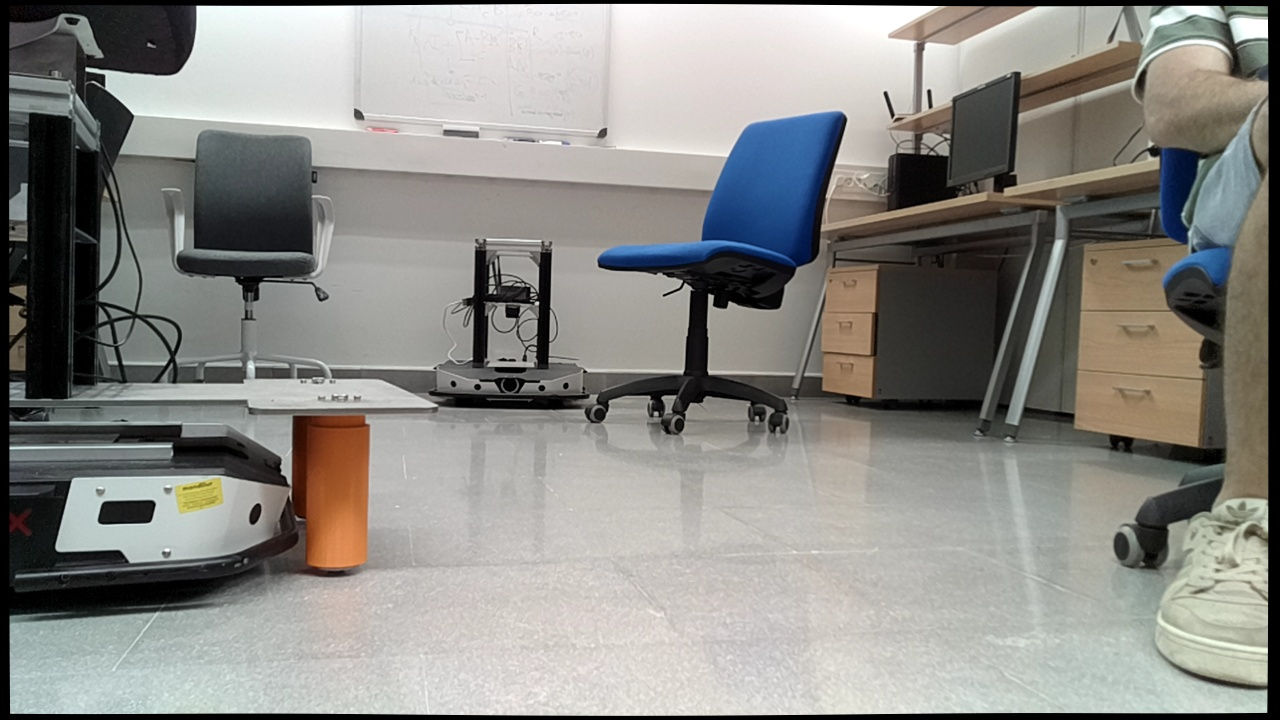
\includegraphics[height=6cm,width=\textwidth]{imgs/lr1.png}
    \caption{RGB}

  \end{subfigure}
\end{figure}

\begin{figure}[H]
  \centering
  \begin{subfigure}[b]{0.47\textwidth}
    \centering
    \includegraphics[height=6cm,width=\textwidth]{imgs/lc3.png}
    \caption{Point cloud}

  \end{subfigure}
  \hfill
  \begin{subfigure}[b]{0.47\textwidth}
    \centering
    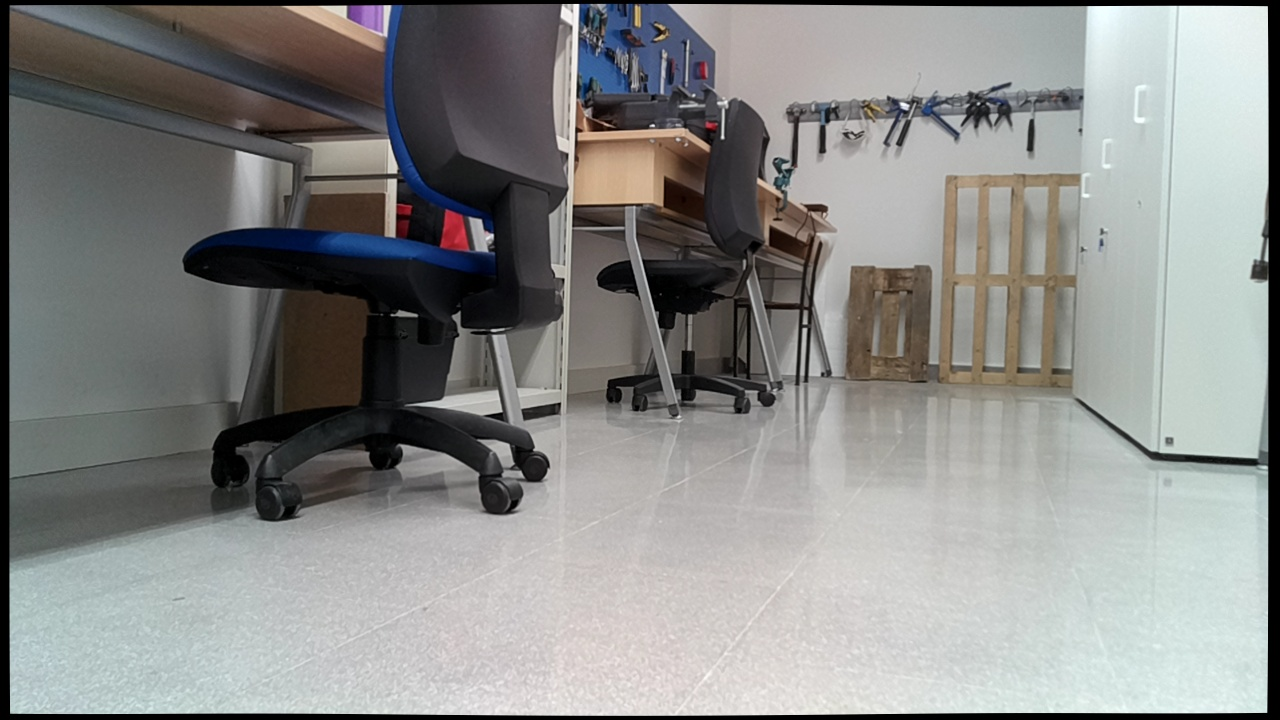
\includegraphics[height=6cm,width=\textwidth]{imgs/lr3.png}
    \caption{RGB}

  \end{subfigure}
\end{figure}

\begin{figure}[H]
  \centering
  \begin{subfigure}[b]{0.47\textwidth}
    \centering
    \includegraphics[height=6cm,width=\textwidth]{imgs/lc4.png}
    \caption{Point cloud}

  \end{subfigure}
  \hfill
  \begin{subfigure}[b]{0.47\textwidth}
    \centering
    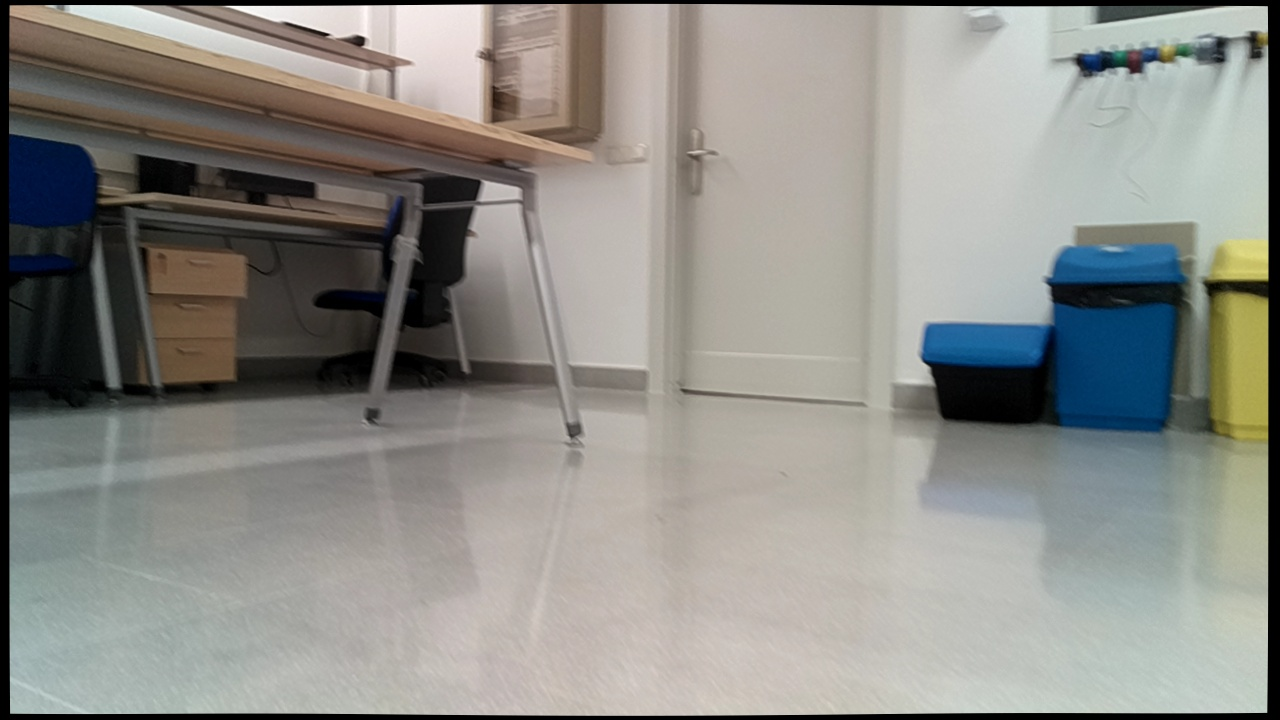
\includegraphics[height=6cm,width=\textwidth]{imgs/lr4.png}
    \caption{RGB}

  \end{subfigure}
\end{figure}

\begin{figure}[H]
  \centering
  \begin{subfigure}[b]{0.47\textwidth}
    \centering
    \includegraphics[height=6cm,width=\textwidth]{imgs/lc5.png}
    \caption{Point cloud}

  \end{subfigure}
  \hfill
  \begin{subfigure}[b]{0.47\textwidth}
    \centering
    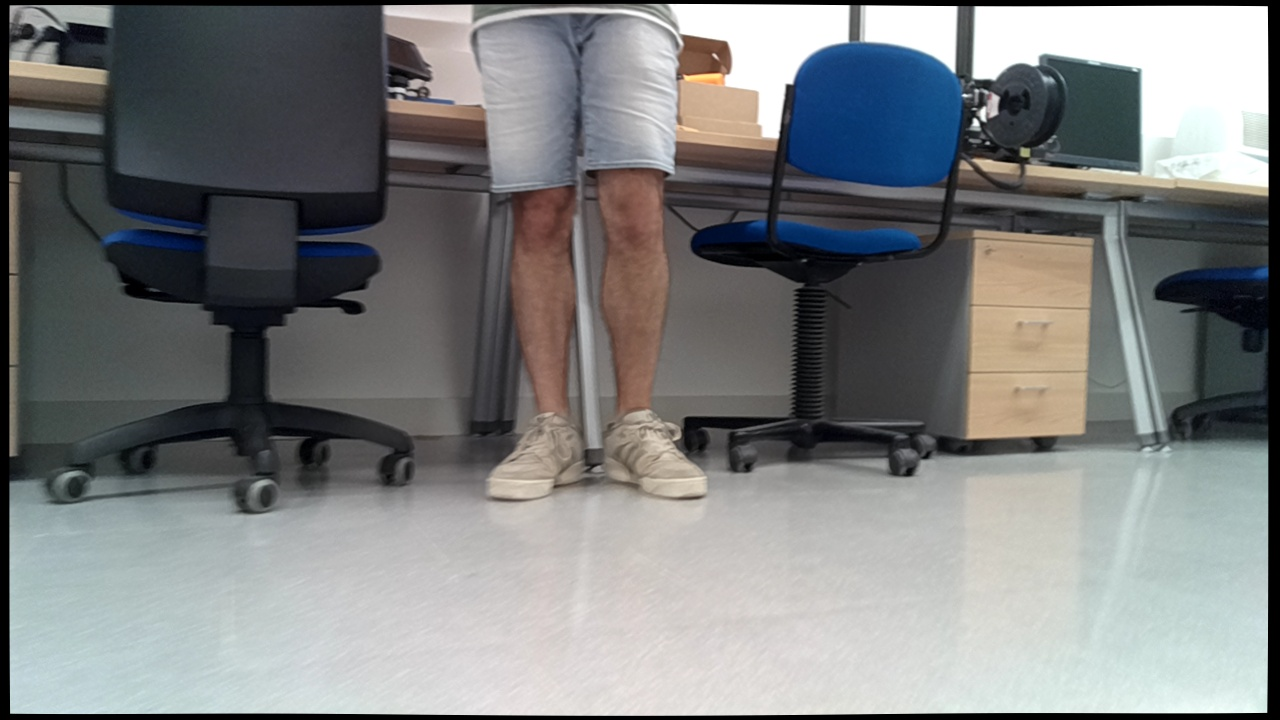
\includegraphics[height=6cm,width=\textwidth]{imgs/lr5.png}
    \caption{RGB}

  \end{subfigure}
\end{figure}

\begin{figure}[H]
  \centering
  \begin{subfigure}[b]{0.47\textwidth}
    \centering
    
\includegraphics[height=6cm,width=\textwidth]{imgs/cc (1).png}
    \caption{Point cloud}

  \end{subfigure}
  \hfill
  \begin{subfigure}[b]{0.47\textwidth}
    \centering
    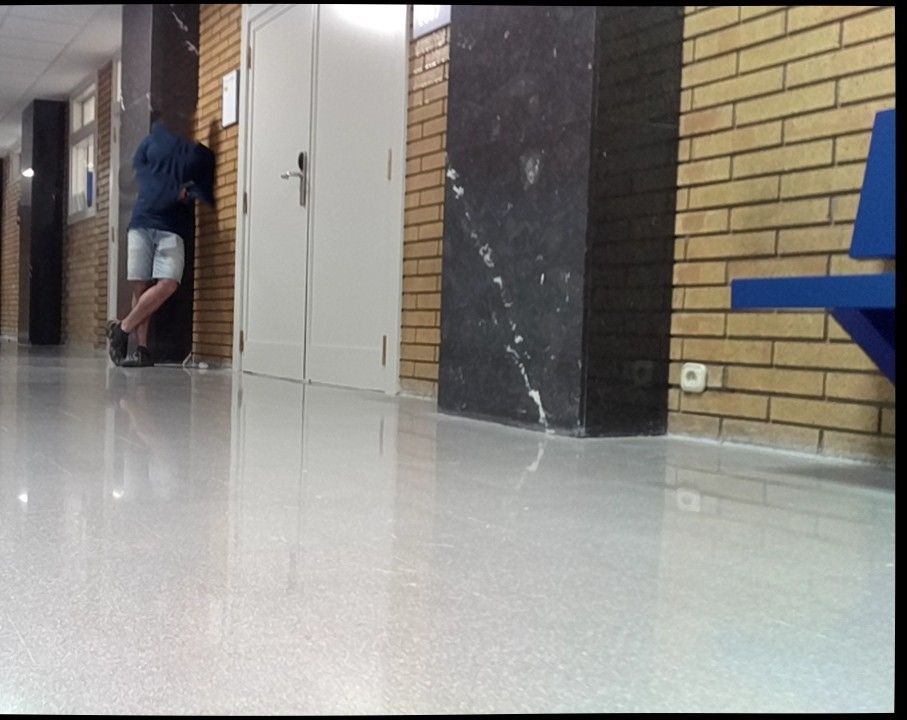
\includegraphics[height=6cm,width=\textwidth]{imgs/cr1.jpg}
    \caption{RGB}

  \end{subfigure}
\end{figure}

\begin{figure}[H]
  \centering
  \begin{subfigure}[b]{0.47\textwidth}
    \centering
    
\includegraphics[height=6cm,width=\textwidth]{imgs/cc (4).png}
    \caption{Point cloud}

  \end{subfigure}
  \hfill
  \begin{subfigure}[b]{0.47\textwidth}
    \centering
    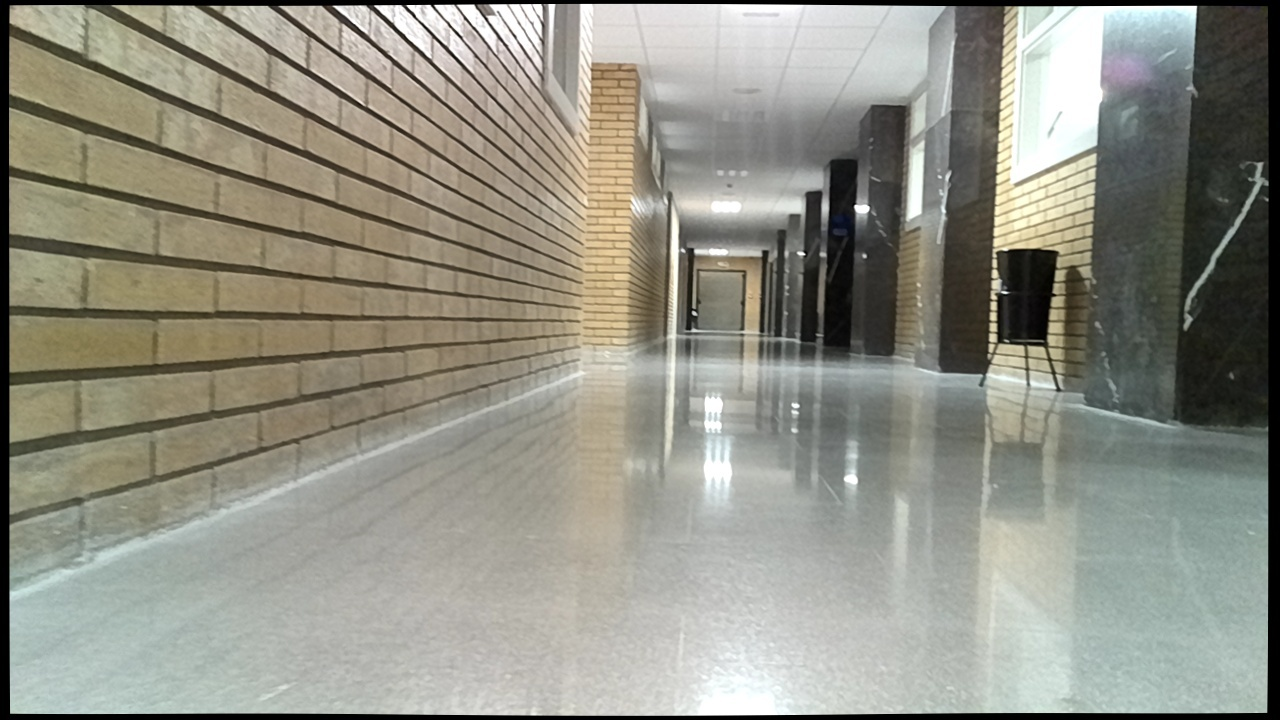
\includegraphics[height=6cm,width=\textwidth]{imgs/cr4.jpg}
    \caption{RGB}

  \end{subfigure}
\end{figure}

\begin{figure}[H]
  \centering
  \begin{subfigure}[b]{0.47\textwidth}
    \centering
    \includegraphics[height=6cm,width=\textwidth]{imgs/cc (3).png}
    \caption{Point cloud}

  \end{subfigure}
  \hfill
  \begin{subfigure}[b]{0.47\textwidth}
    \centering
    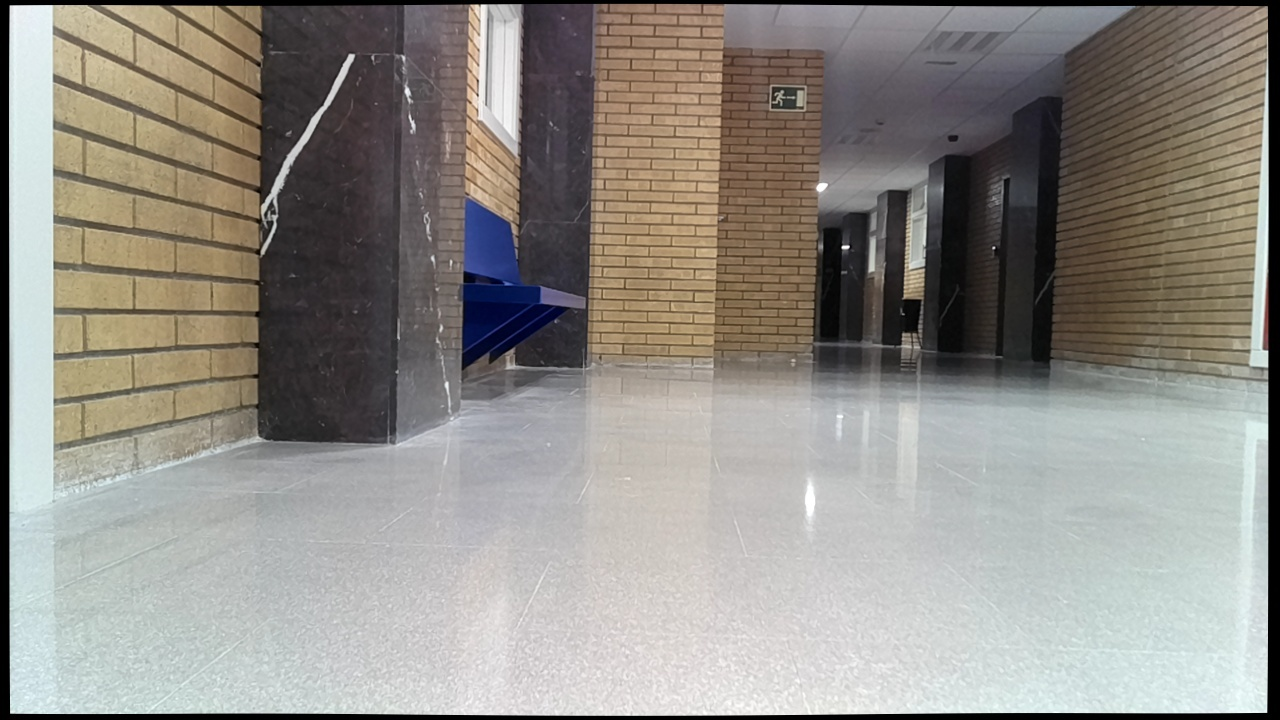
\includegraphics[height=6cm,width=\textwidth]{imgs/cr3.jpg}
    \caption{RGB}

  \end{subfigure}
\end{figure}

\end{document}
